\documentclass[10pt]{article} 
\usepackage{amsmath}
\usepackage{amssymb}
\usepackage{graphicx}
\usepackage{color}
\usepackage{soul} %% to use highlighting with \hl{} 
\usepackage{setspace}
\doublespacing 
% Text layout
\topmargin 0.0cm
\oddsidemargin 0.5cm
\evensidemargin 0.5cm
\textwidth 16cm 
\textheight 21cm
\usepackage[labelfont=bf,labelsep=period,justification=raggedright]{caption}
\usepackage{hyperref}
\date{}

\pagestyle{myheadings}
\usepackage{bm} % to get bold greek letters
\providecommand{\e}[1]{\ensuremath{\times 10^{#1}}}
\usepackage{caption}
\DeclareCaptionLabelFormat{continued}{#1~#2 (Continued)}
\captionsetup[ContinuedFloat]{labelformat=continued}

\begin{document}


% Supplemental figure 1 
% Results from all 89 DIAGRAM Loci 
\begin{figure}
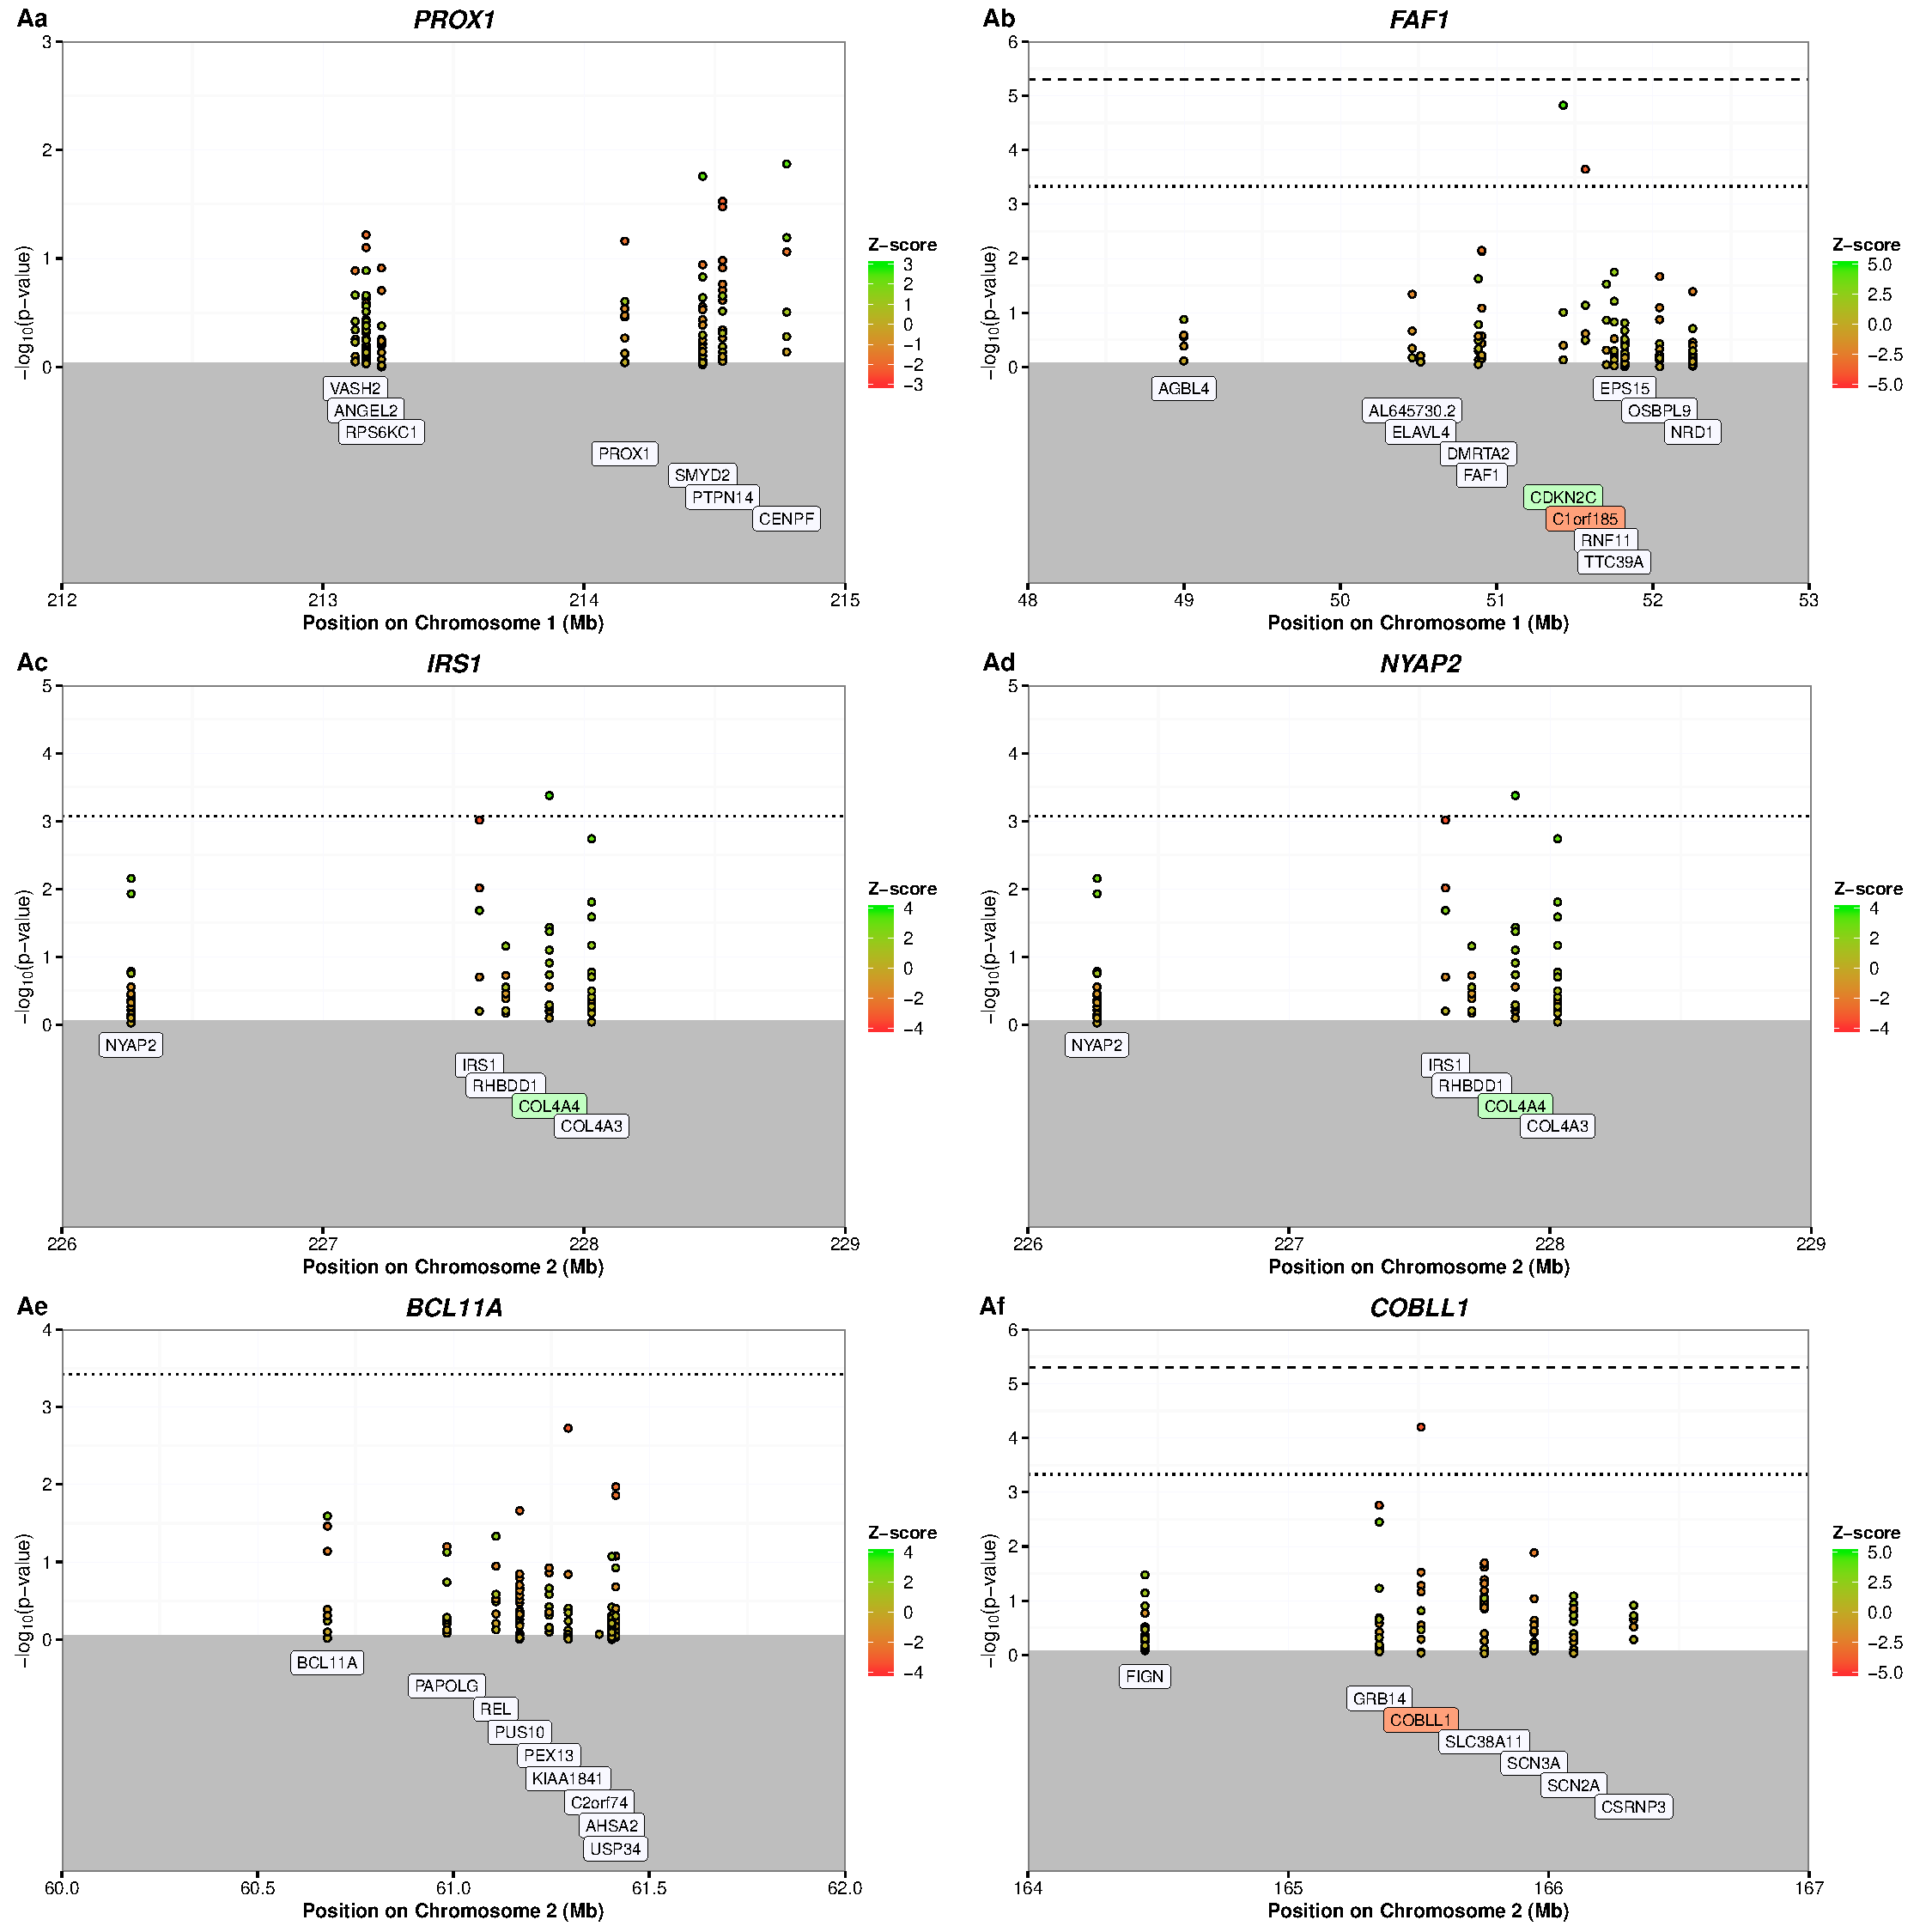
\includegraphics[width=\textwidth]{sup_fig1_part1_locusArray.pdf}
	\caption{\textbf{MetaXcan profiles at T2D-associated loci} We tested for association between predicted gene expression and T2D at $\sim2$ Mb genomic regions encompassing putative T2D genes implicated by the top $1,000$ SNPs associated with T2D from the DIAGRAM trans-ethnic meta-analysis of GWASs using $42$ tissue-level prediction models. The gene about which the genomic region is centered is indicated at the top of each panel. The solid, dashed, and dotted line denote significance correcting for the total number of tests performed across all models, genome-wide significance in a single model ($10,000$ tests), and locus-wide significance, respectively. Genomic position (Mb) and significance ($-\log_{10}$(p-value)) for each predicted gene expression value (from a particular tissue model) are shown on the $x$ and $y$-axis, respectively. Gene labels are shown in the gray region and are positioned at the transcription start site (TSS). Moreover, the color of each point corresponds to the magnitude and sign of the $Z$-score where positive and negative $Z$-scores are colored green and red, respectively.} 
    \label{fig:supp.locus_array_fig1_part1}
\end{figure}

\begin{figure}
\ContinuedFloat
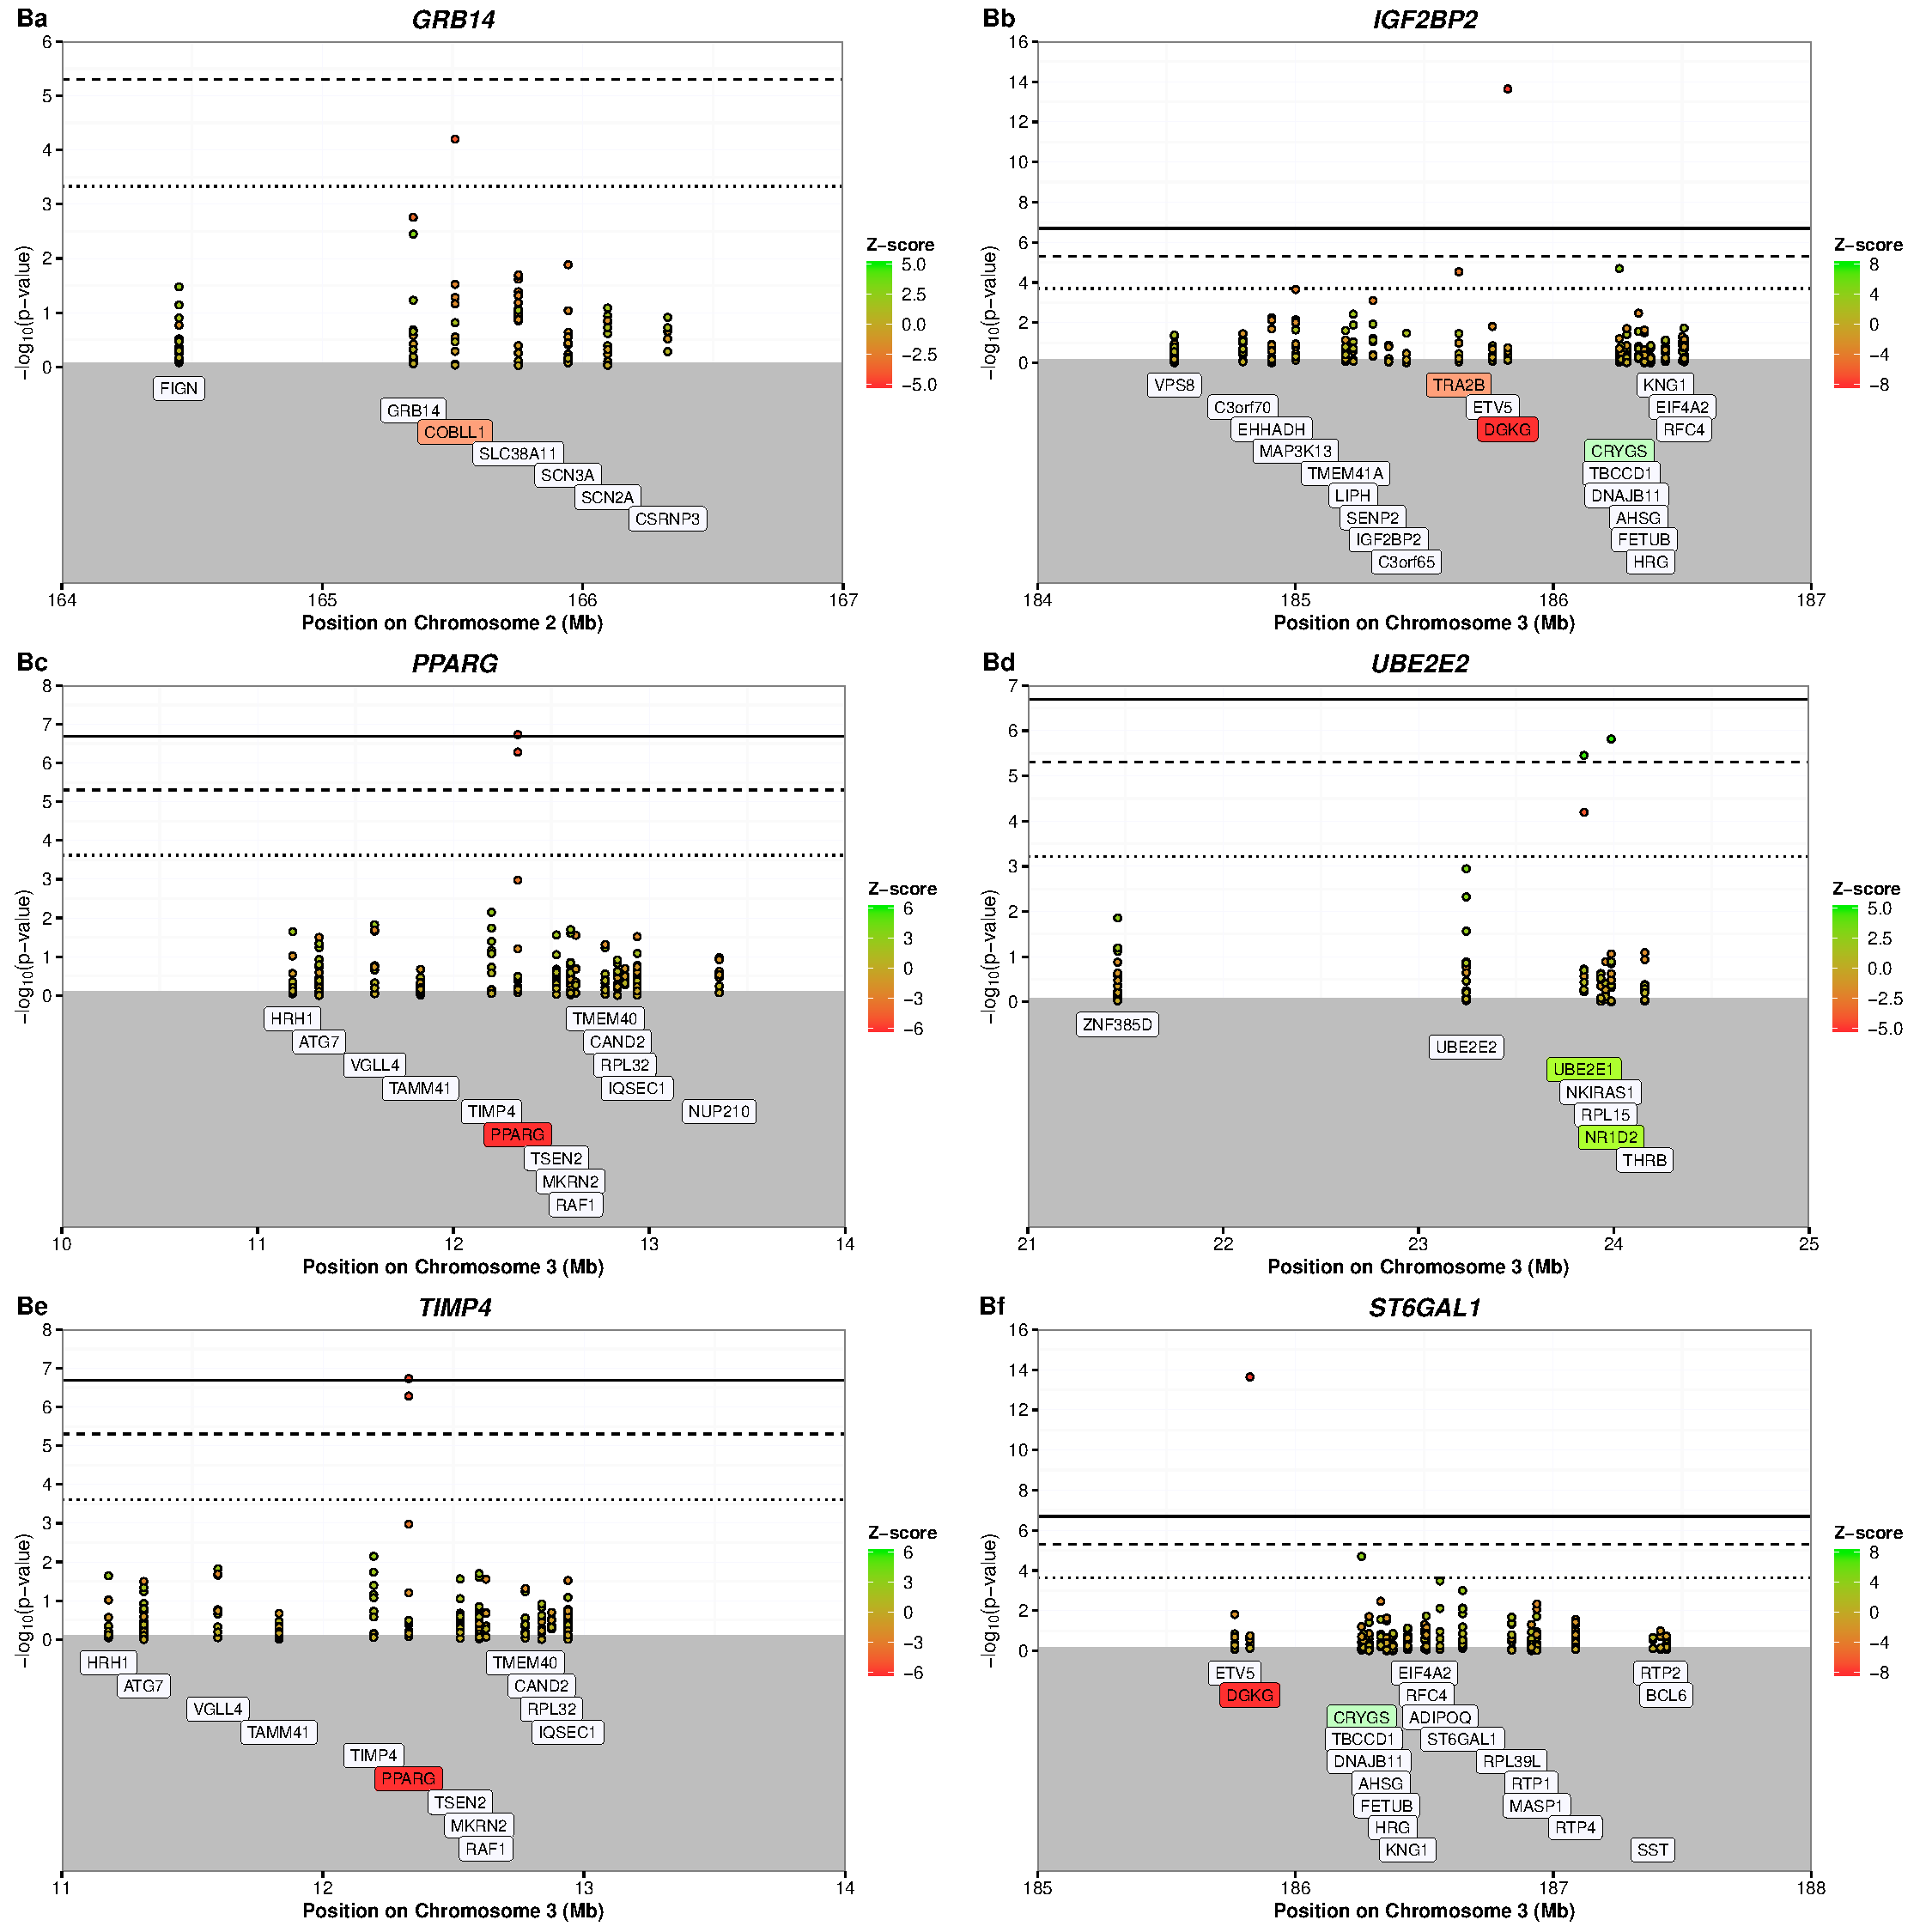
\includegraphics[width=\textwidth]{sup_fig1_part2_locusArray.pdf}
	\caption{\textbf{MetaXcan profiles at T2D-associated loci} We tested for association between predicted gene expression and T2D at $\sim2$ Mb genomic regions encompassing putative T2D genes implicated by the top $1,000$ SNPs associated with T2D from the DIAGRAM trans-ethnic meta-analysis of GWASs using $42$ tissue-level prediction models. The gene about which the genomic region is centered is indicated at the top of each panel. The solid, dashed, and dotted line denote significance correcting for the total number of tests performed across all models, genome-wide significance in a single model ($10,000$ tests), and locus-wide significance, respectively. Genomic position (Mb) and significance ($-\log_{10}$(p-value)) for each predicted gene expression value (from a particular tissue model) are shown on the $x$ and $y$-axis, respectively. Gene labels are shown in the gray region and are positioned at the transcription start site (TSS). Moreover, color corresponds to the magnitude and sign of the $Z$-score where positive and negative $Z$-scores are colored green and red, respectively.} 
    \label{fig:supp.locus_array_fig1_part2}
\end{figure}

\begin{figure}
\ContinuedFloat
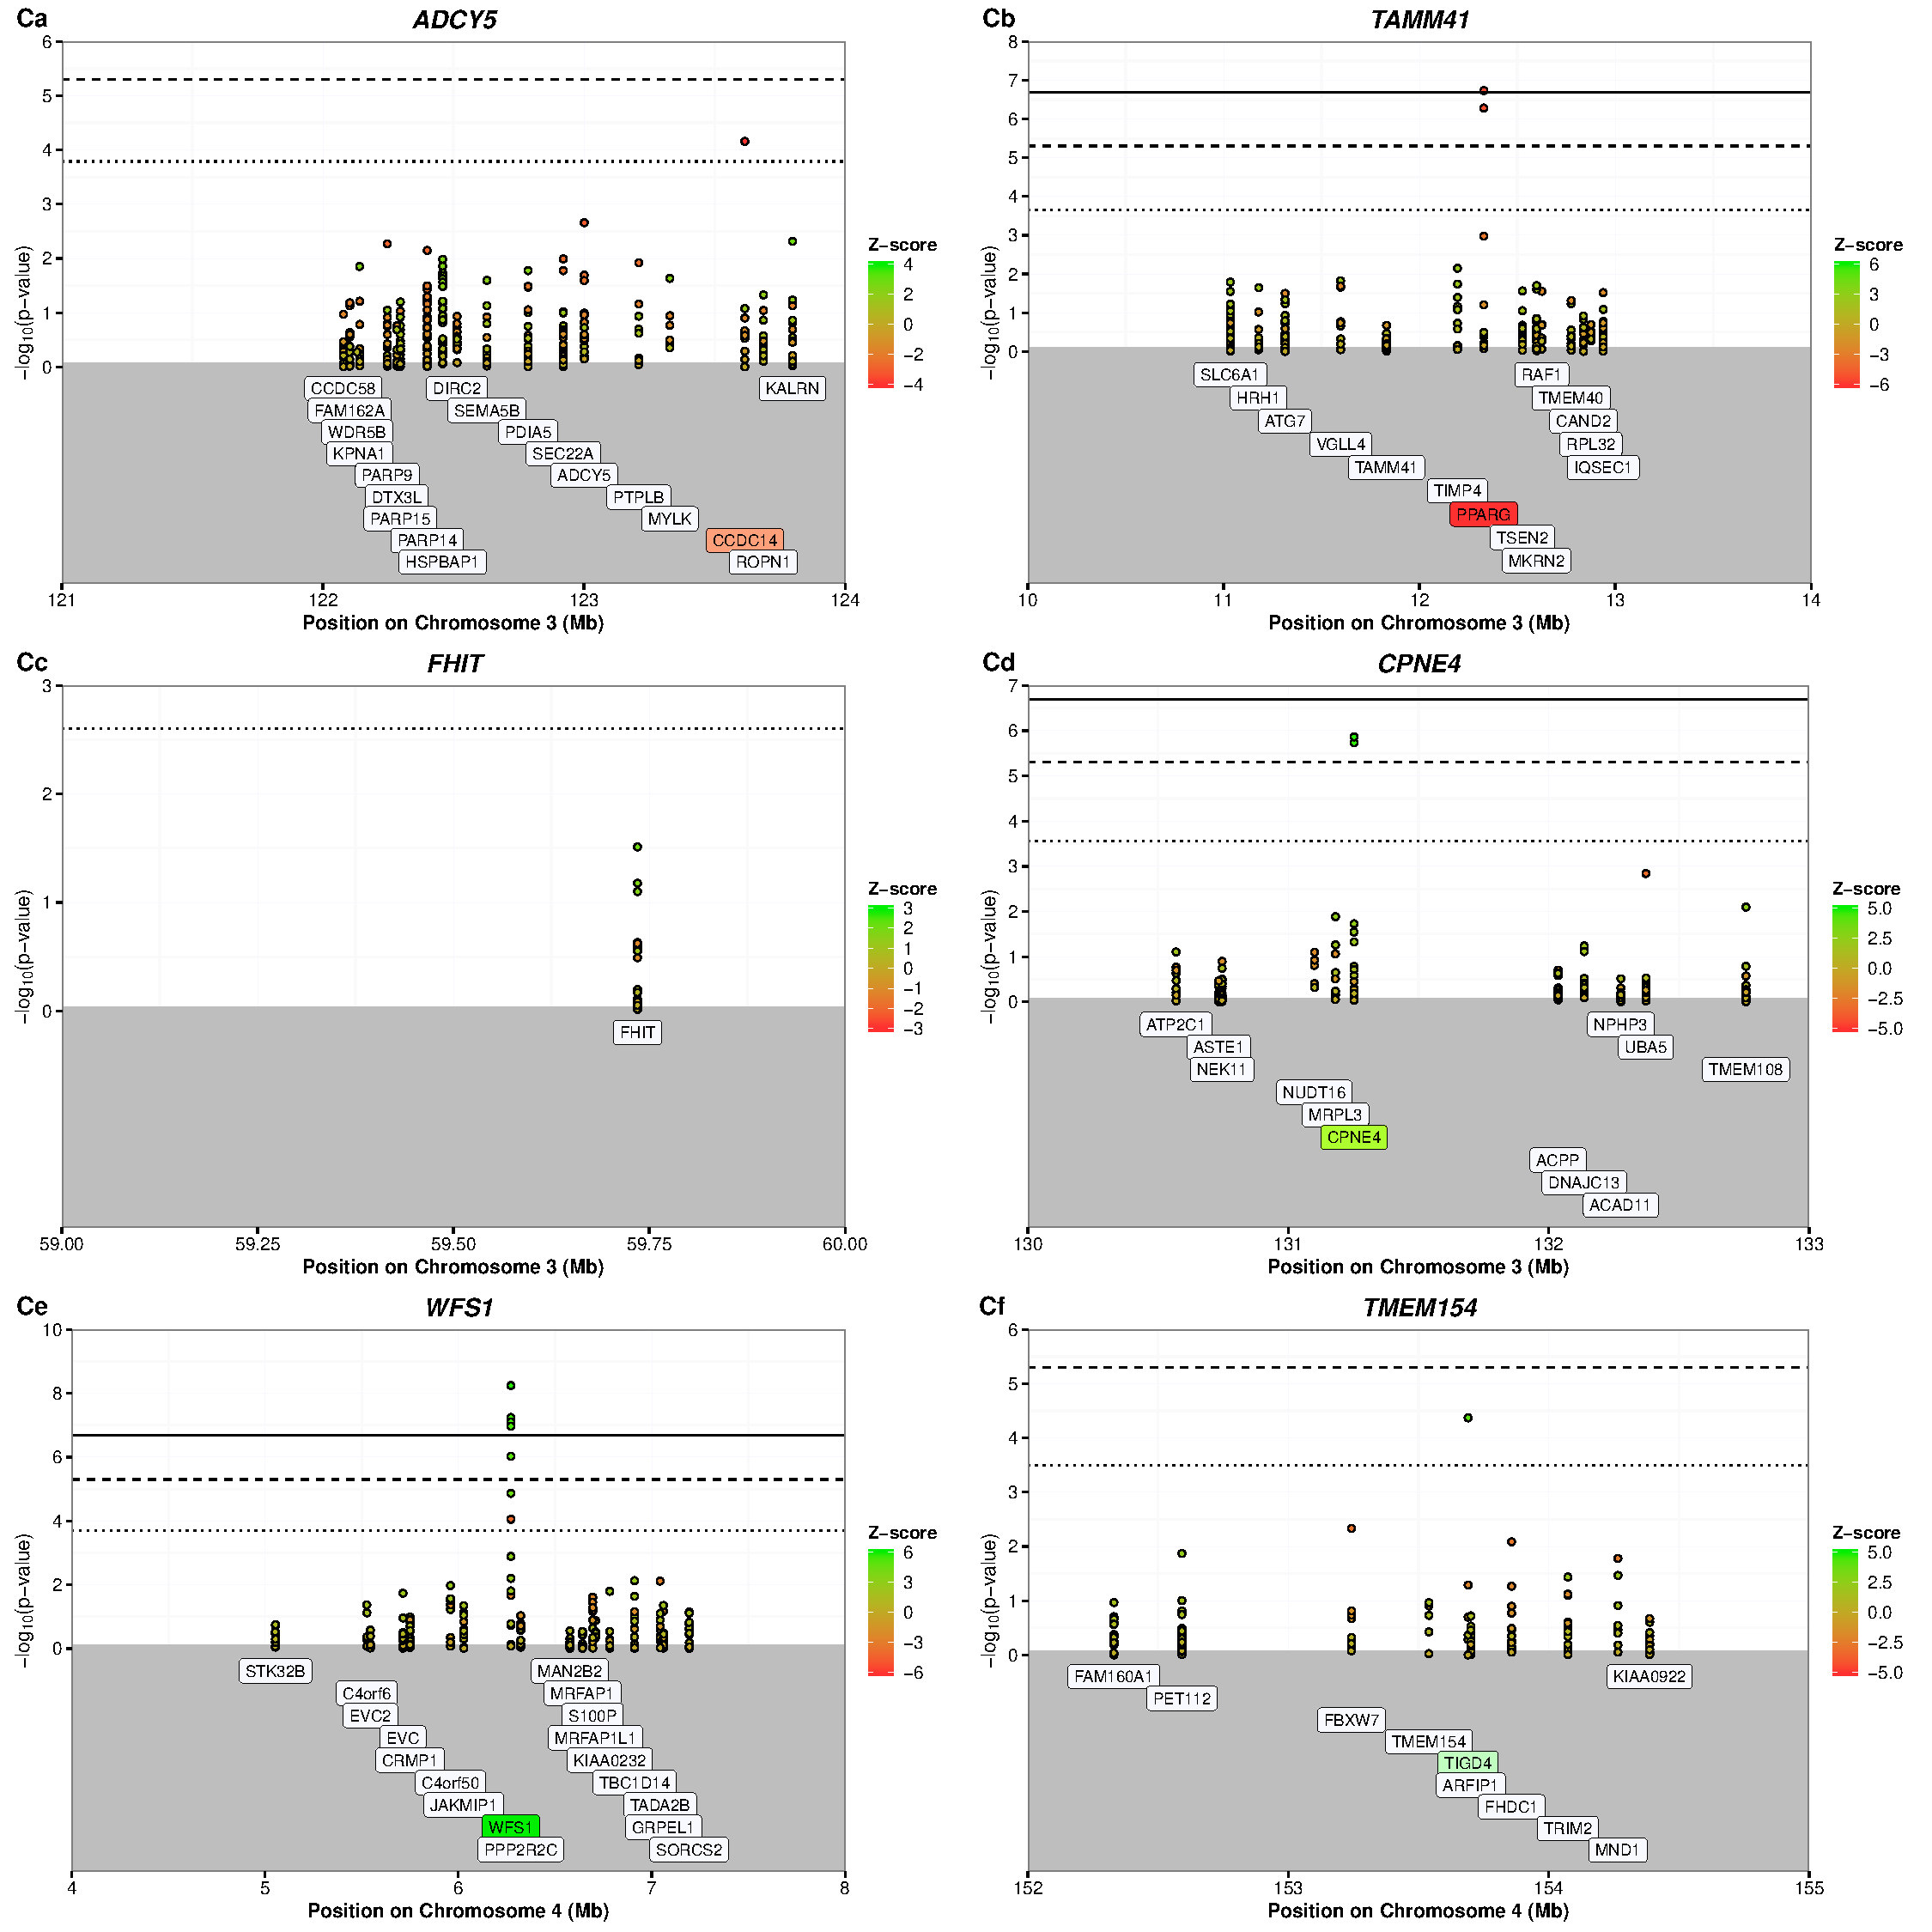
\includegraphics[width=\textwidth]{sup_fig1_part3_locusArray.pdf}
	\caption{\textbf{MetaXcan profiles at T2D-associated loci} We tested for association between predicted gene expression and T2D at $\sim2$ Mb genomic regions encompassing putative T2D genes implicated by the top $1,000$ SNPs associated with T2D from the DIAGRAM trans-ethnic meta-analysis of GWASs using $42$ tissue-level prediction models. The gene about which the genomic region is centered is indicated at the top of each panel. The solid, dashed, and dotted line denote significance correcting for the total number of tests performed across all models, genome-wide significance in a single model ($10,000$ tests), and locus-wide significance, respectively. Genomic position (Mb) and significance ($-\log_{10}$(p-value)) for each predicted gene expression value (from a particular tissue model) are shown on the $x$ and $y$-axis, respectively. Gene labels are shown in the gray region and are positioned at the transcription start site (TSS). Moreover, color corresponds to the magnitude and sign of the $Z$-score where positive and negative $Z$-scores are colored green and red, respectively.} 
    \label{fig:supp.locus_array_fig1_part3}
\end{figure}

\begin{figure}
\ContinuedFloat
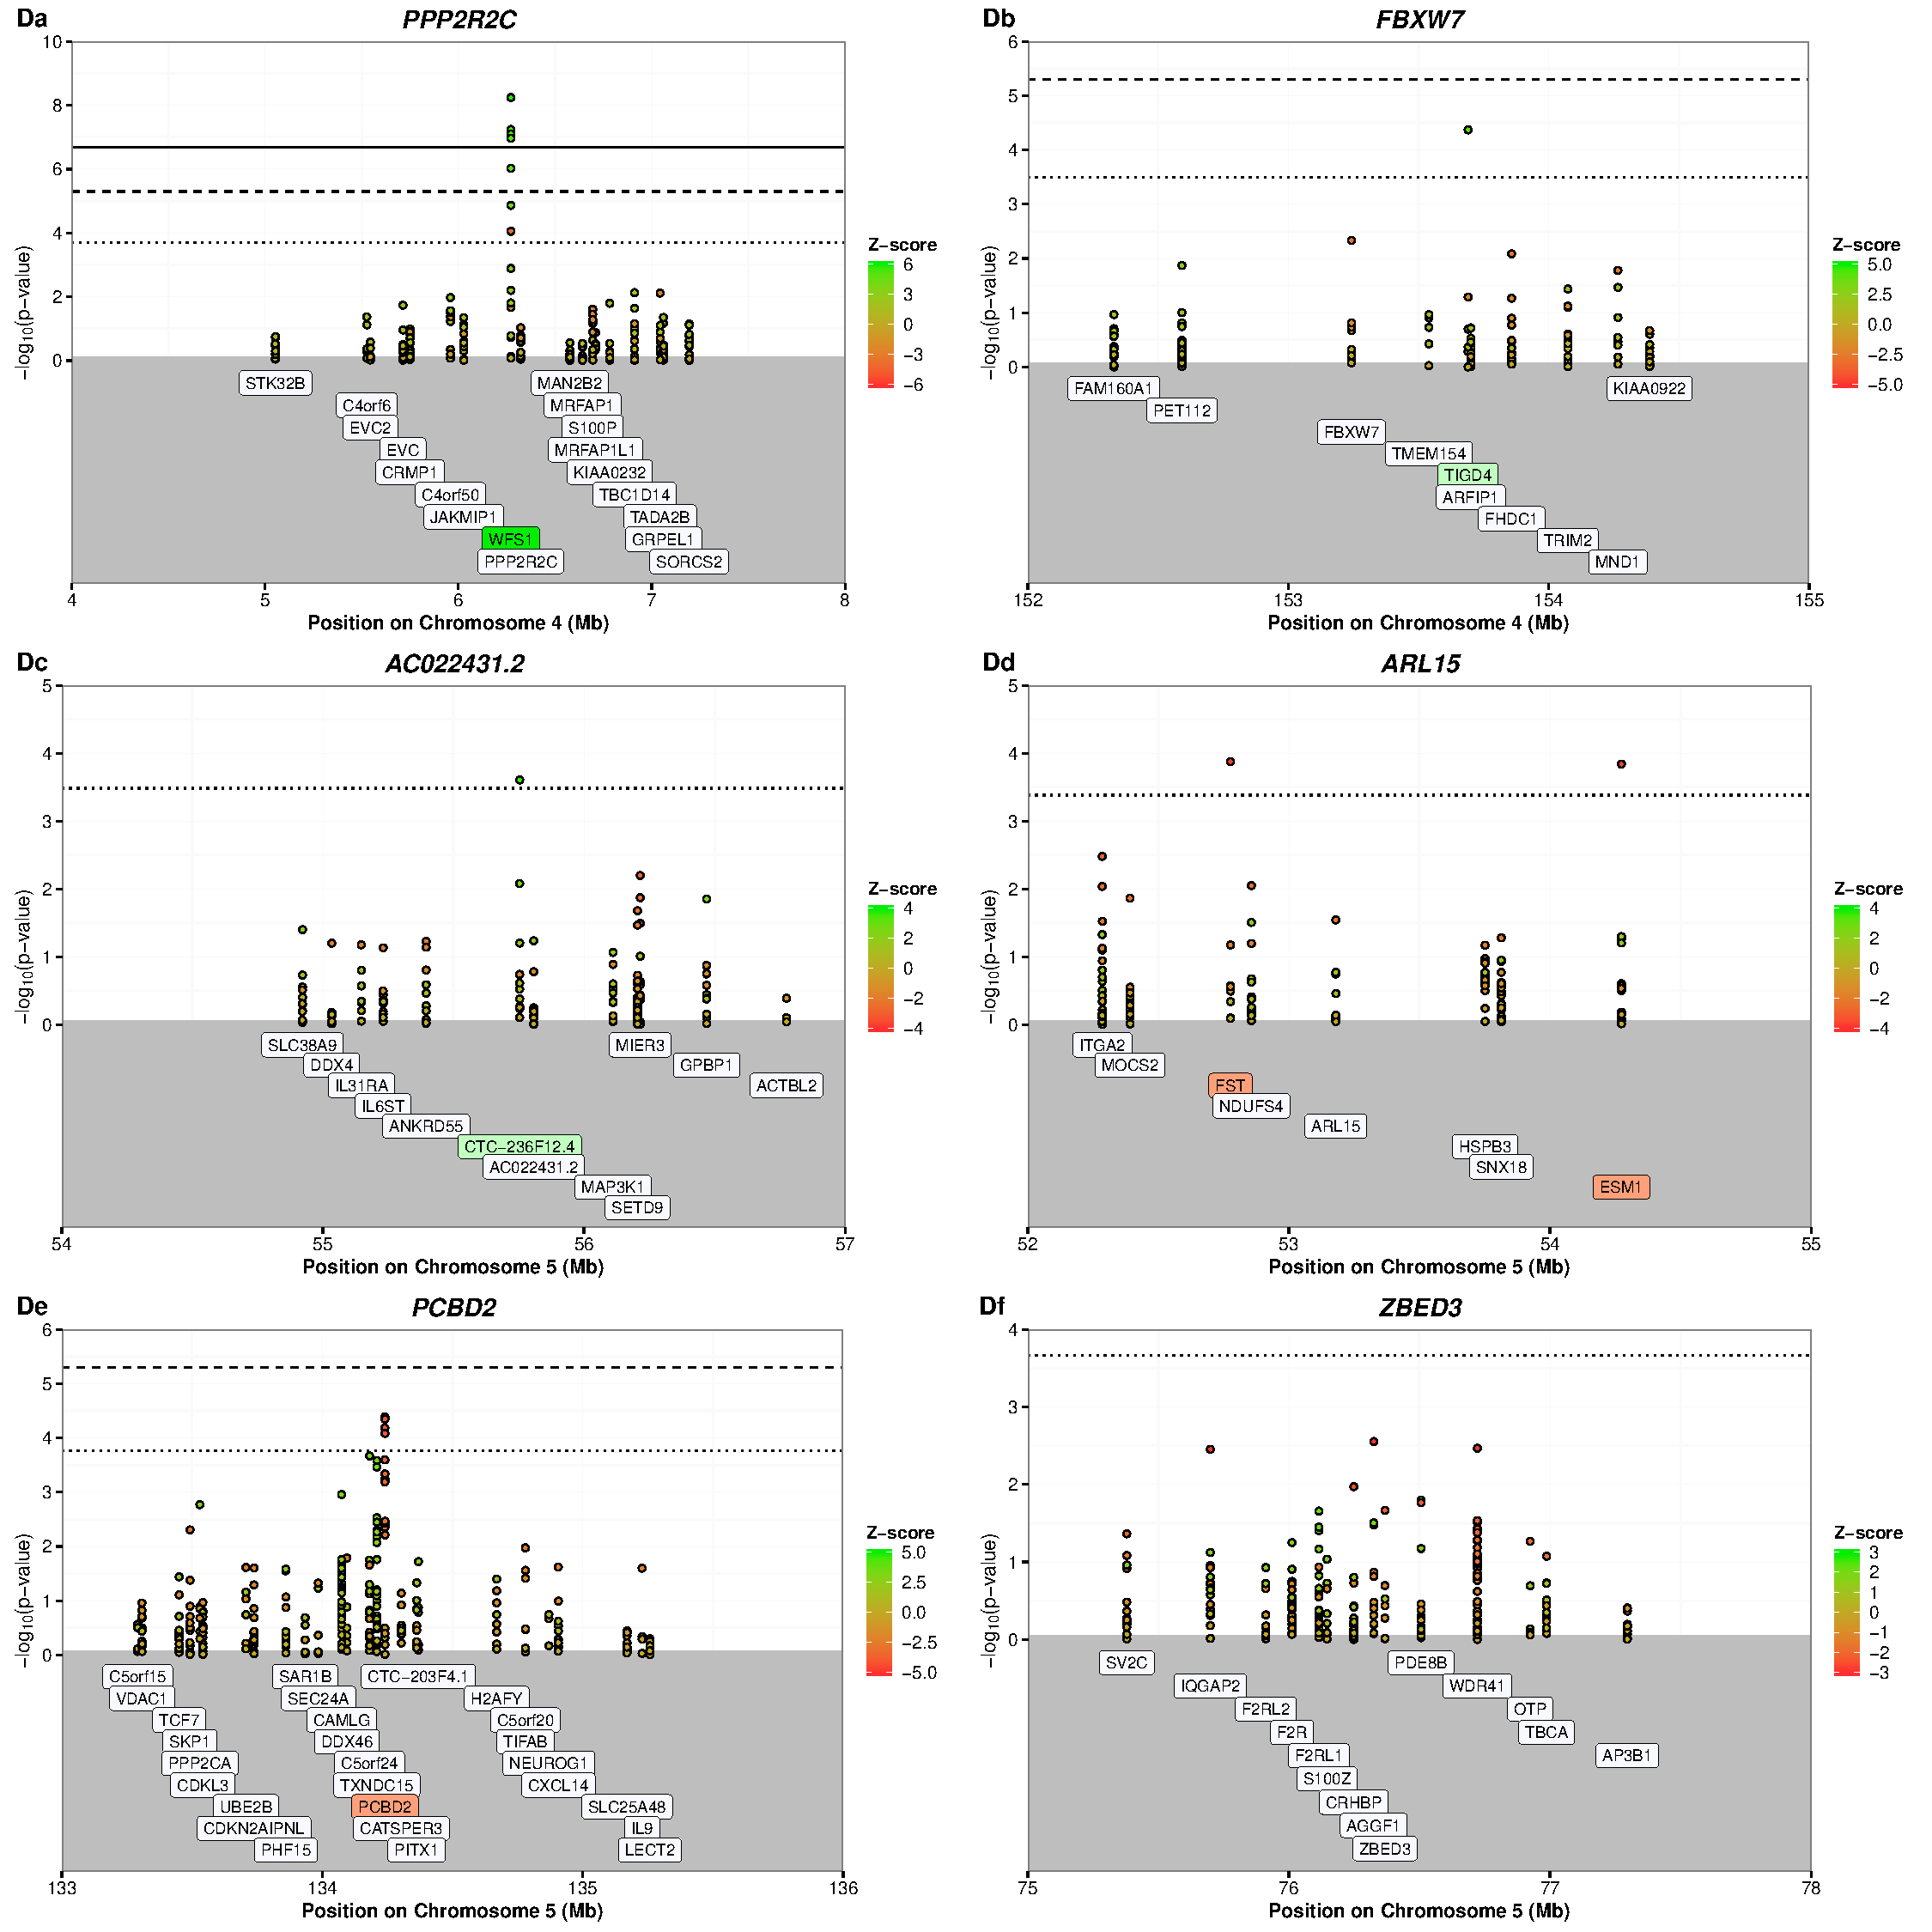
\includegraphics[width=\textwidth]{sup_fig1_part4_locusArray.pdf}
	\caption{\textbf{MetaXcan profiles at T2D-associated loci} We tested for association between predicted gene expression and T2D at $\sim2$ Mb genomic regions encompassing putative T2D genes implicated by the top $1,000$ SNPs associated with T2D from the DIAGRAM trans-ethnic meta-analysis of GWASs using $42$ tissue-level prediction models. The gene about which the genomic region is centered is indicated at the top of each panel. The solid, dashed, and dotted line denote significance correcting for the total number of tests performed across all models, genome-wide significance in a single model ($10,000$ tests), and locus-wide significance, respectively. Genomic position (Mb) and significance ($-\log_{10}$(p-value)) for each predicted gene expression value (from a particular tissue model) are shown on the $x$ and $y$-axis, respectively. Gene labels are shown in the gray region and are positioned at the transcription start site (TSS). Moreover, color corresponds to the magnitude and sign of the $Z$-score where positive and negative $Z$-scores are colored green and red, respectively.} 
    \label{fig:supp.locus_array_fig1_part4}
\end{figure}

\begin{figure}
\ContinuedFloat
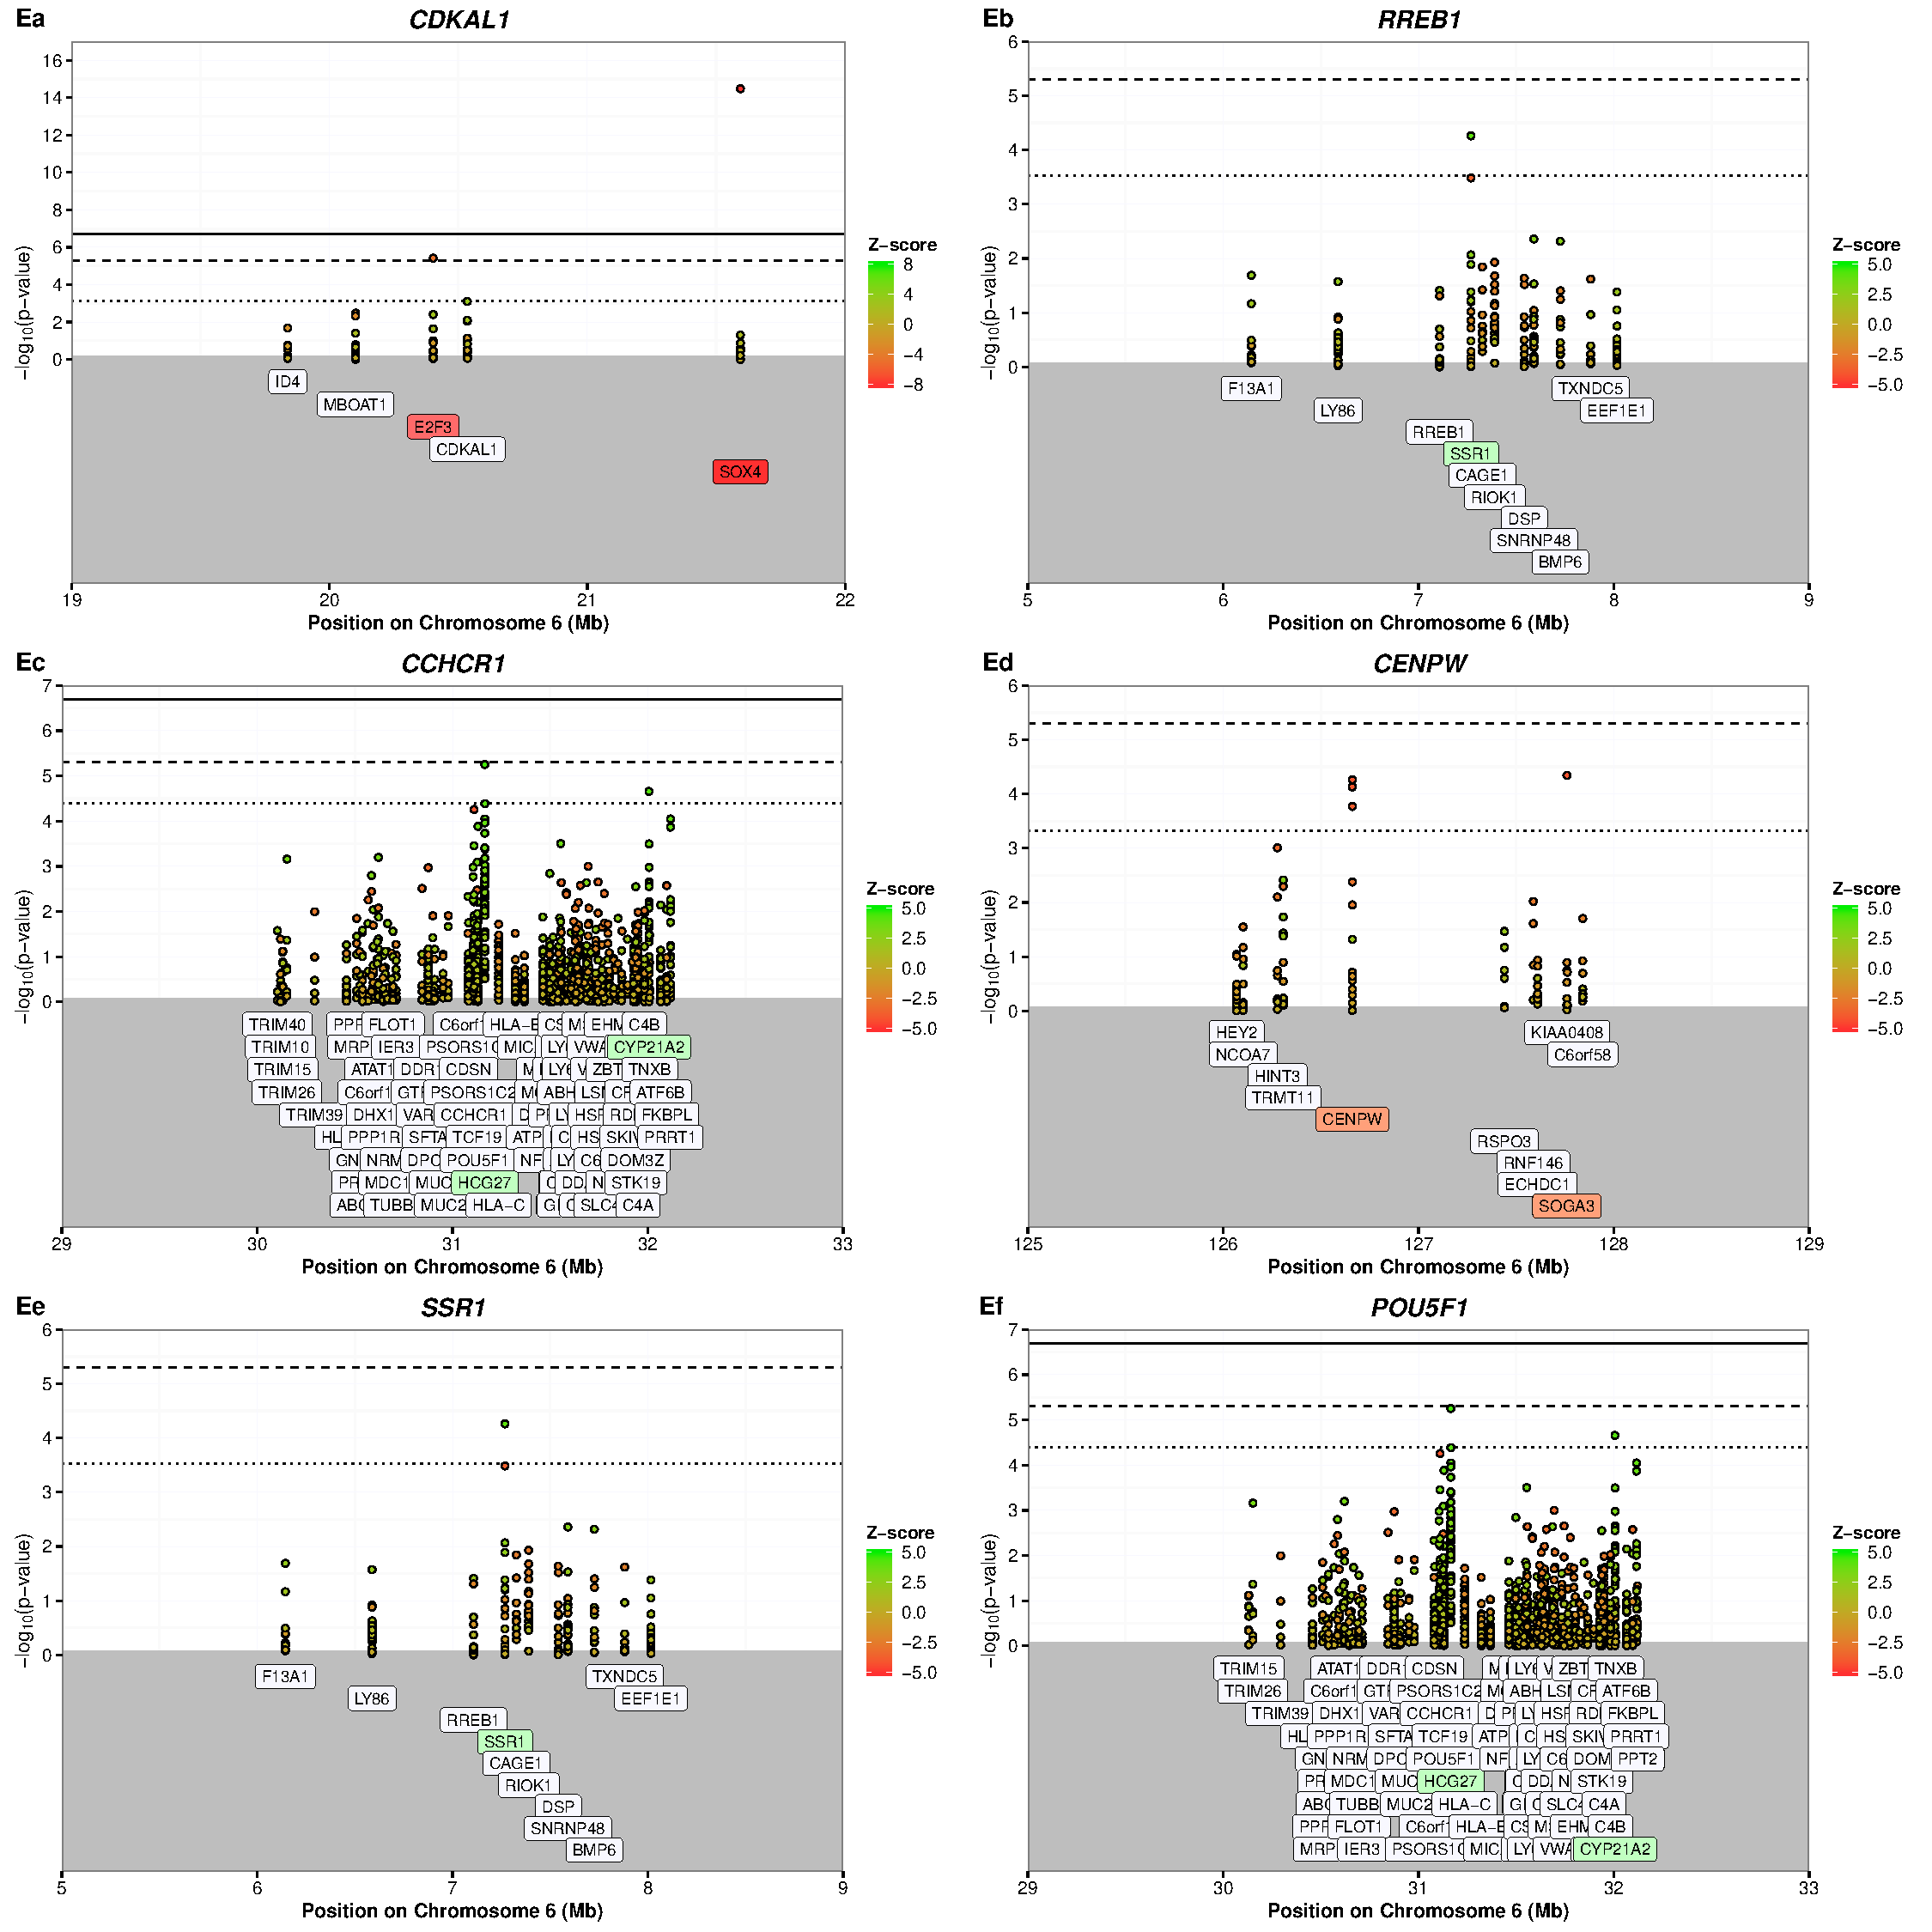
\includegraphics[width=\textwidth]{sup_fig1_part5_locusArray.pdf}
	\caption{\textbf{MetaXcan profiles at T2D-associated loci} We tested for association between predicted gene expression and T2D at $\sim2$ Mb genomic regions encompassing putative T2D genes implicated by the top $1,000$ SNPs associated with T2D from the DIAGRAM trans-ethnic meta-analysis of GWASs using $42$ tissue-level prediction models. The gene about which the genomic region is centered is indicated at the top of each panel. The solid, dashed, and dotted line denote significance correcting for the total number of tests performed across all models, genome-wide significance in a single model ($10,000$ tests), and locus-wide significance, respectively. Genomic position (Mb) and significance ($-\log_{10}$(p-value)) for each predicted gene expression value (from a particular tissue model) are shown on the $x$ and $y$-axis, respectively. Gene labels are shown in the gray region and are positioned at the transcription start site (TSS). Moreover, color corresponds to the magnitude and sign of the $Z$-score where positive and negative $Z$-scores are colored green and red, respectively.} 
    \label{fig:supp.locus_array_fig1_part5}
\end{figure}

\begin{figure}
\ContinuedFloat
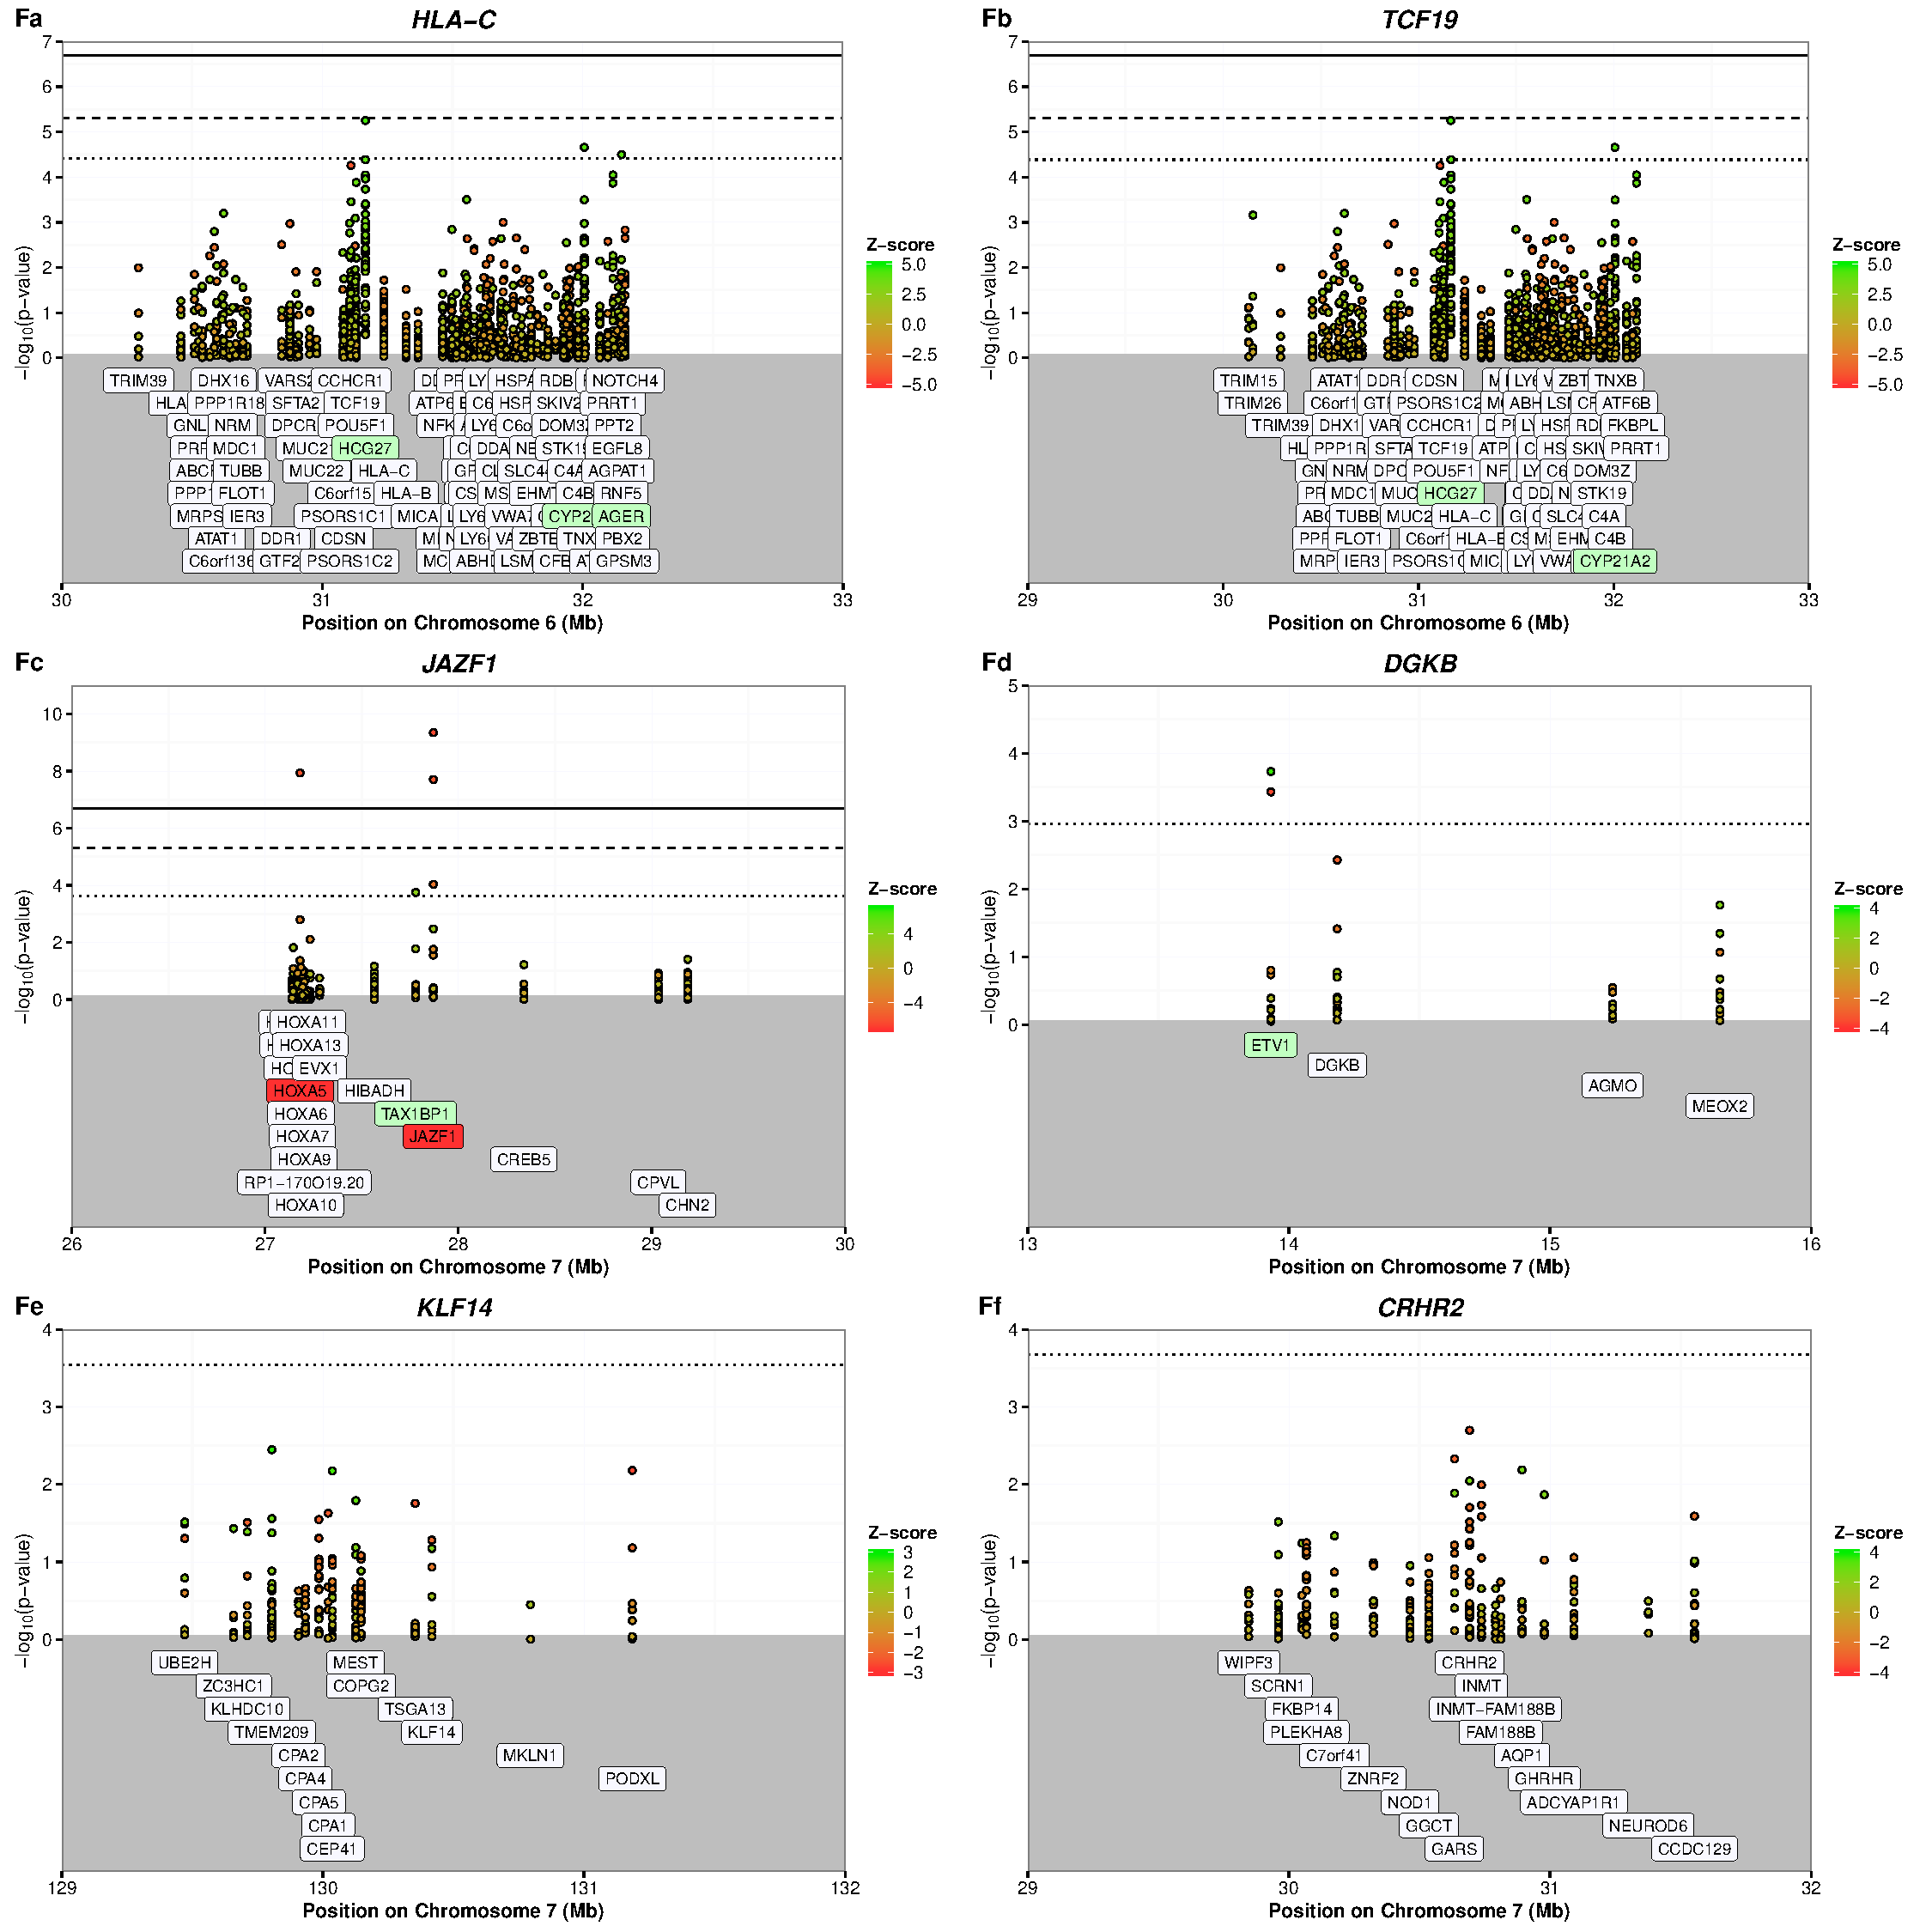
\includegraphics[width=\textwidth]{sup_fig1_part6_locusArray.pdf}
	\caption{\textbf{MetaXcan profiles at T2D-associated loci} We tested for association between predicted gene expression and T2D at $\sim2$ Mb genomic regions encompassing putative T2D genes implicated by the top $1,000$ SNPs associated with T2D from the DIAGRAM trans-ethnic meta-analysis of GWASs using $42$ tissue-level prediction models. The gene about which the genomic region is centered is indicated at the top of each panel. The solid, dashed, and dotted line denote significance correcting for the total number of tests performed across all models, genome-wide significance in a single model ($10,000$ tests), and locus-wide significance, respectively. Genomic position (Mb) and significance ($-\log_{10}$(p-value)) for each predicted gene expression value (from a particular tissue model) are shown on the $x$ and $y$-axis, respectively. Gene labels are shown in the gray region and are positioned at the transcription start site (TSS). Moreover, color corresponds to the magnitude and sign of the $Z$-score where positive and negative $Z$-scores are colored green and red, respectively.} 
    \label{fig:supp.locus_array_fig1_part6}
\end{figure}

\begin{figure}
\ContinuedFloat
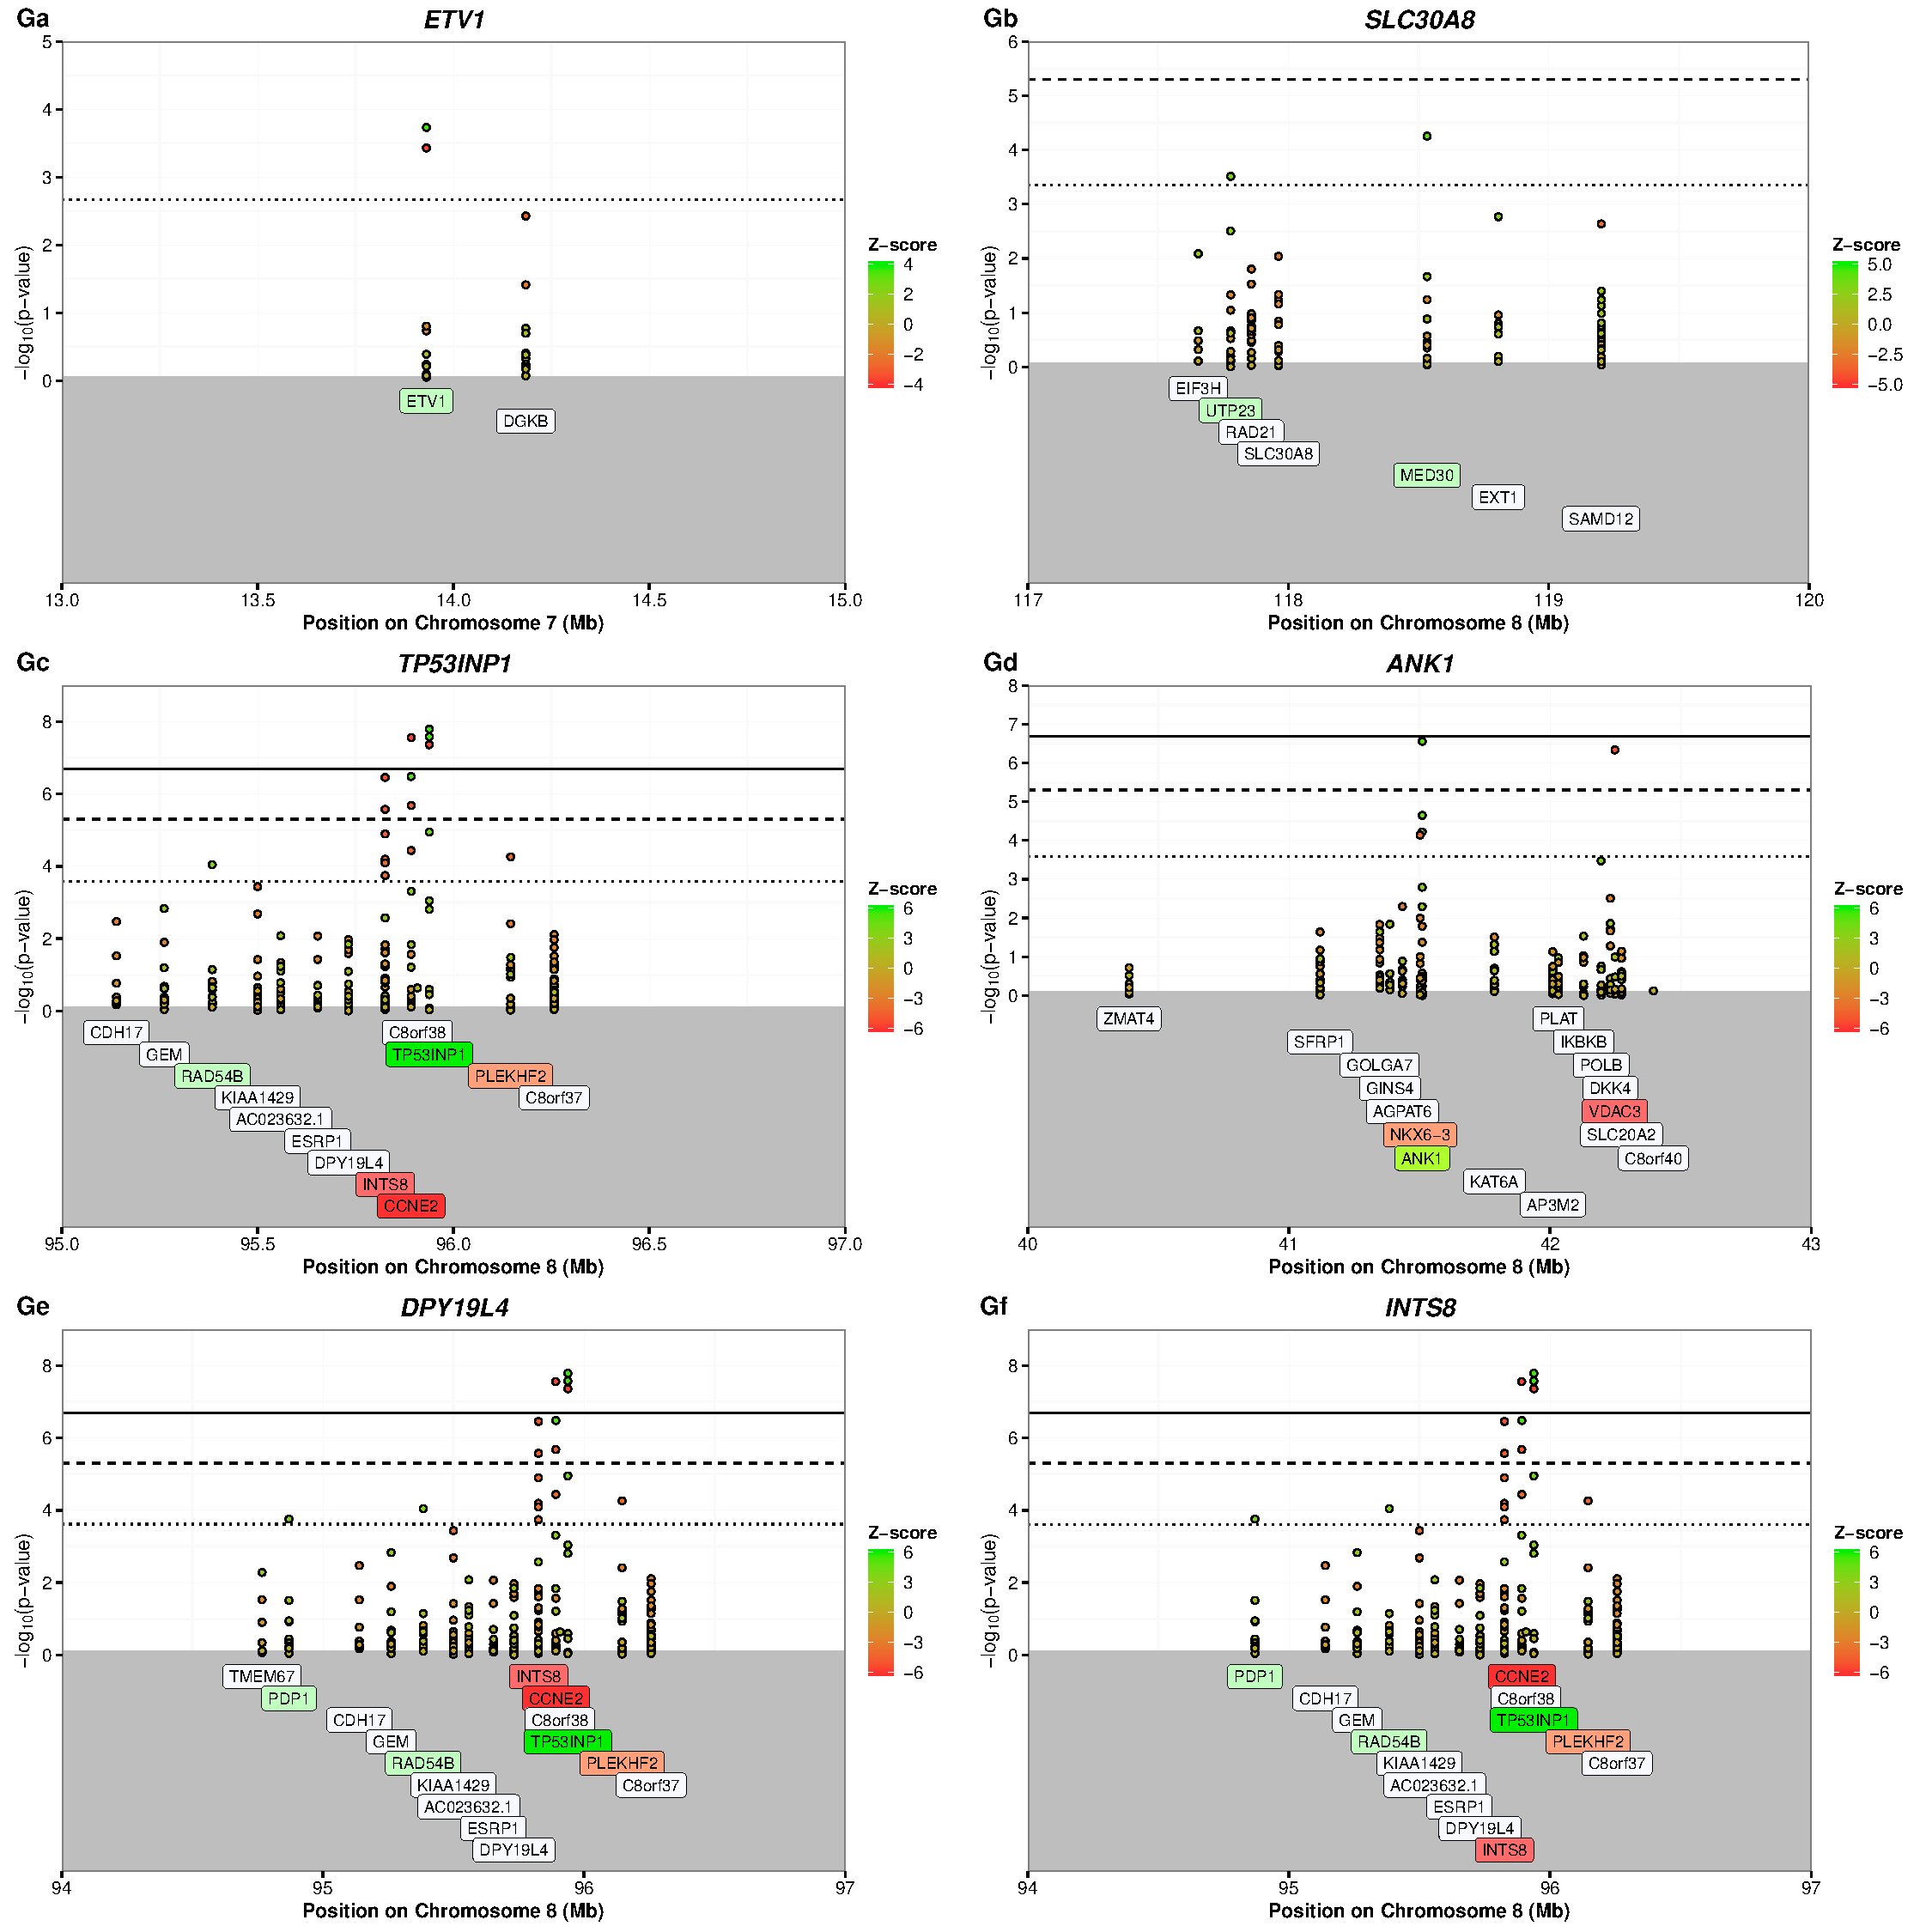
\includegraphics[width=\textwidth]{sup_fig1_part7_locusArray.pdf}
	\caption{\textbf{MetaXcan profiles at T2D-associated loci} We tested for association between predicted gene expression and T2D at $\sim2$ Mb genomic regions encompassing putative T2D genes implicated by the top $1,000$ SNPs associated with T2D from the DIAGRAM trans-ethnic meta-analysis of GWASs using $42$ tissue-level prediction models. The gene about which the genomic region is centered is indicated at the top of each panel. The solid, dashed, and dotted line denote significance correcting for the total number of tests performed across all models, genome-wide significance in a single model ($10,000$ tests), and locus-wide significance, respectively. Genomic position (Mb) and significance ($-\log_{10}$(p-value)) for each predicted gene expression value (from a particular tissue model) are shown on the $x$ and $y$-axis, respectively. Gene labels are shown in the gray region and are positioned at the transcription start site (TSS). Moreover, color corresponds to the magnitude and sign of the $Z$-score where positive and negative $Z$-scores are colored green and red, respectively.} 
    \label{fig:supp.locus_array_fig1_part7}
\end{figure}

\begin{figure}
\ContinuedFloat
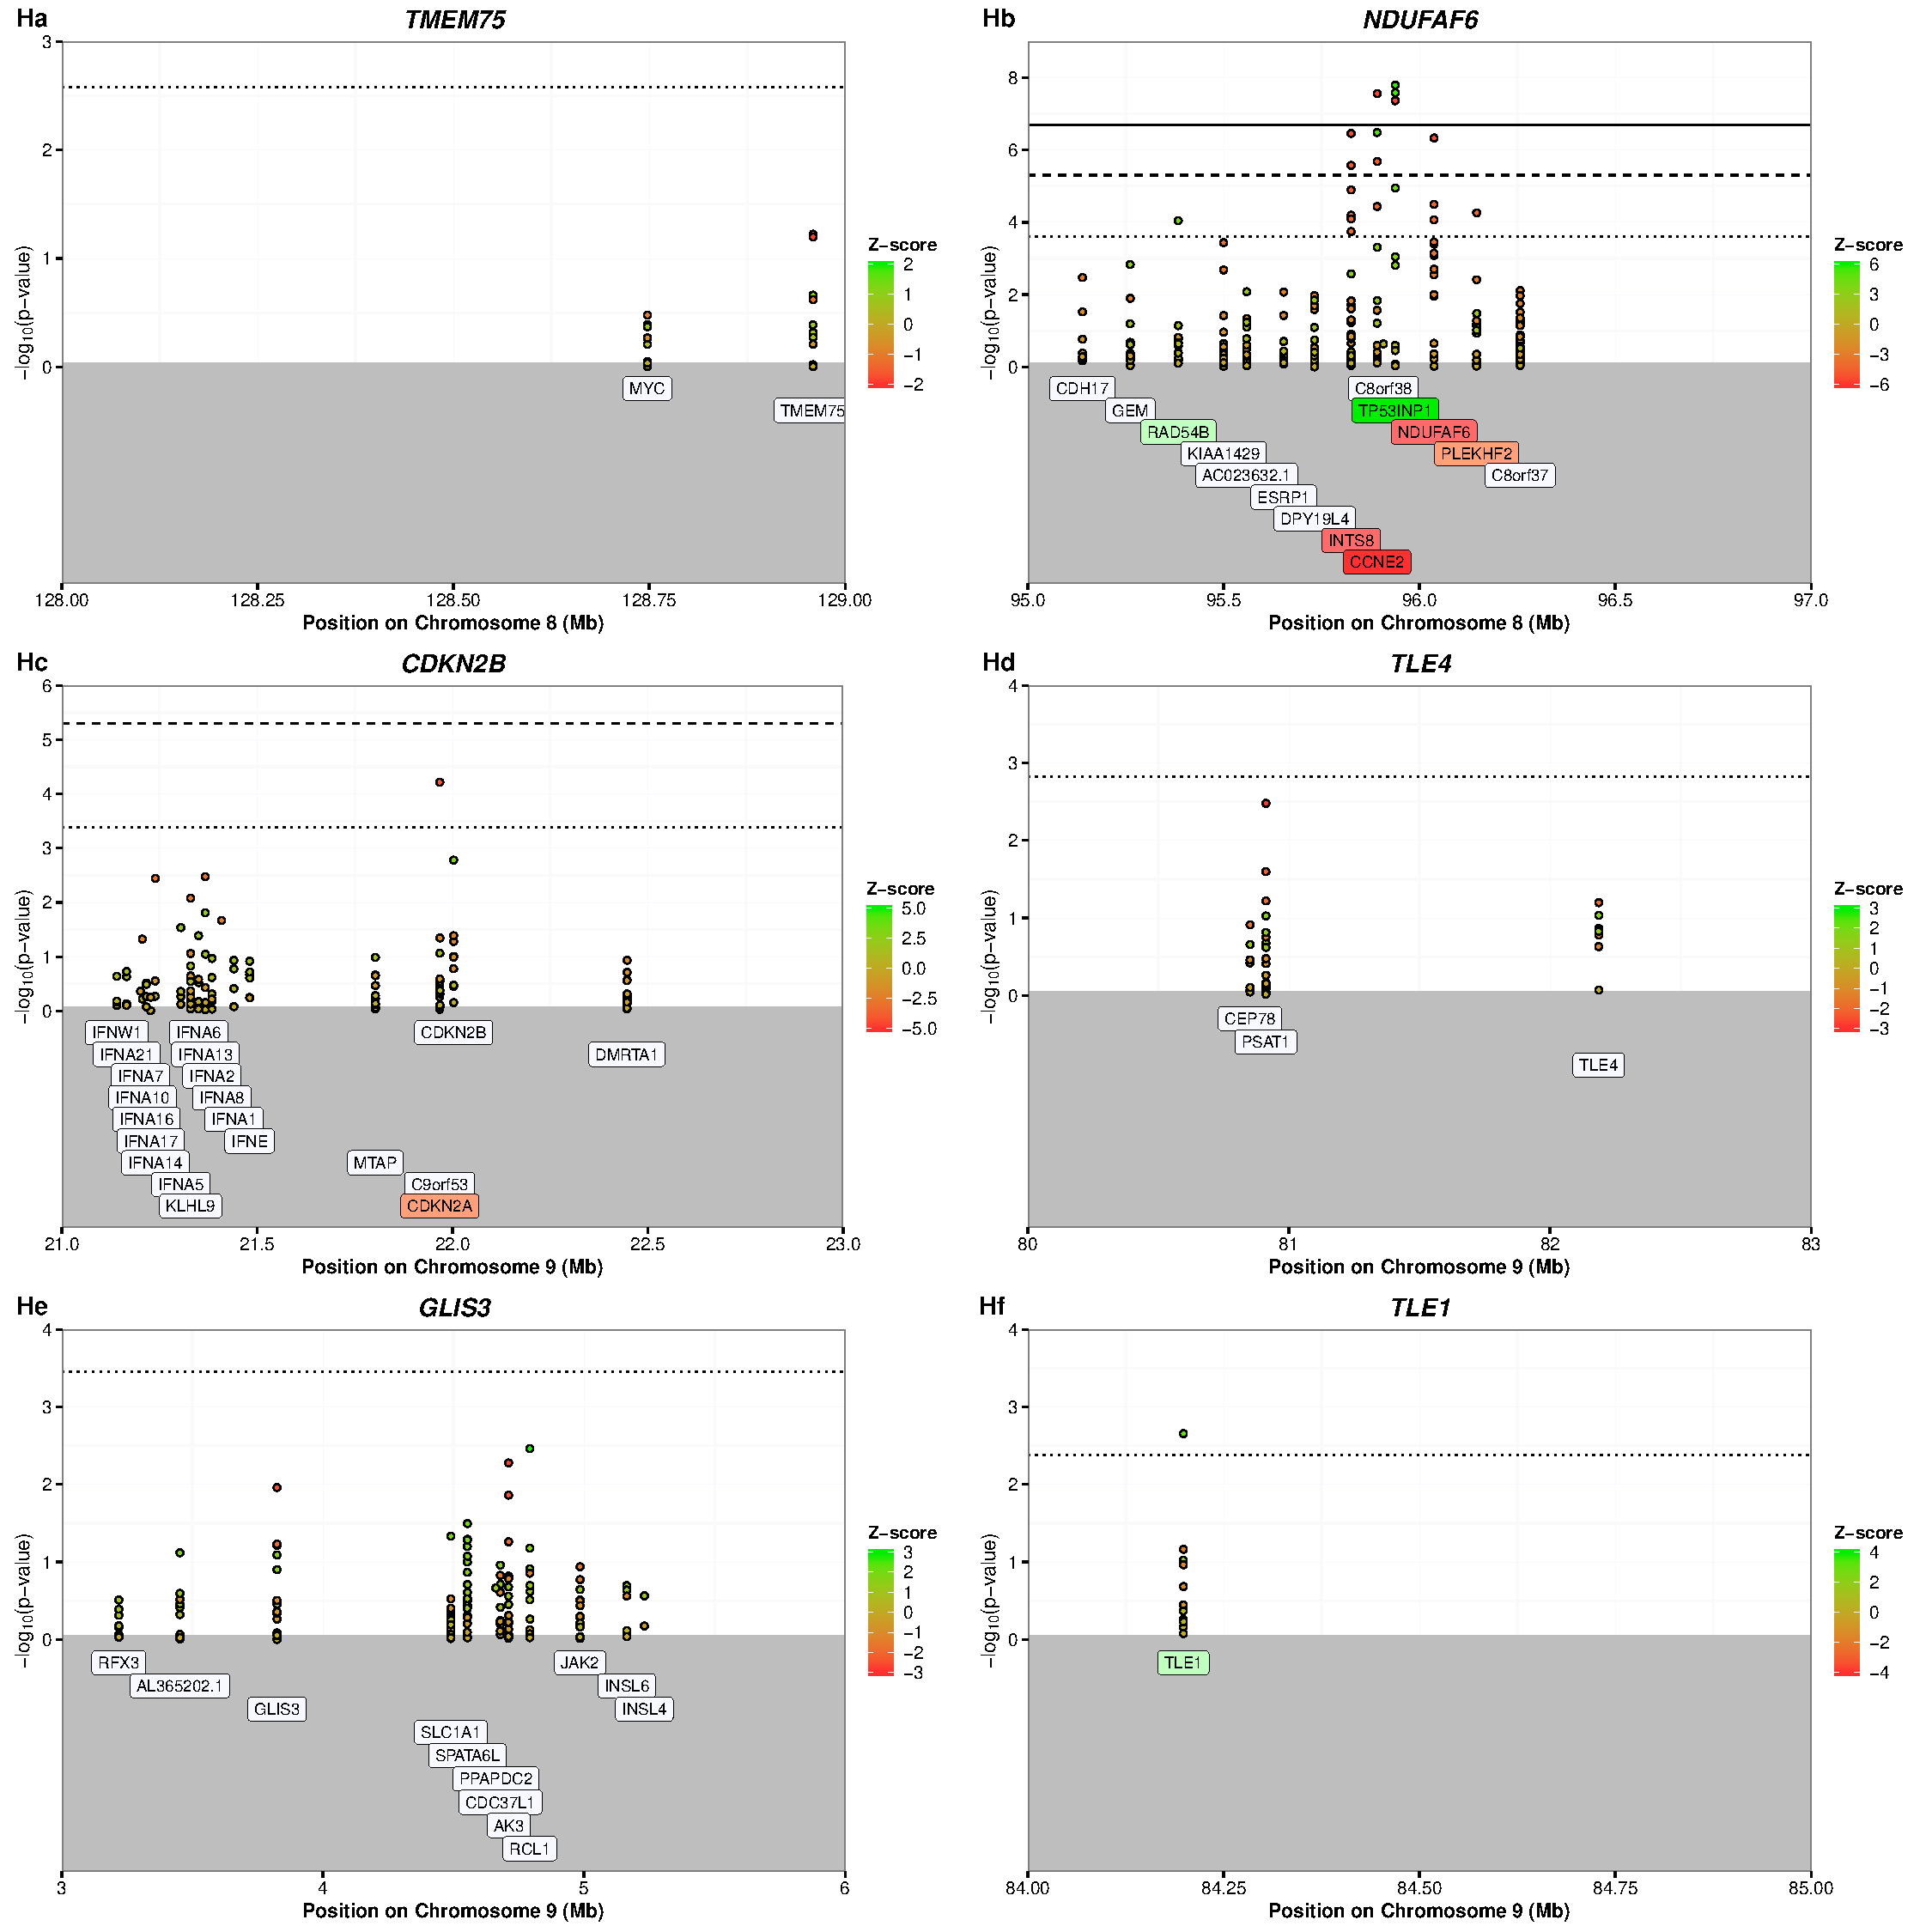
\includegraphics[width=\textwidth]{sup_fig1_part8_locusArray.pdf}
	\caption{\textbf{MetaXcan profiles at T2D-associated loci} We tested for association between predicted gene expression and T2D at $\sim2$ Mb genomic regions encompassing putative T2D genes implicated by the top $1,000$ SNPs associated with T2D from the DIAGRAM trans-ethnic meta-analysis of GWASs using $42$ tissue-level prediction models. The gene about which the genomic region is centered is indicated at the top of each panel. The solid, dashed, and dotted line denote significance correcting for the total number of tests performed across all models, genome-wide significance in a single model ($10,000$ tests), and locus-wide significance, respectively. Genomic position (Mb) and significance ($-\log_{10}$(p-value)) for each predicted gene expression value (from a particular tissue model) are shown on the $x$ and $y$-axis, respectively. Gene labels are shown in the gray region and are positioned at the transcription start site (TSS). Moreover, color corresponds to the magnitude and sign of the $Z$-score where positive and negative $Z$-scores are colored green and red, respectively.} 
    \label{fig:supp.locus_array_fig1_part8}
\end{figure}

\begin{figure}
\ContinuedFloat
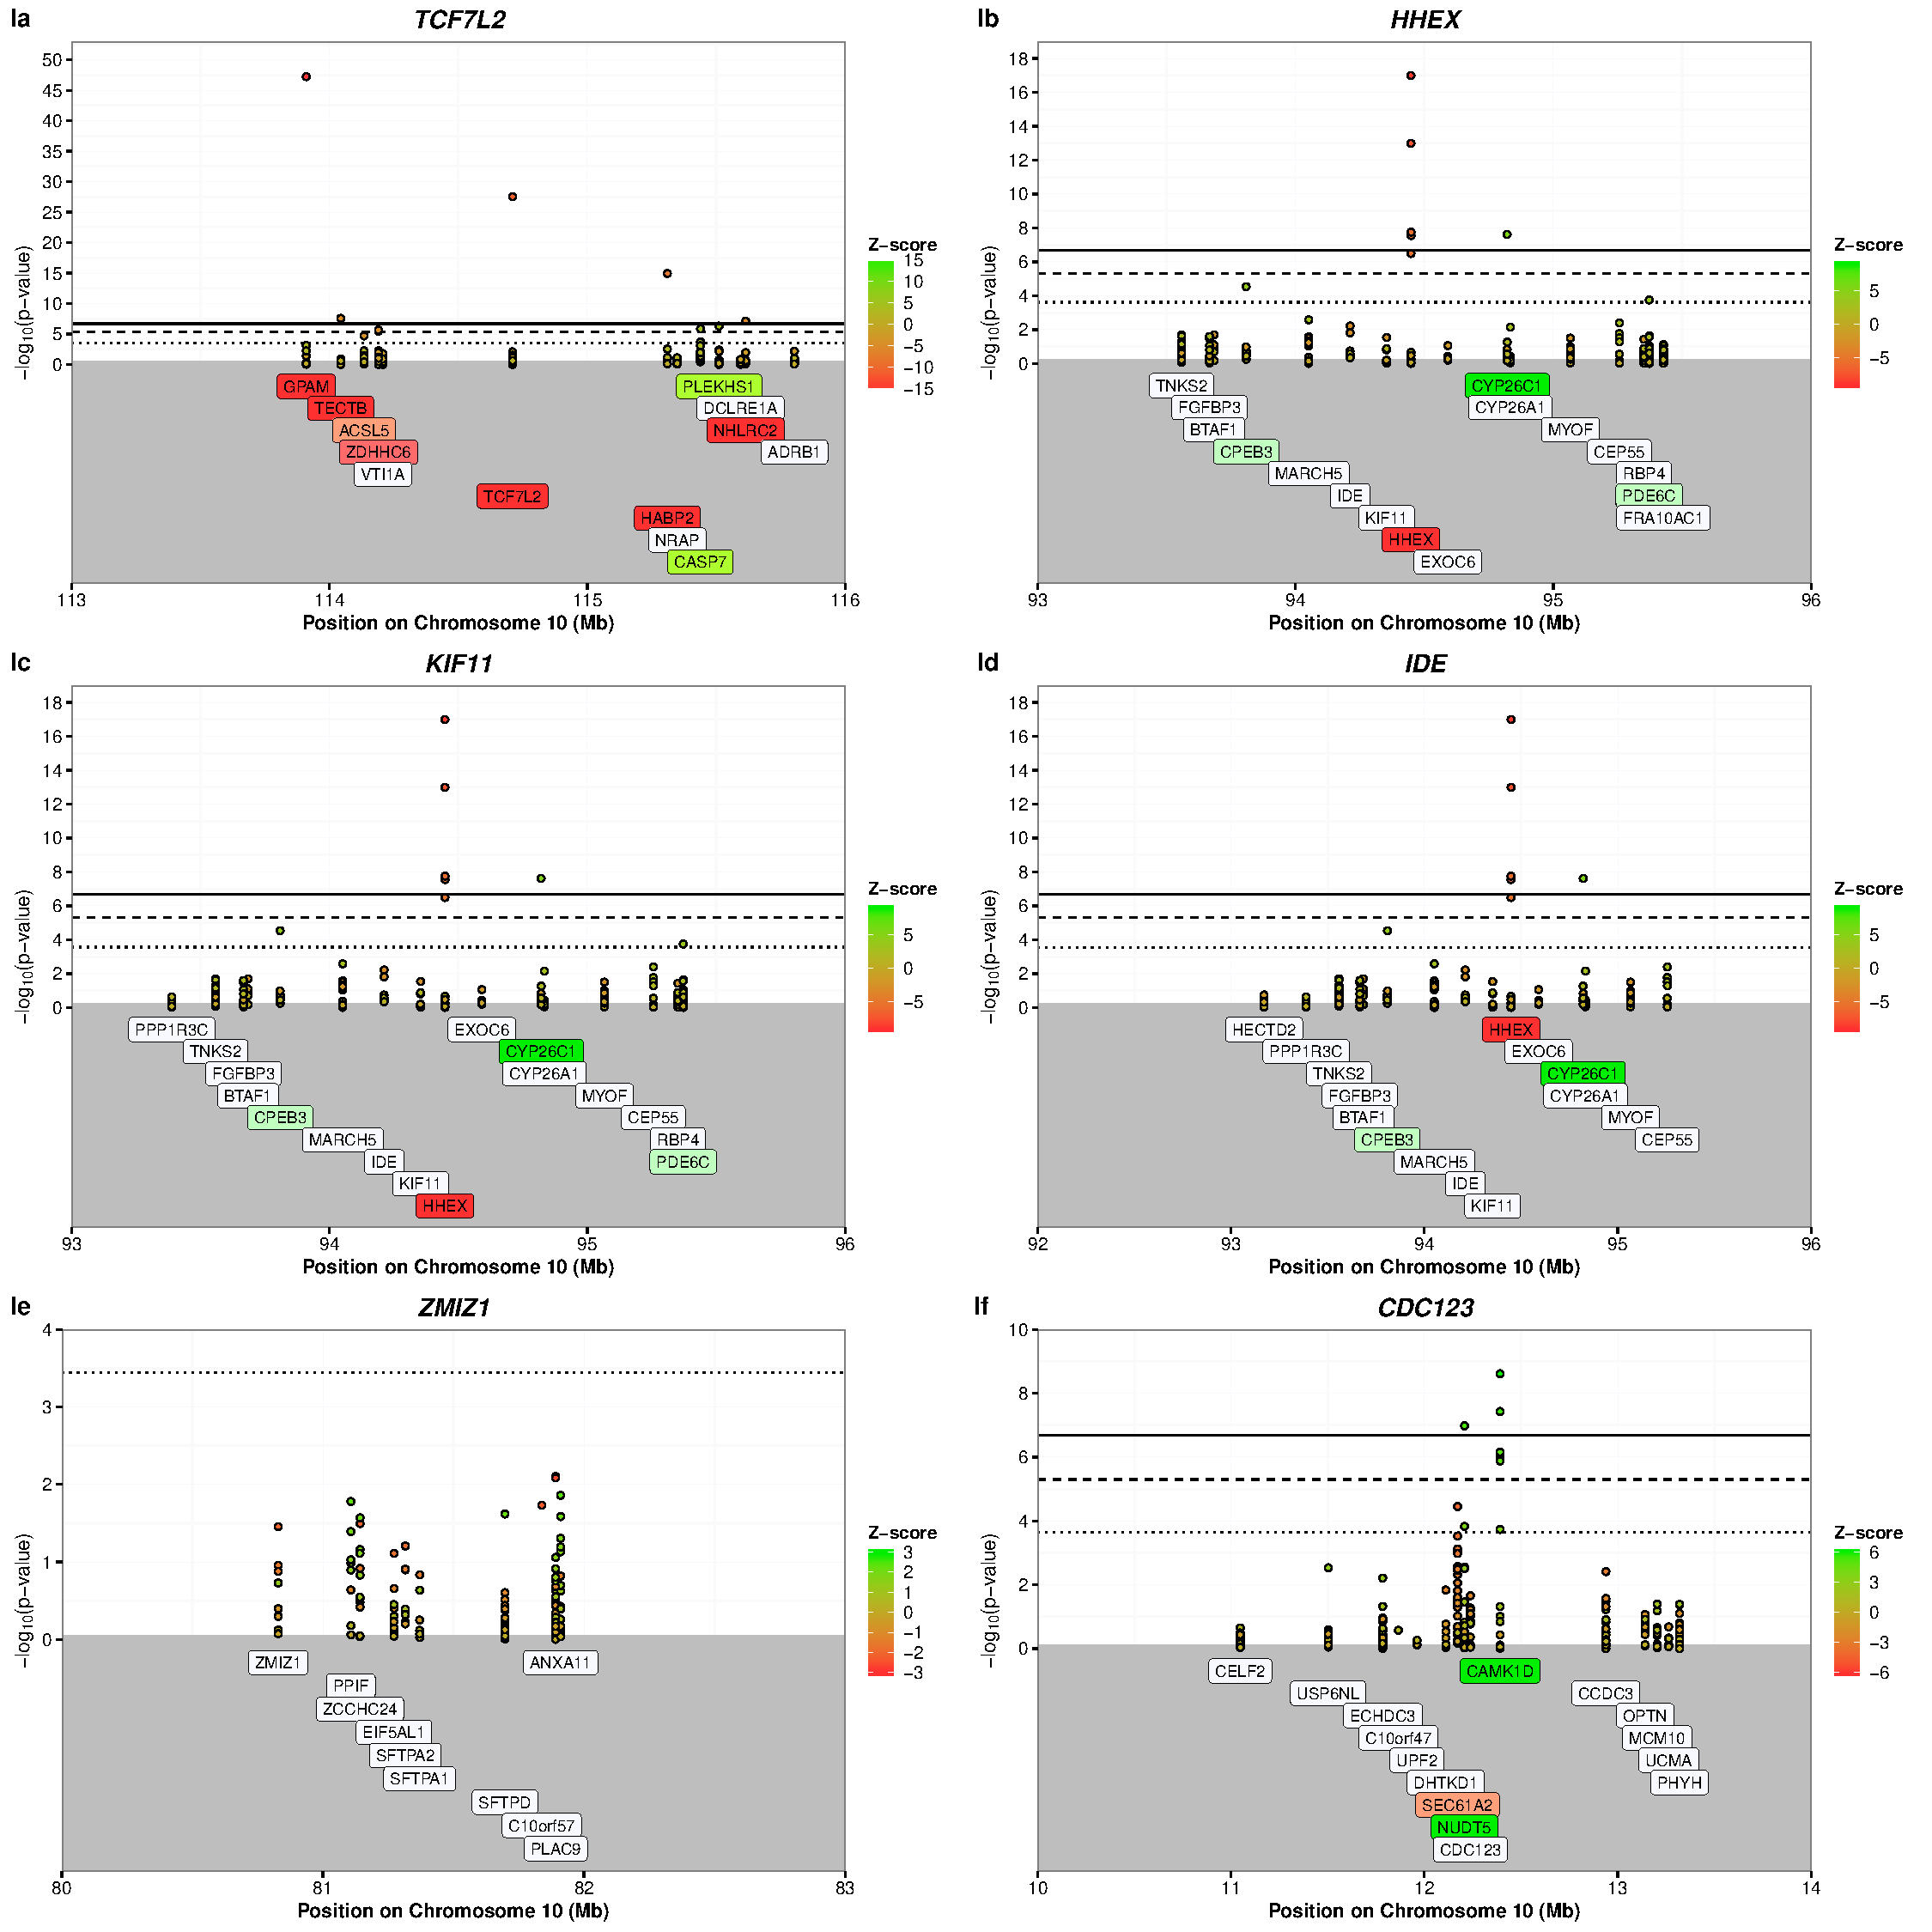
\includegraphics[width=\textwidth]{sup_fig1_part9_locusArray.pdf}
	\caption{\textbf{MetaXcan profiles at T2D-associated loci} We tested for association between predicted gene expression and T2D at $\sim2$ Mb genomic regions encompassing putative T2D genes implicated by the top $1,000$ SNPs associated with T2D from the DIAGRAM trans-ethnic meta-analysis of GWASs using $42$ tissue-level prediction models. The gene about which the genomic region is centered is indicated at the top of each panel. The solid, dashed, and dotted line denote significance correcting for the total number of tests performed across all models, genome-wide significance in a single model ($10,000$ tests), and locus-wide significance, respectively. Genomic position (Mb) and significance ($-\log_{10}$(p-value)) for each predicted gene expression value (from a particular tissue model) are shown on the $x$ and $y$-axis, respectively. Gene labels are shown in the gray region and are positioned at the transcription start site (TSS). Moreover, color corresponds to the magnitude and sign of the $Z$-score where positive and negative $Z$-scores are colored green and red, respectively.} 
    \label{fig:supp.locus_array_fig1_part9}
\end{figure}

\begin{figure}
\ContinuedFloat
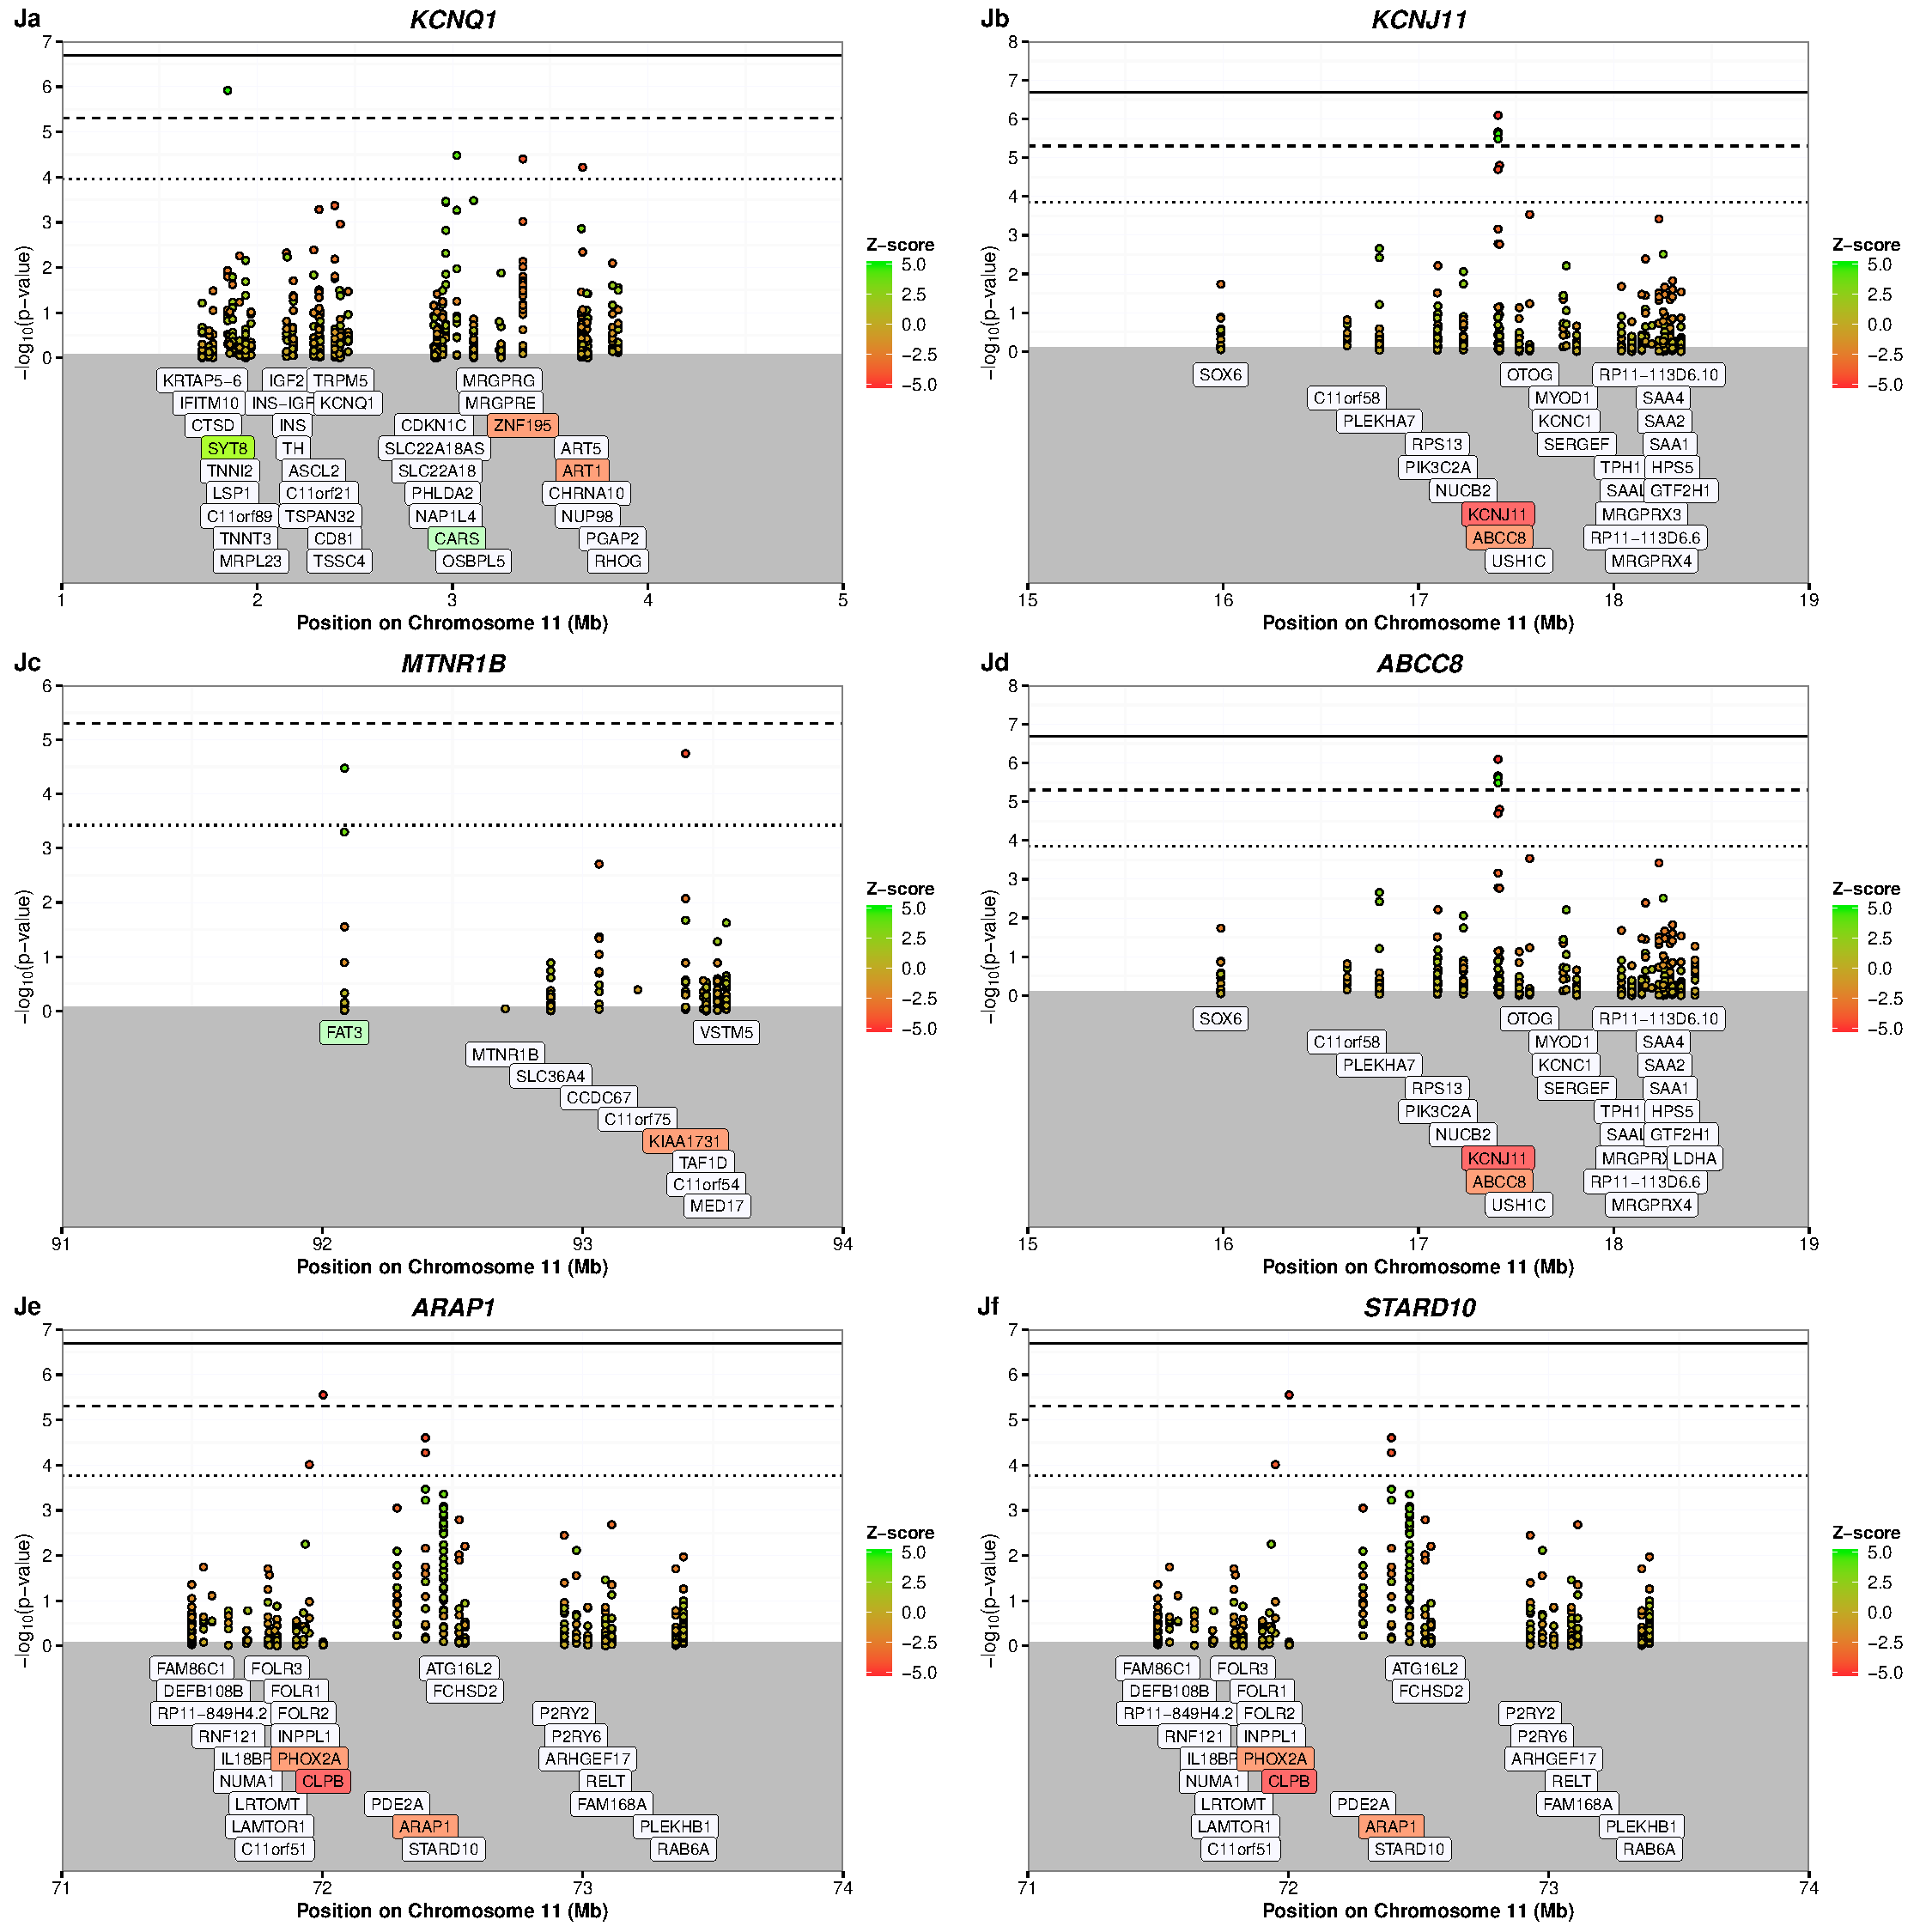
\includegraphics[width=\textwidth]{sup_fig1_part10_locusArray.pdf}
	\caption{\textbf{MetaXcan profiles at T2D-associated loci} We tested for association between predicted gene expression and T2D at $\sim2$ Mb genomic regions encompassing putative T2D genes implicated by the top $1,000$ SNPs associated with T2D from the DIAGRAM trans-ethnic meta-analysis of GWASs using $42$ tissue-level prediction models. The gene about which the genomic region is centered is indicated at the top of each panel. The solid, dashed, and dotted line denote significance correcting for the total number of tests performed across all models, genome-wide significance in a single model ($10,000$ tests), and locus-wide significance, respectively. Genomic position (Mb) and significance ($-\log_{10}$(p-value)) for each predicted gene expression value (from a particular tissue model) are shown on the $x$ and $y$-axis, respectively. Gene labels are shown in the gray region and are positioned at the transcription start site (TSS). Moreover, color corresponds to the magnitude and sign of the $Z$-score where positive and negative $Z$-scores are colored green and red, respectively.} 
    \label{fig:supp.locus_array_fig1_part10}
\end{figure}

\begin{figure}
\ContinuedFloat
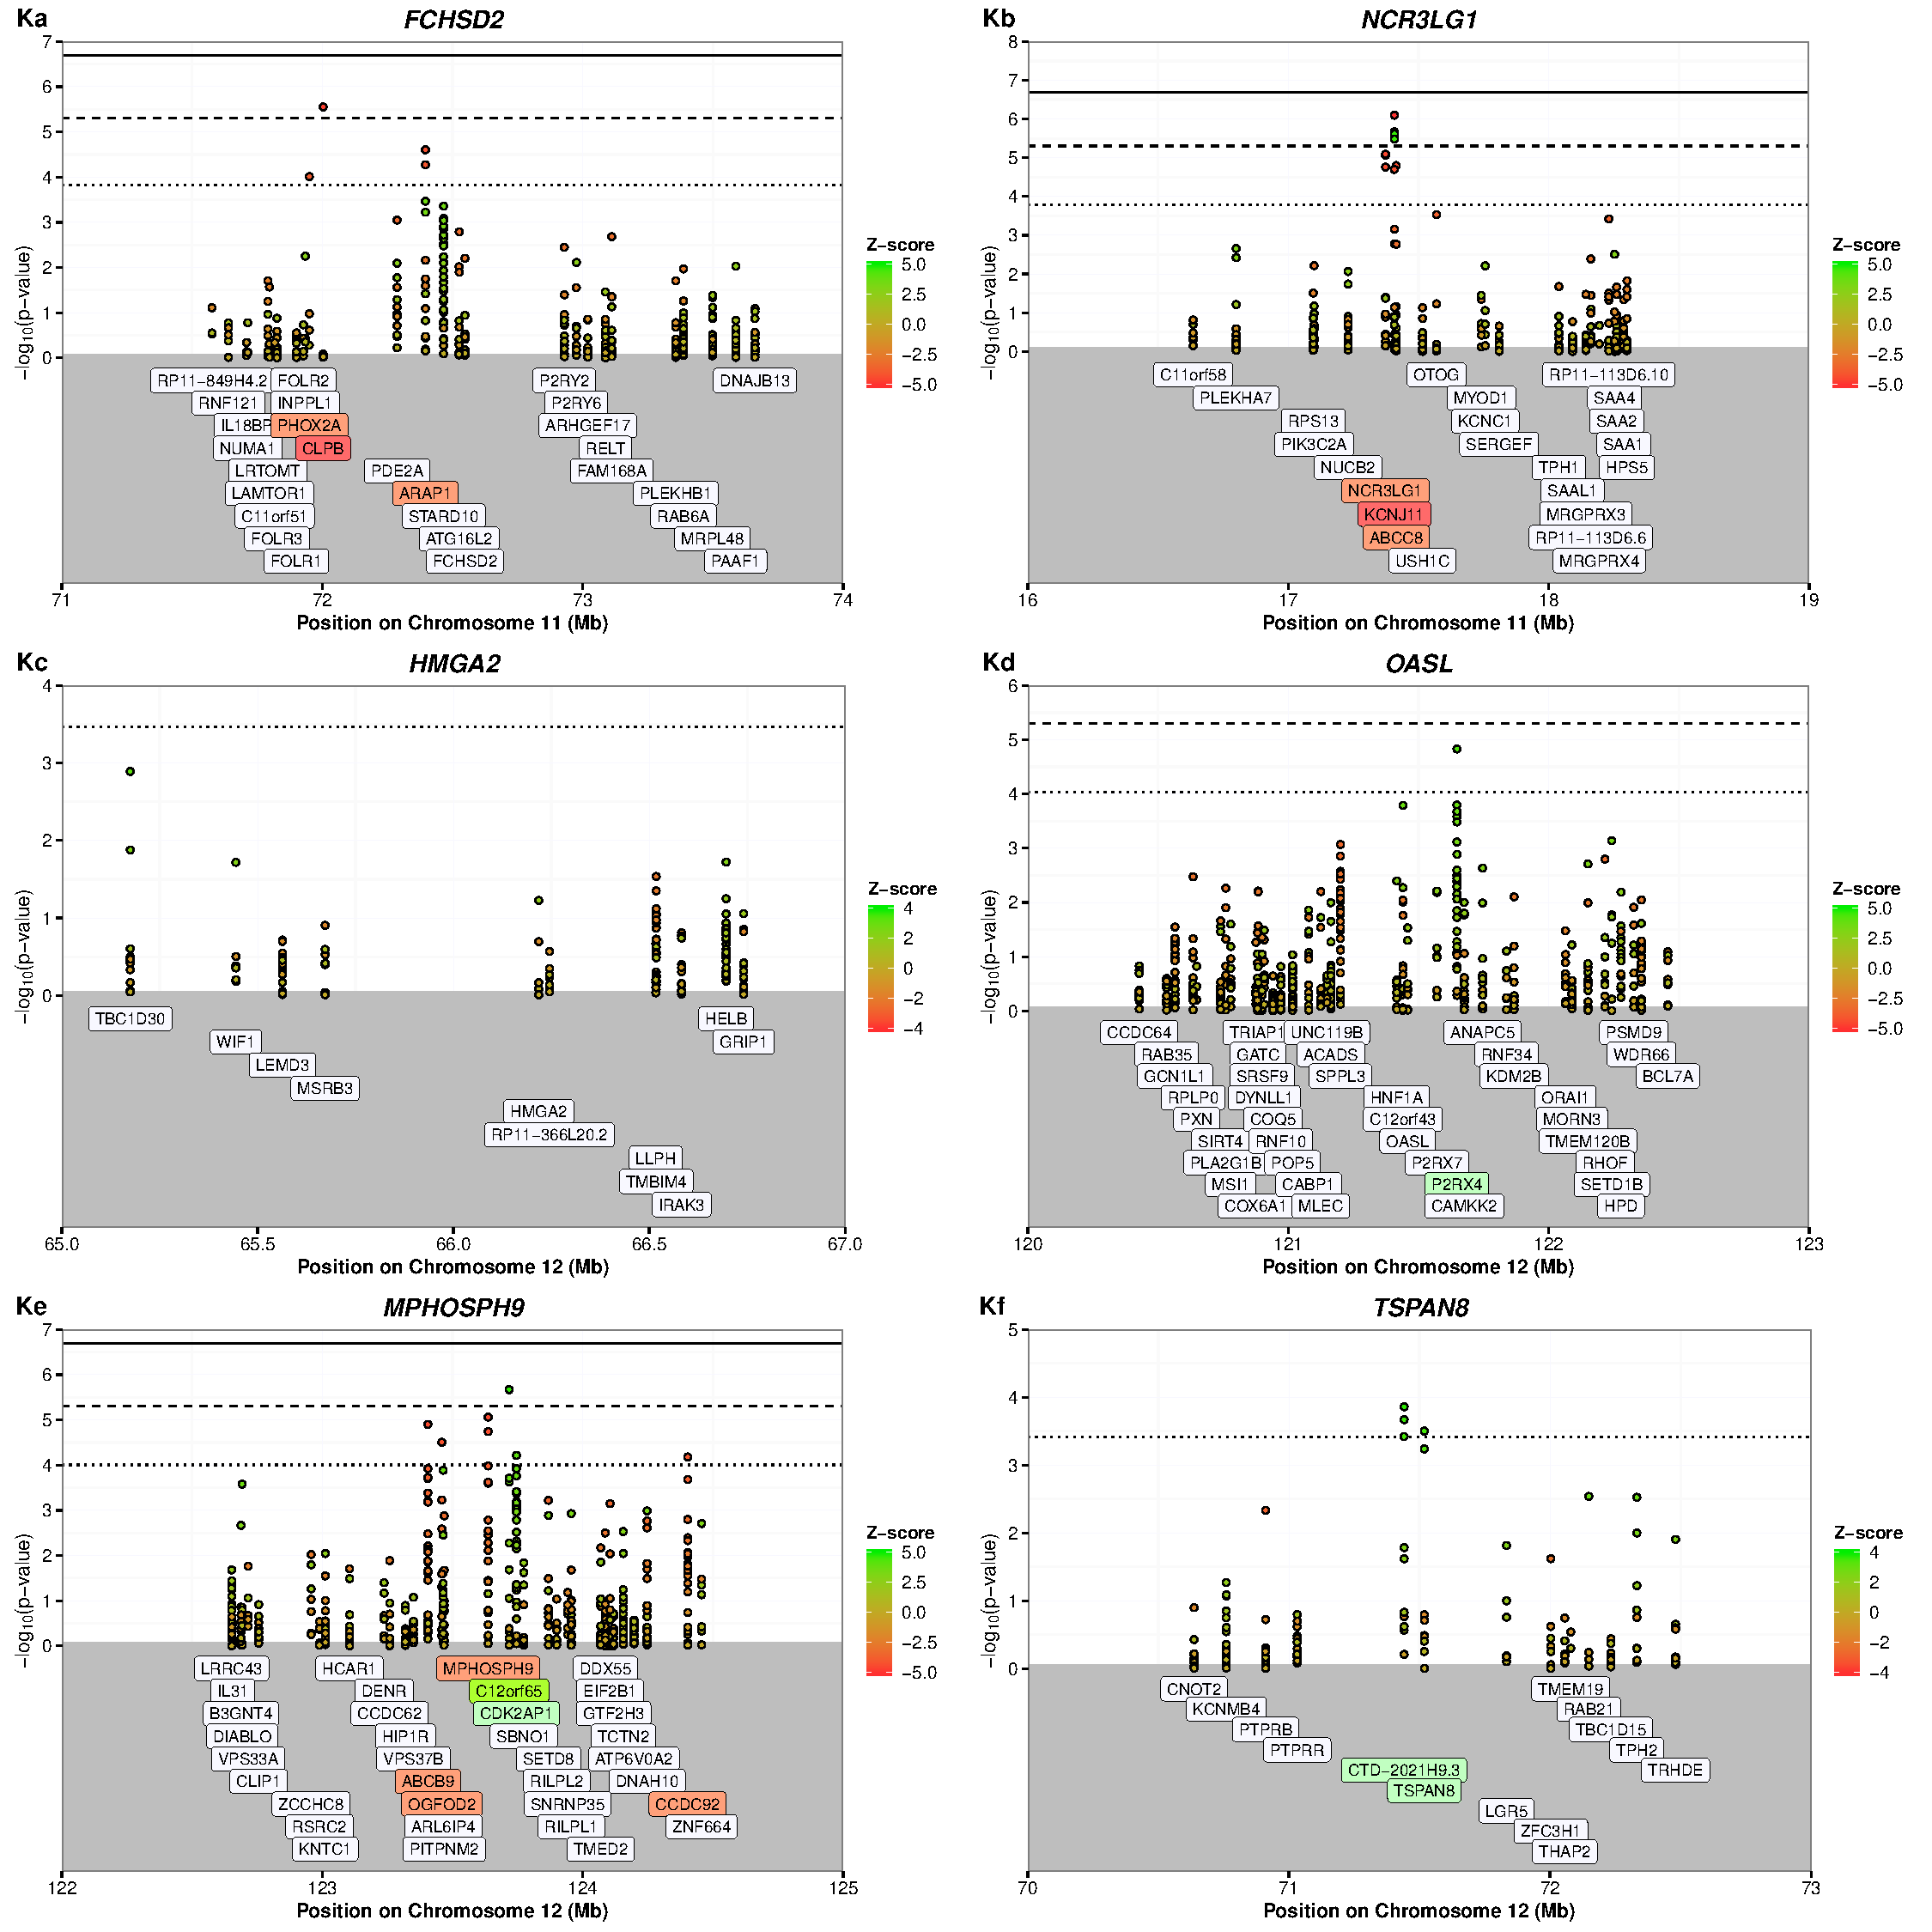
\includegraphics[width=\textwidth]{sup_fig1_part11_locusArray.pdf}
	\caption{\textbf{MetaXcan profiles at T2D-associated loci} We tested for association between predicted gene expression and T2D at $\sim2$ Mb genomic regions encompassing putative T2D genes implicated by the top $1,000$ SNPs associated with T2D from the DIAGRAM trans-ethnic meta-analysis of GWASs using $42$ tissue-level prediction models. The gene about which the genomic region is centered is indicated at the top of each panel. The solid, dashed, and dotted line denote significance correcting for the total number of tests performed across all models, genome-wide significance in a single model ($10,000$ tests), and locus-wide significance, respectively. Genomic position (Mb) and significance ($-\log_{10}$(p-value)) for each predicted gene expression value (from a particular tissue model) are shown on the $x$ and $y$-axis, respectively. Gene labels are shown in the gray region and are positioned at the transcription start site (TSS). Moreover, color corresponds to the magnitude and sign of the $Z$-score where positive and negative $Z$-scores are colored green and red, respectively.} 
    \label{fig:supp.locus_array_fig1_part11}
\end{figure}

\begin{figure}
\ContinuedFloat
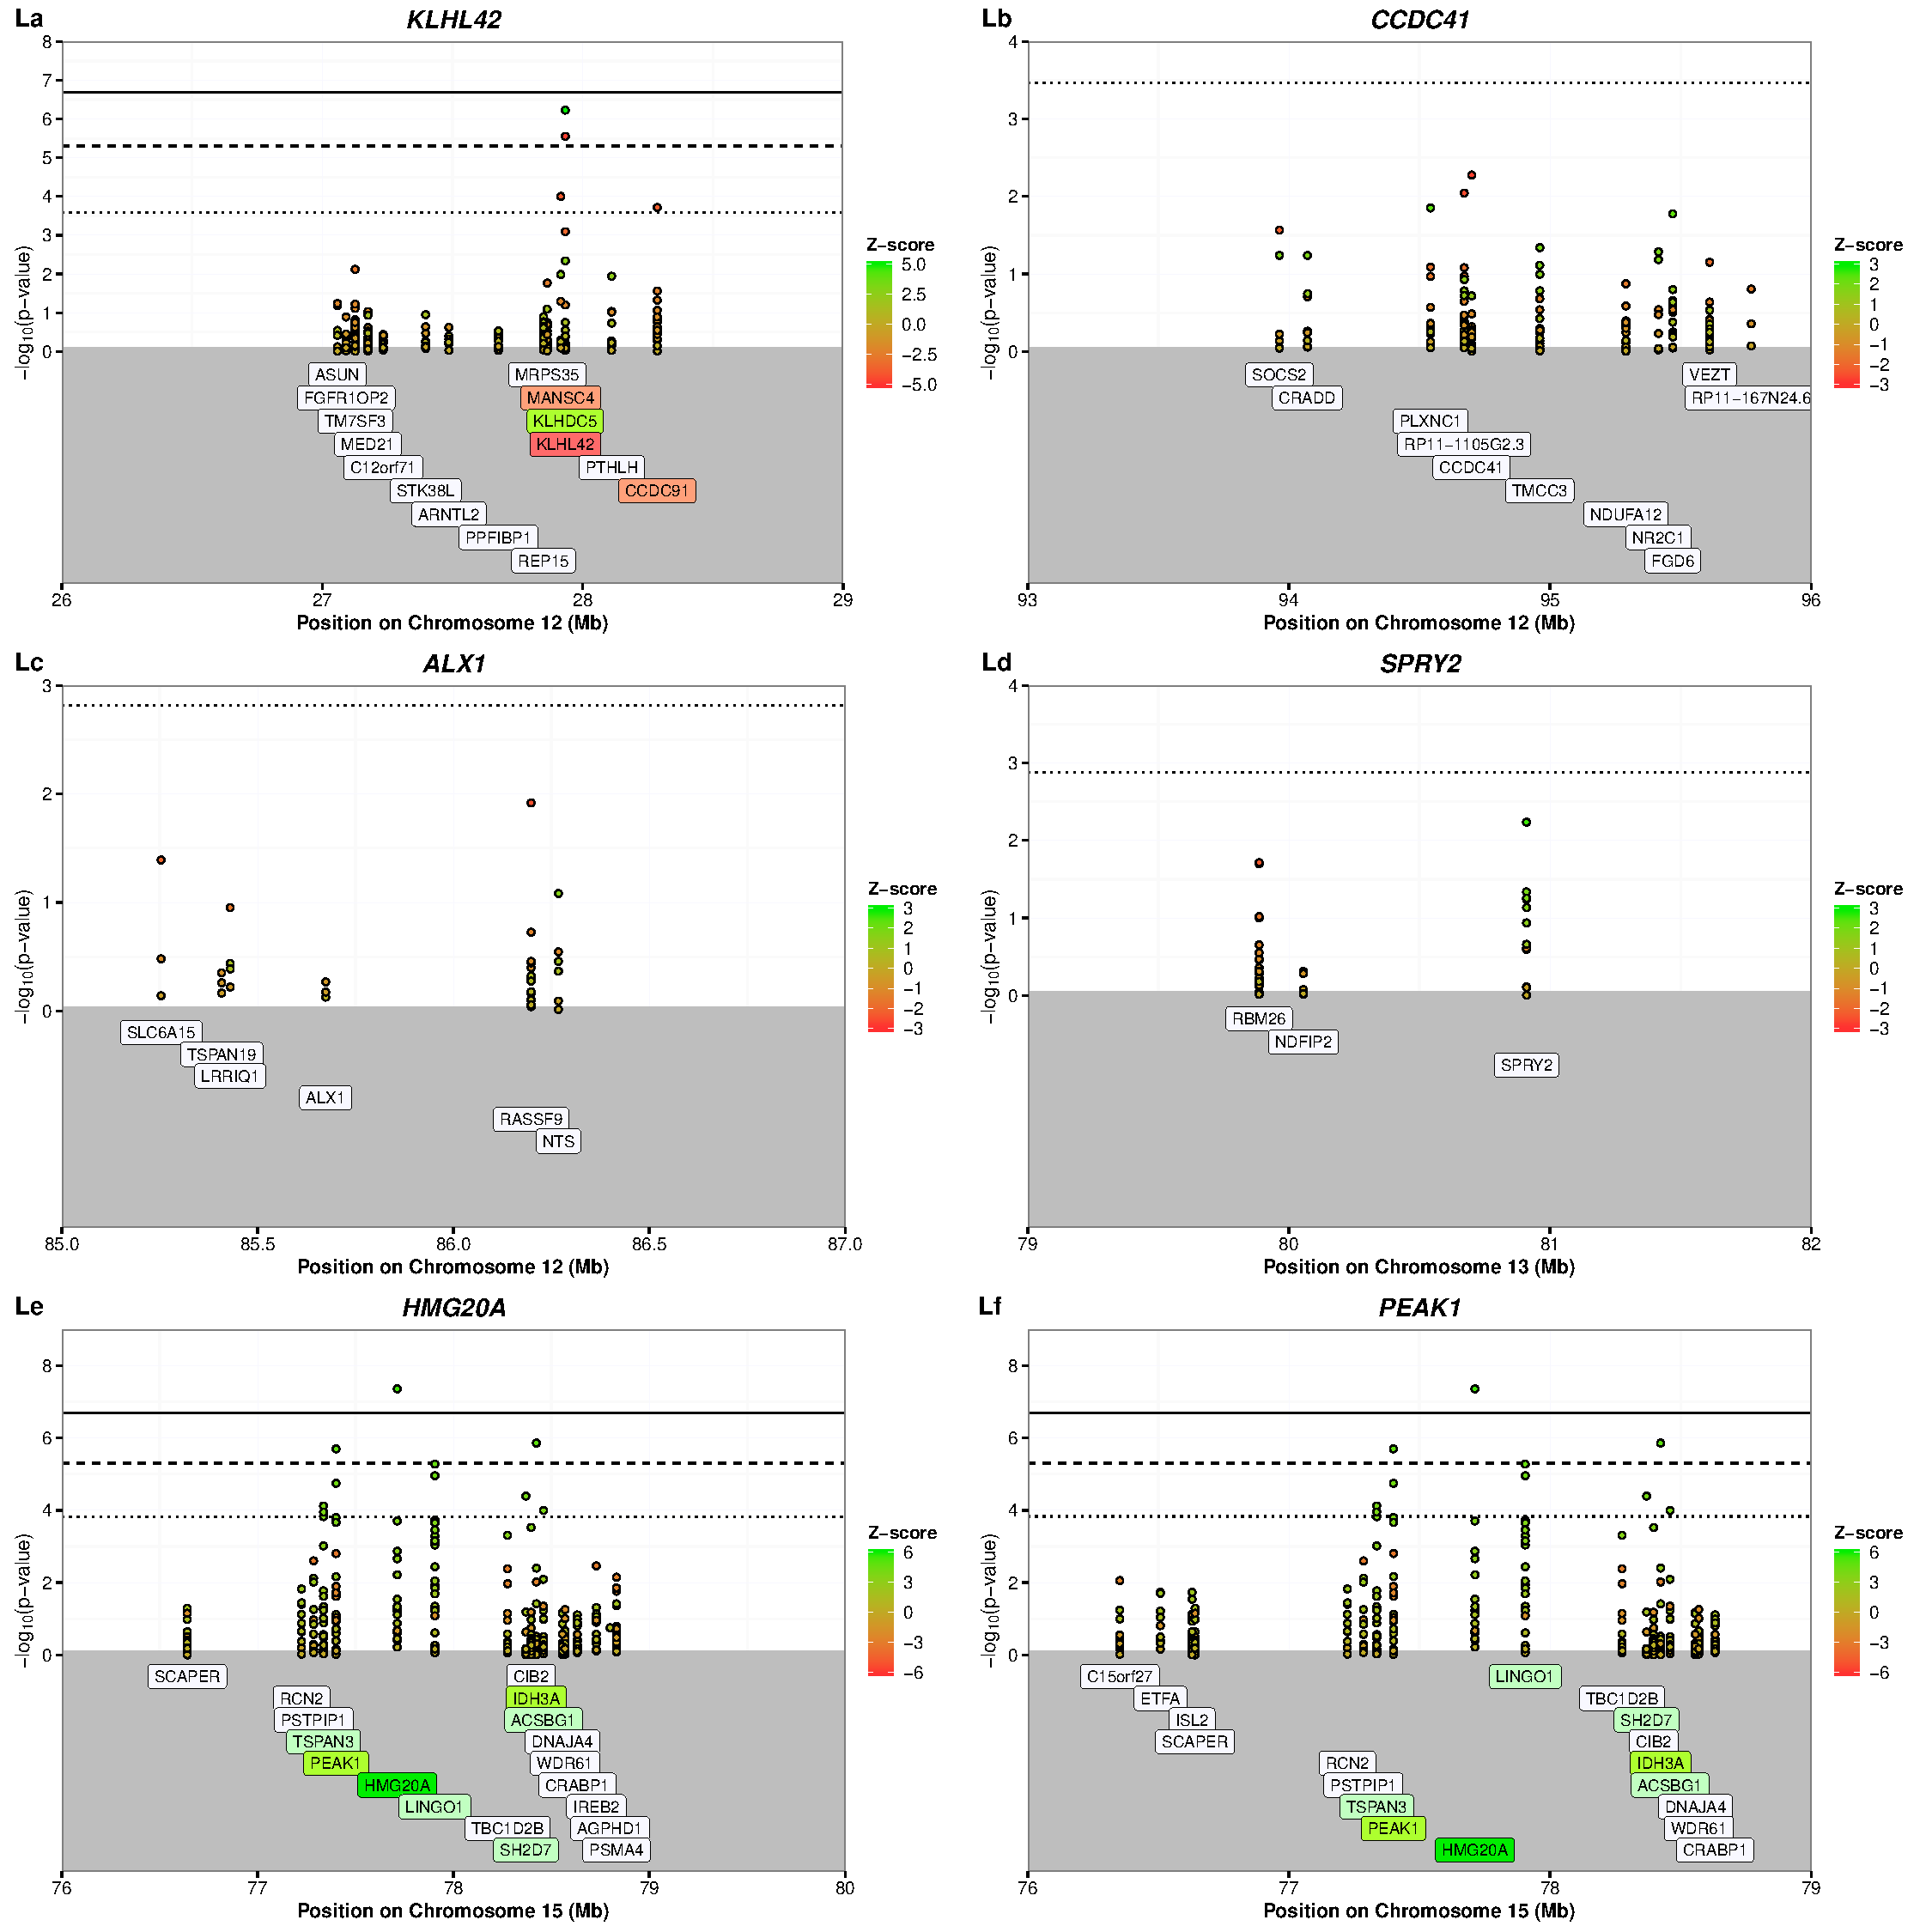
\includegraphics[width=\textwidth]{sup_fig1_part12_locusArray.pdf}
	\caption{\textbf{MetaXcan profiles at T2D-associated loci} We tested for association between predicted gene expression and T2D at $\sim2$ Mb genomic regions encompassing putative T2D genes implicated by the top $1,000$ SNPs associated with T2D from the DIAGRAM trans-ethnic meta-analysis of GWASs using $42$ tissue-level prediction models. The gene about which the genomic region is centered is indicated at the top of each panel. The solid, dashed, and dotted line denote significance correcting for the total number of tests performed across all models, genome-wide significance in a single model ($10,000$ tests), and locus-wide significance, respectively. Genomic position (Mb) and significance ($-\log_{10}$(p-value)) for each predicted gene expression value (from a particular tissue model) are shown on the $x$ and $y$-axis, respectively. Gene labels are shown in the gray region and are positioned at the transcription start site (TSS). Moreover, color corresponds to the magnitude and sign of the $Z$-score where positive and negative $Z$-scores are colored green and red, respectively.} 
    \label{fig:supp.locus_array_fig1_part12}
\end{figure}

\begin{figure}
\ContinuedFloat
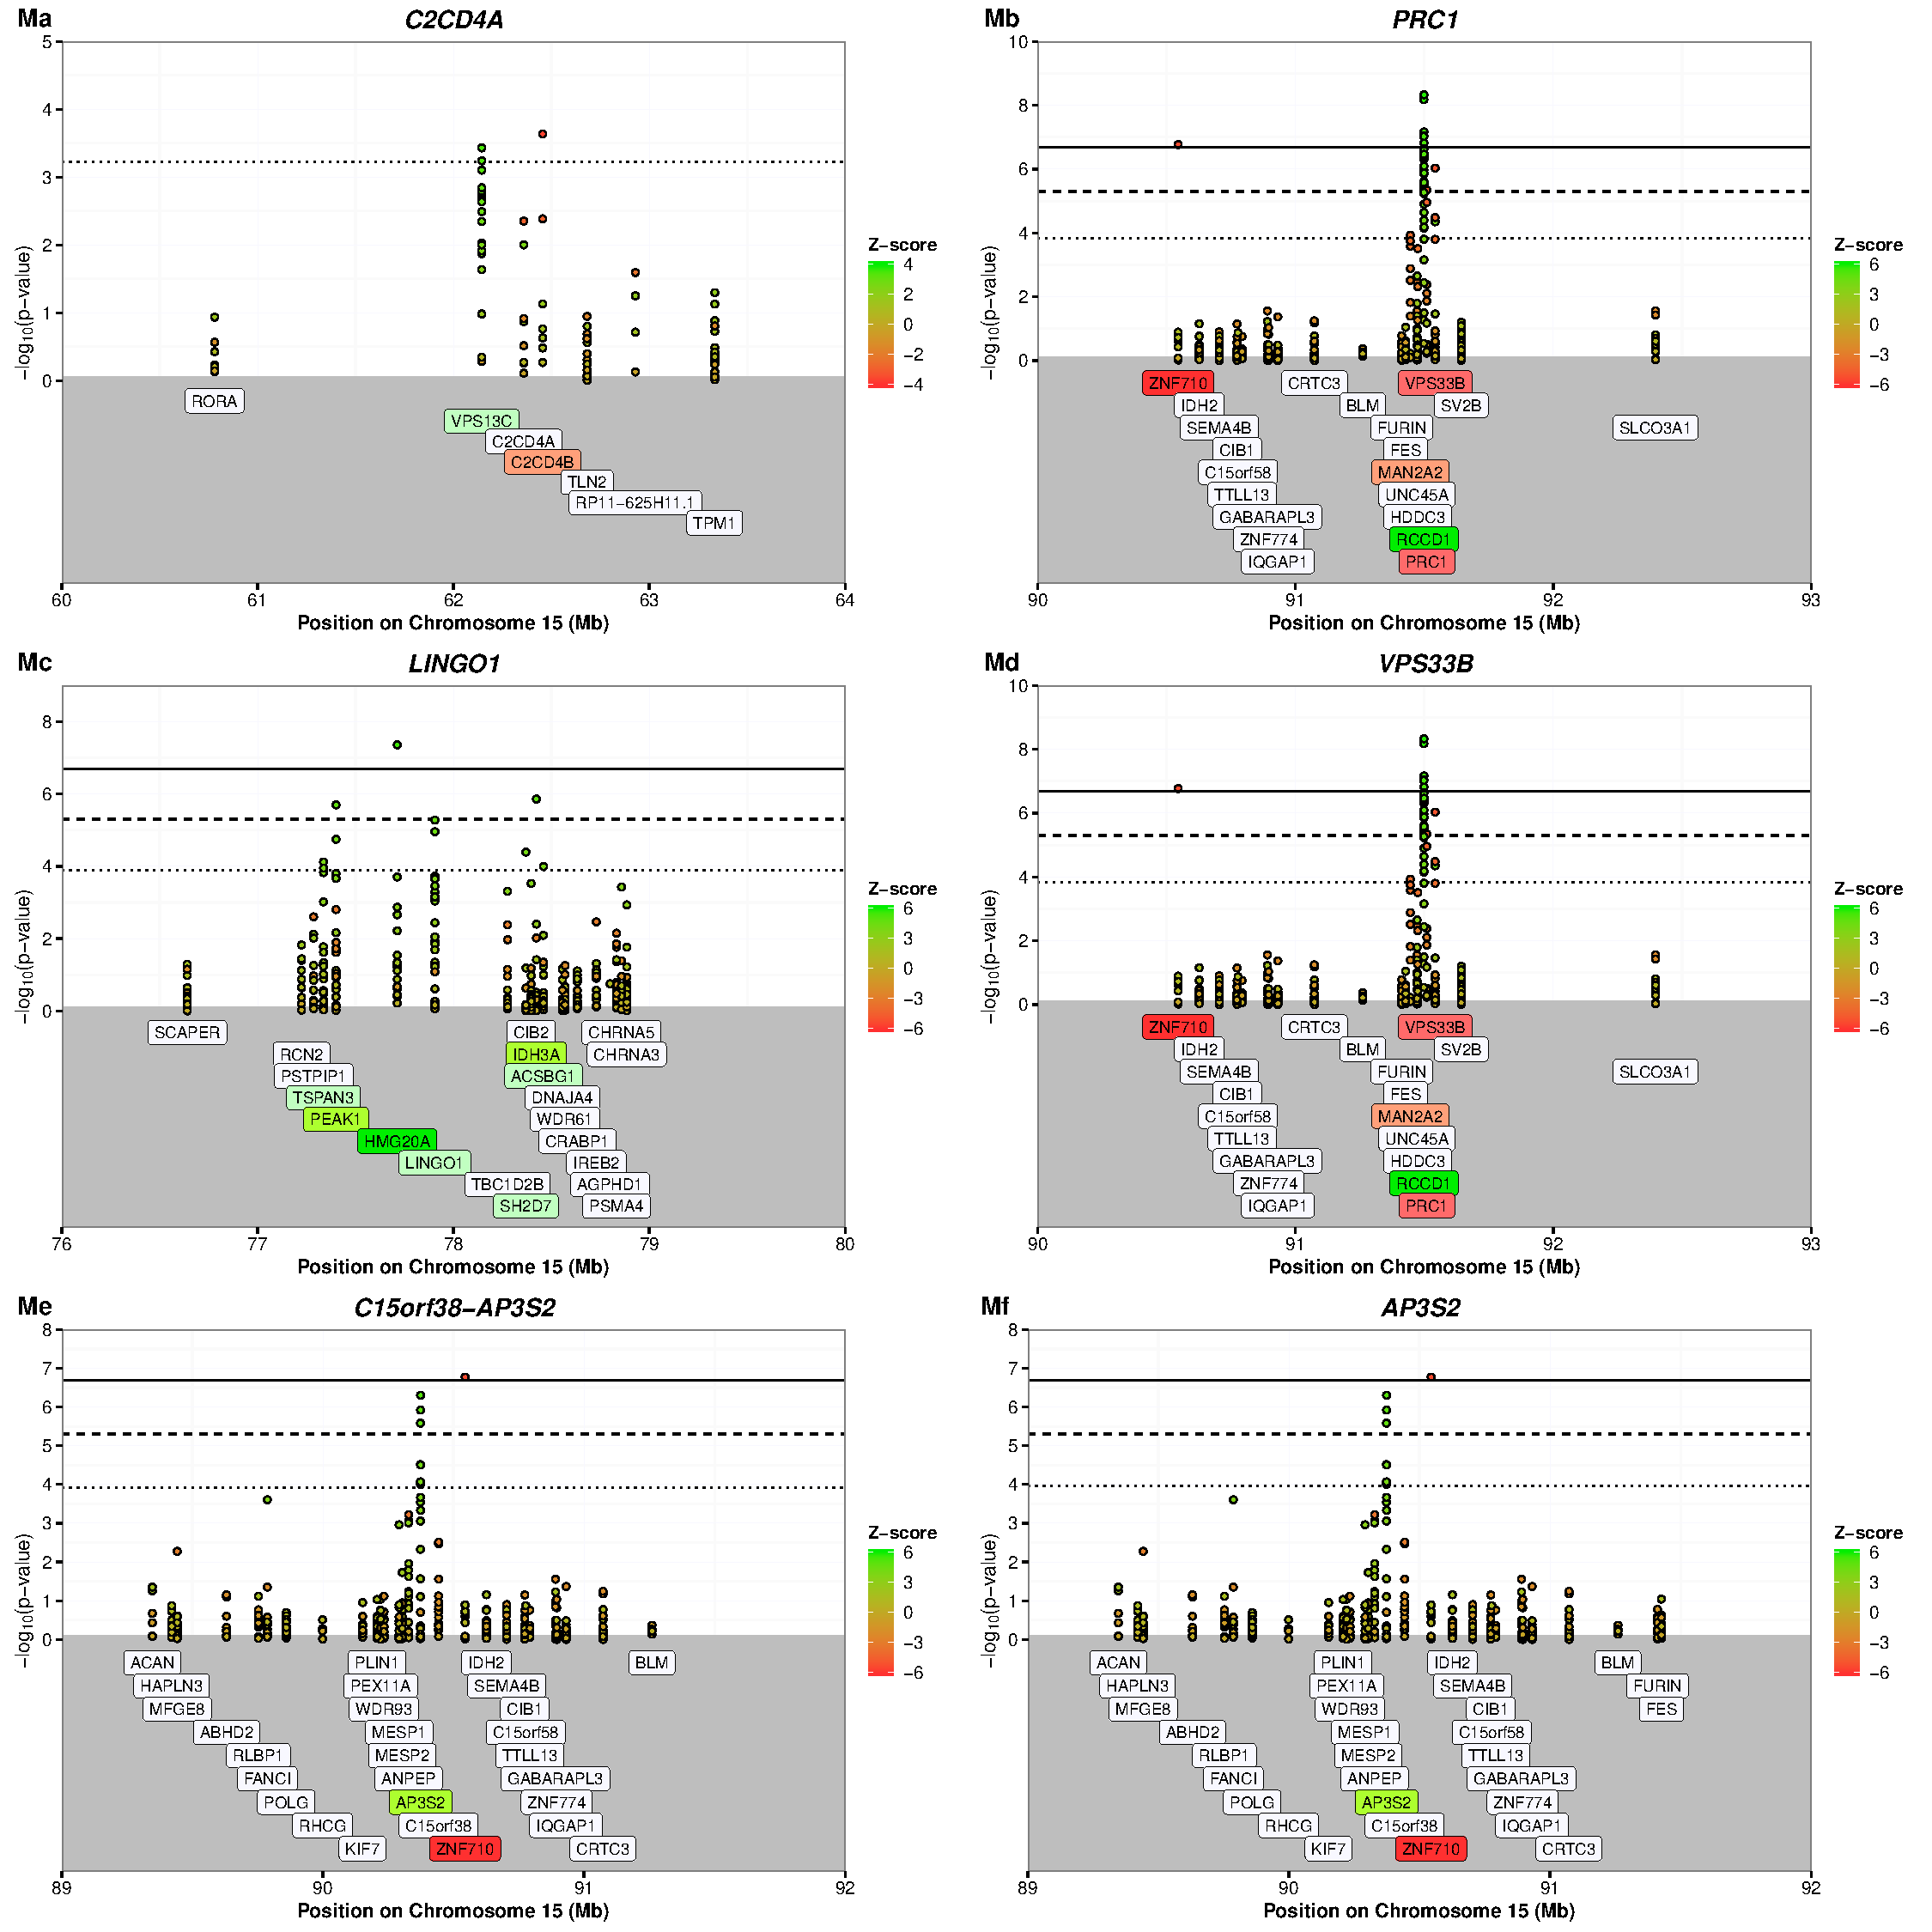
\includegraphics[width=\textwidth]{sup_fig1_part13_locusArray.pdf}
	\caption{\textbf{MetaXcan profiles at T2D-associated loci} We tested for association between predicted gene expression and T2D at $\sim2$ Mb genomic regions encompassing putative T2D genes implicated by the top $1,000$ SNPs associated with T2D from the DIAGRAM trans-ethnic meta-analysis of GWASs using $42$ tissue-level prediction models. The gene about which the genomic region is centered is indicated at the top of each panel. The solid, dashed, and dotted line denote significance correcting for the total number of tests performed across all models, genome-wide significance in a single model ($10,000$ tests), and locus-wide significance, respectively. Genomic position (Mb) and significance ($-\log_{10}$(p-value)) for each predicted gene expression value (from a particular tissue model) are shown on the $x$ and $y$-axis, respectively. Gene labels are shown in the gray region and are positioned at the transcription start site (TSS). Moreover, color corresponds to the magnitude and sign of the $Z$-score where positive and negative $Z$-scores are colored green and red, respectively.} 
    \label{fig:supp.locus_array_fig1_part13}
\end{figure}

\begin{figure}
\ContinuedFloat
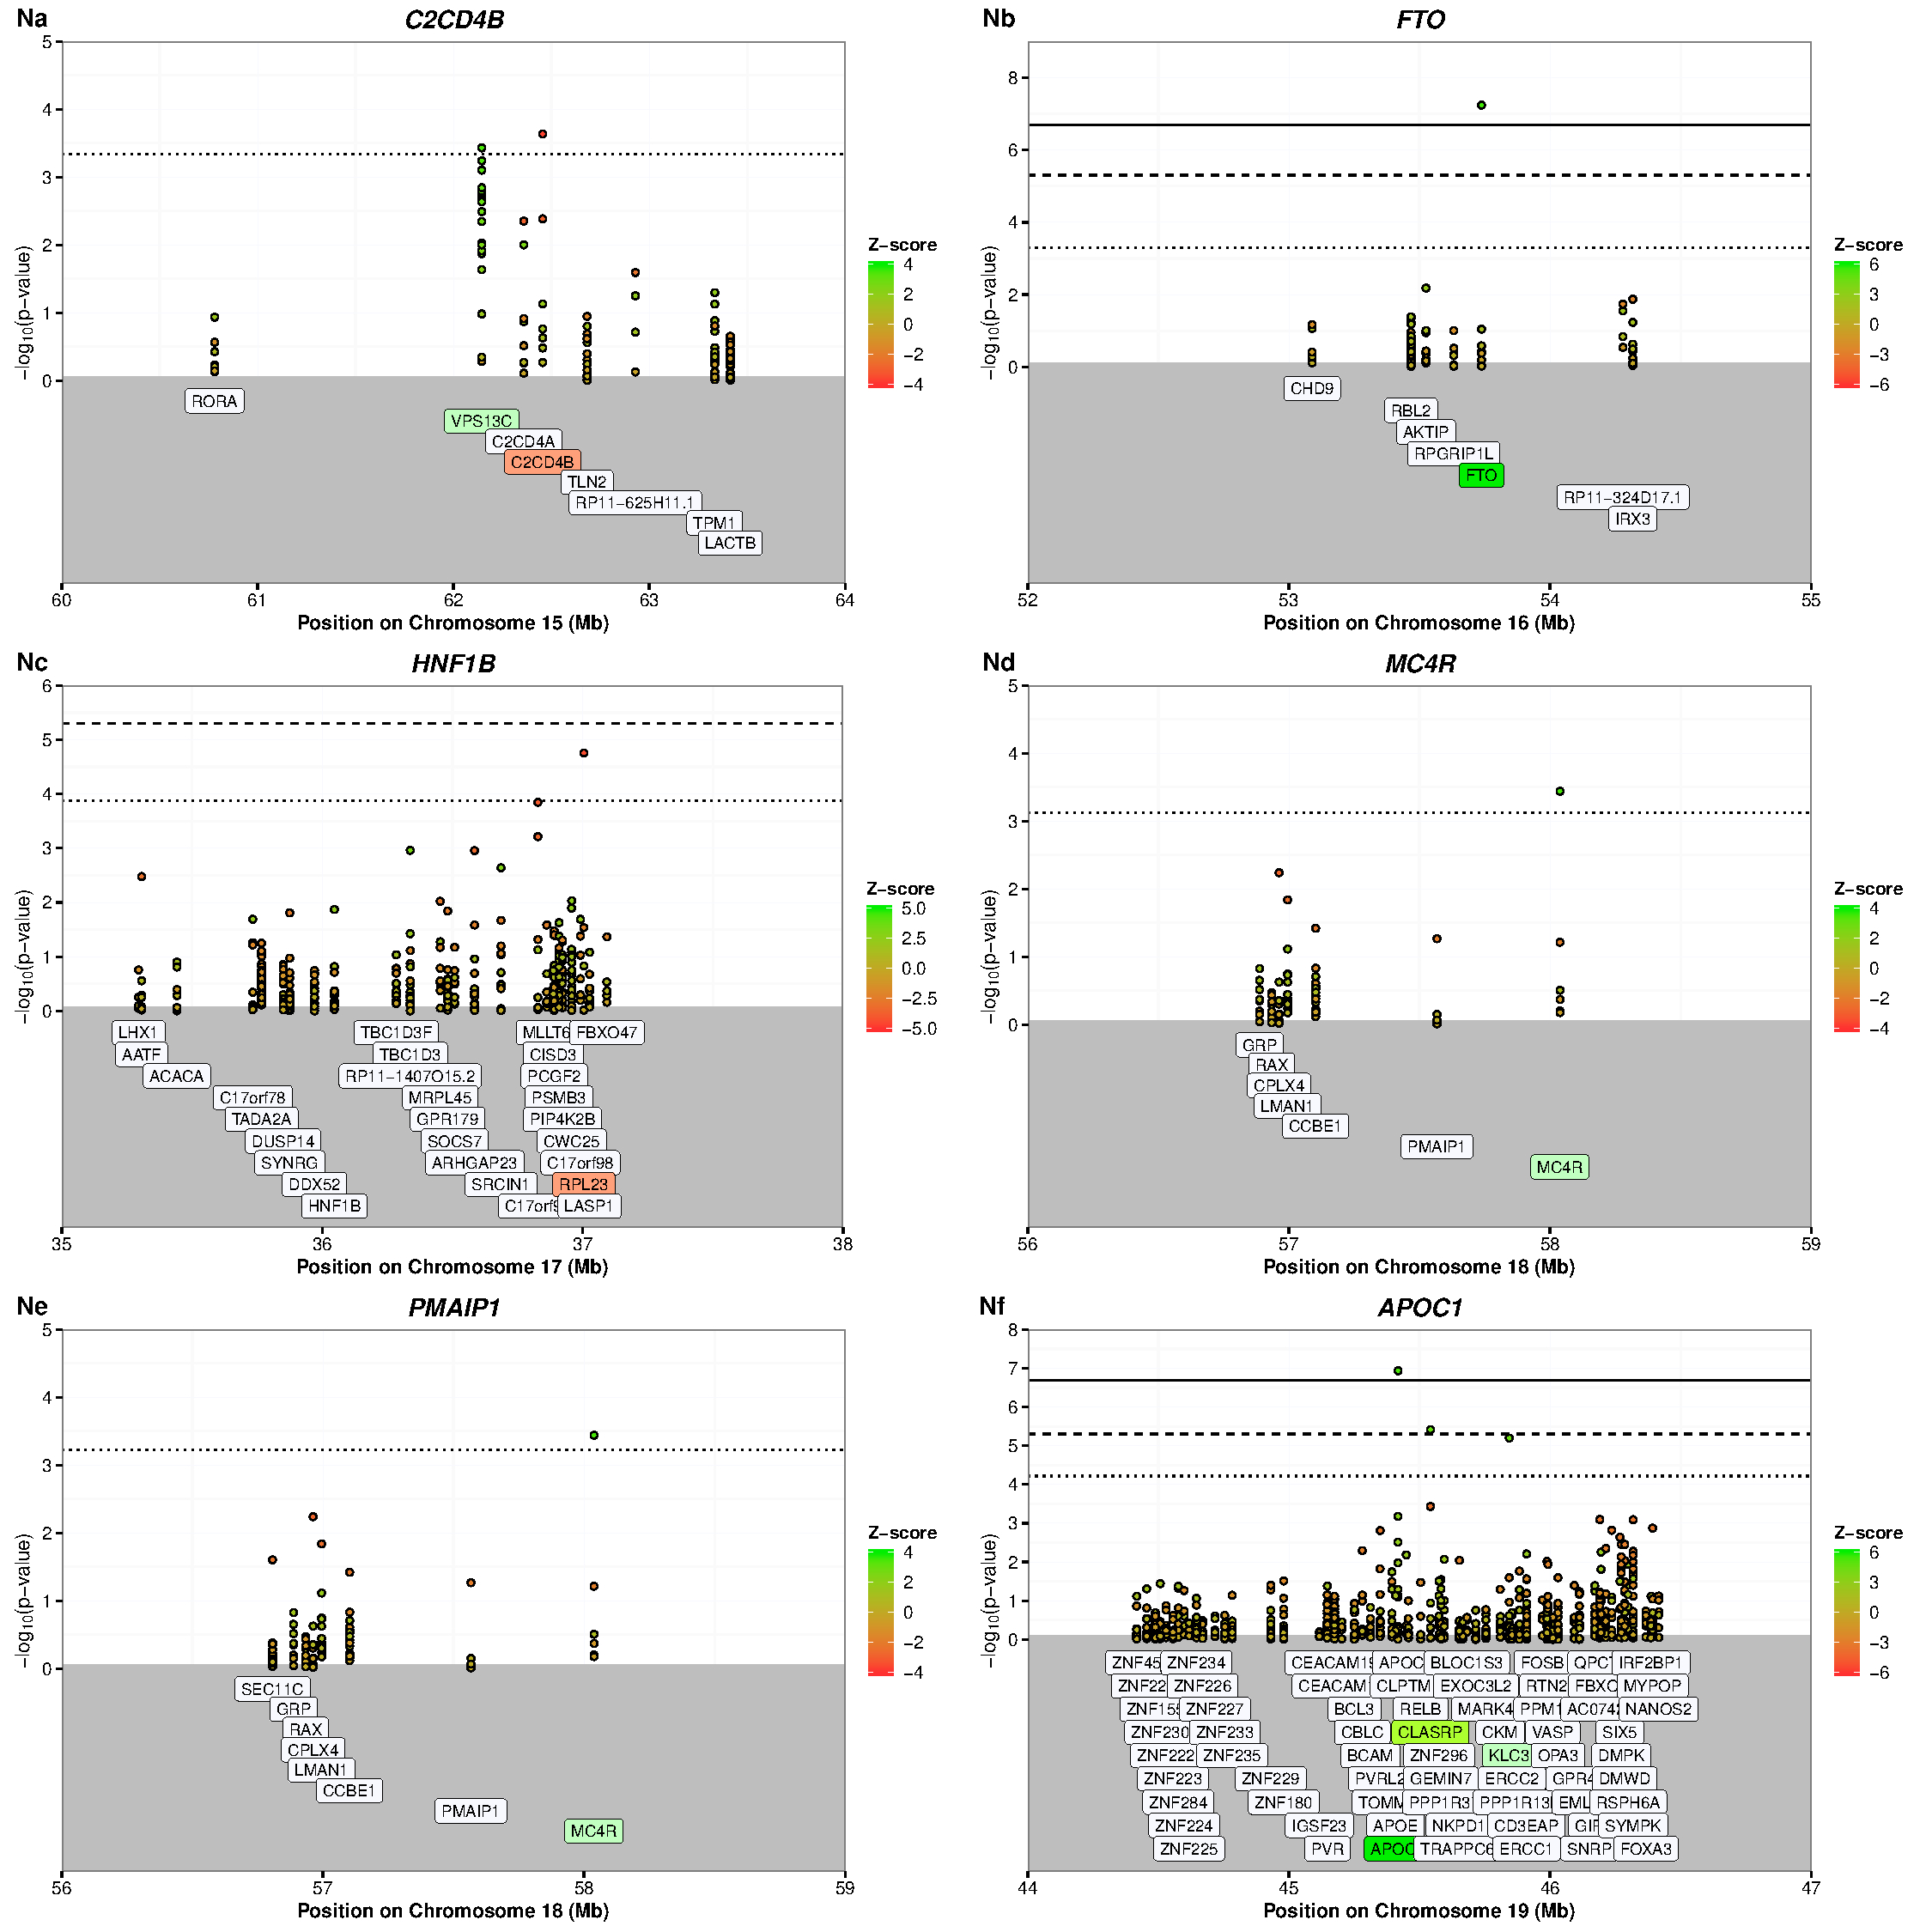
\includegraphics[width=\textwidth]{sup_fig1_part14_locusArray.pdf}
	\caption{\textbf{MetaXcan profiles at T2D-associated loci} We tested for association between predicted gene expression and T2D at $\sim2$ Mb genomic regions encompassing putative T2D genes implicated by the top $1,000$ SNPs associated with T2D from the DIAGRAM trans-ethnic meta-analysis of GWASs using $42$ tissue-level prediction models. The gene about which the genomic region is centered is indicated at the top of each panel. The solid, dashed, and dotted line denote significance correcting for the total number of tests performed across all models, genome-wide significance in a single model ($10,000$ tests), and locus-wide significance, respectively. Genomic position (Mb) and significance ($-\log_{10}$(p-value)) for each predicted gene expression value (from a particular tissue model) are shown on the $x$ and $y$-axis, respectively. Gene labels are shown in the gray region and are positioned at the transcription start site (TSS). Moreover, color corresponds to the magnitude and sign of the $Z$-score where positive and negative $Z$-scores are colored green and red, respectively.} 
    \label{fig:supp.locus_array_fig1_part14}
\end{figure}

\begin{figure}
\ContinuedFloat
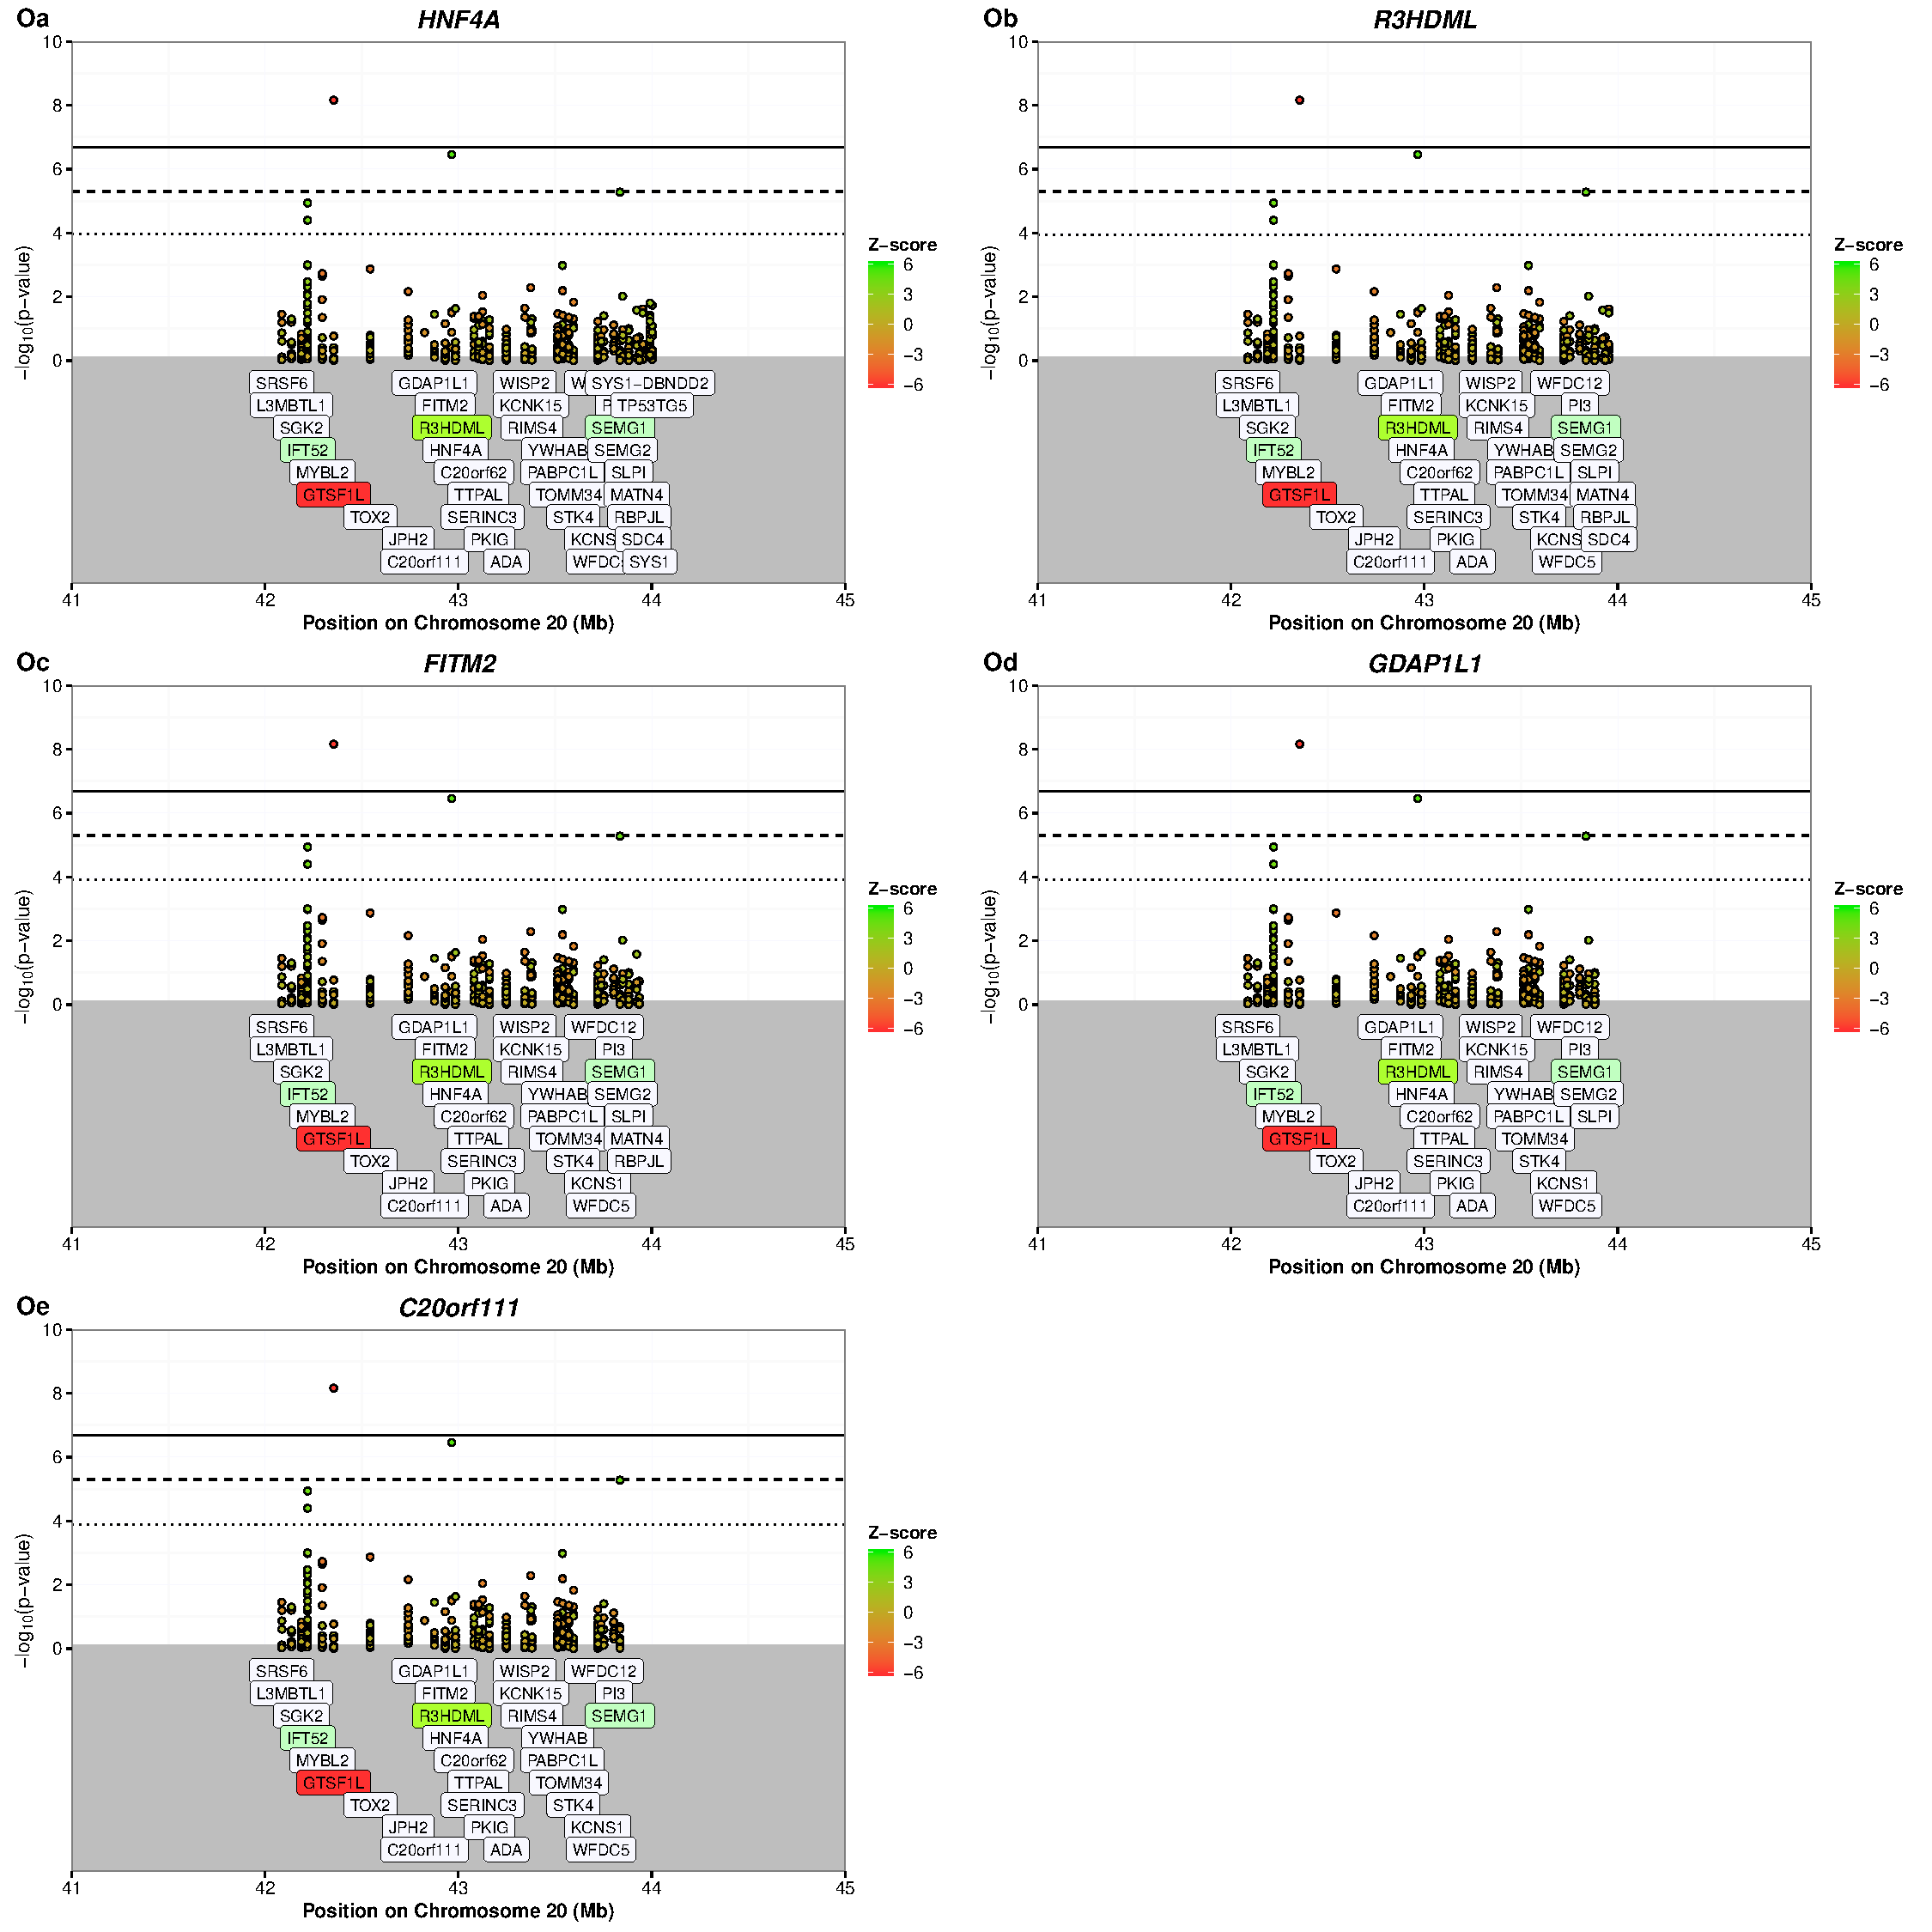
\includegraphics[width=\textwidth]{sup_fig1_part15_locusArray.pdf}
	\caption{\textbf{MetaXcan profiles at T2D-associated loci} We tested for association between predicted gene expression and T2D at $\sim2$ Mb genomic regions encompassing putative T2D genes implicated by the top $1,000$ SNPs associated with T2D from the DIAGRAM trans-ethnic meta-analysis of GWASs using $42$ tissue-level prediction models. The gene about which the genomic region is centered is indicated at the top of each panel. The solid, dashed, and dotted line denote significance correcting for the total number of tests performed across all models, genome-wide significance in a single model ($10,000$ tests), and locus-wide significance, respectively. Genomic position (Mb) and significance ($-\log_{10}$(p-value)) for each predicted gene expression value (from a particular tissue model) are shown on the $x$ and $y$-axis, respectively. Gene labels are shown in the gray region and are positioned at the transcription start site (TSS). Moreover, color corresponds to the magnitude and sign of the $Z$-score where positive and negative $Z$-scores are colored green and red, respectively.} 
    \label{fig:supp.locus_array_fig1_part15}
\end{figure}

% Supplementary Figure 2

\begin{figure}
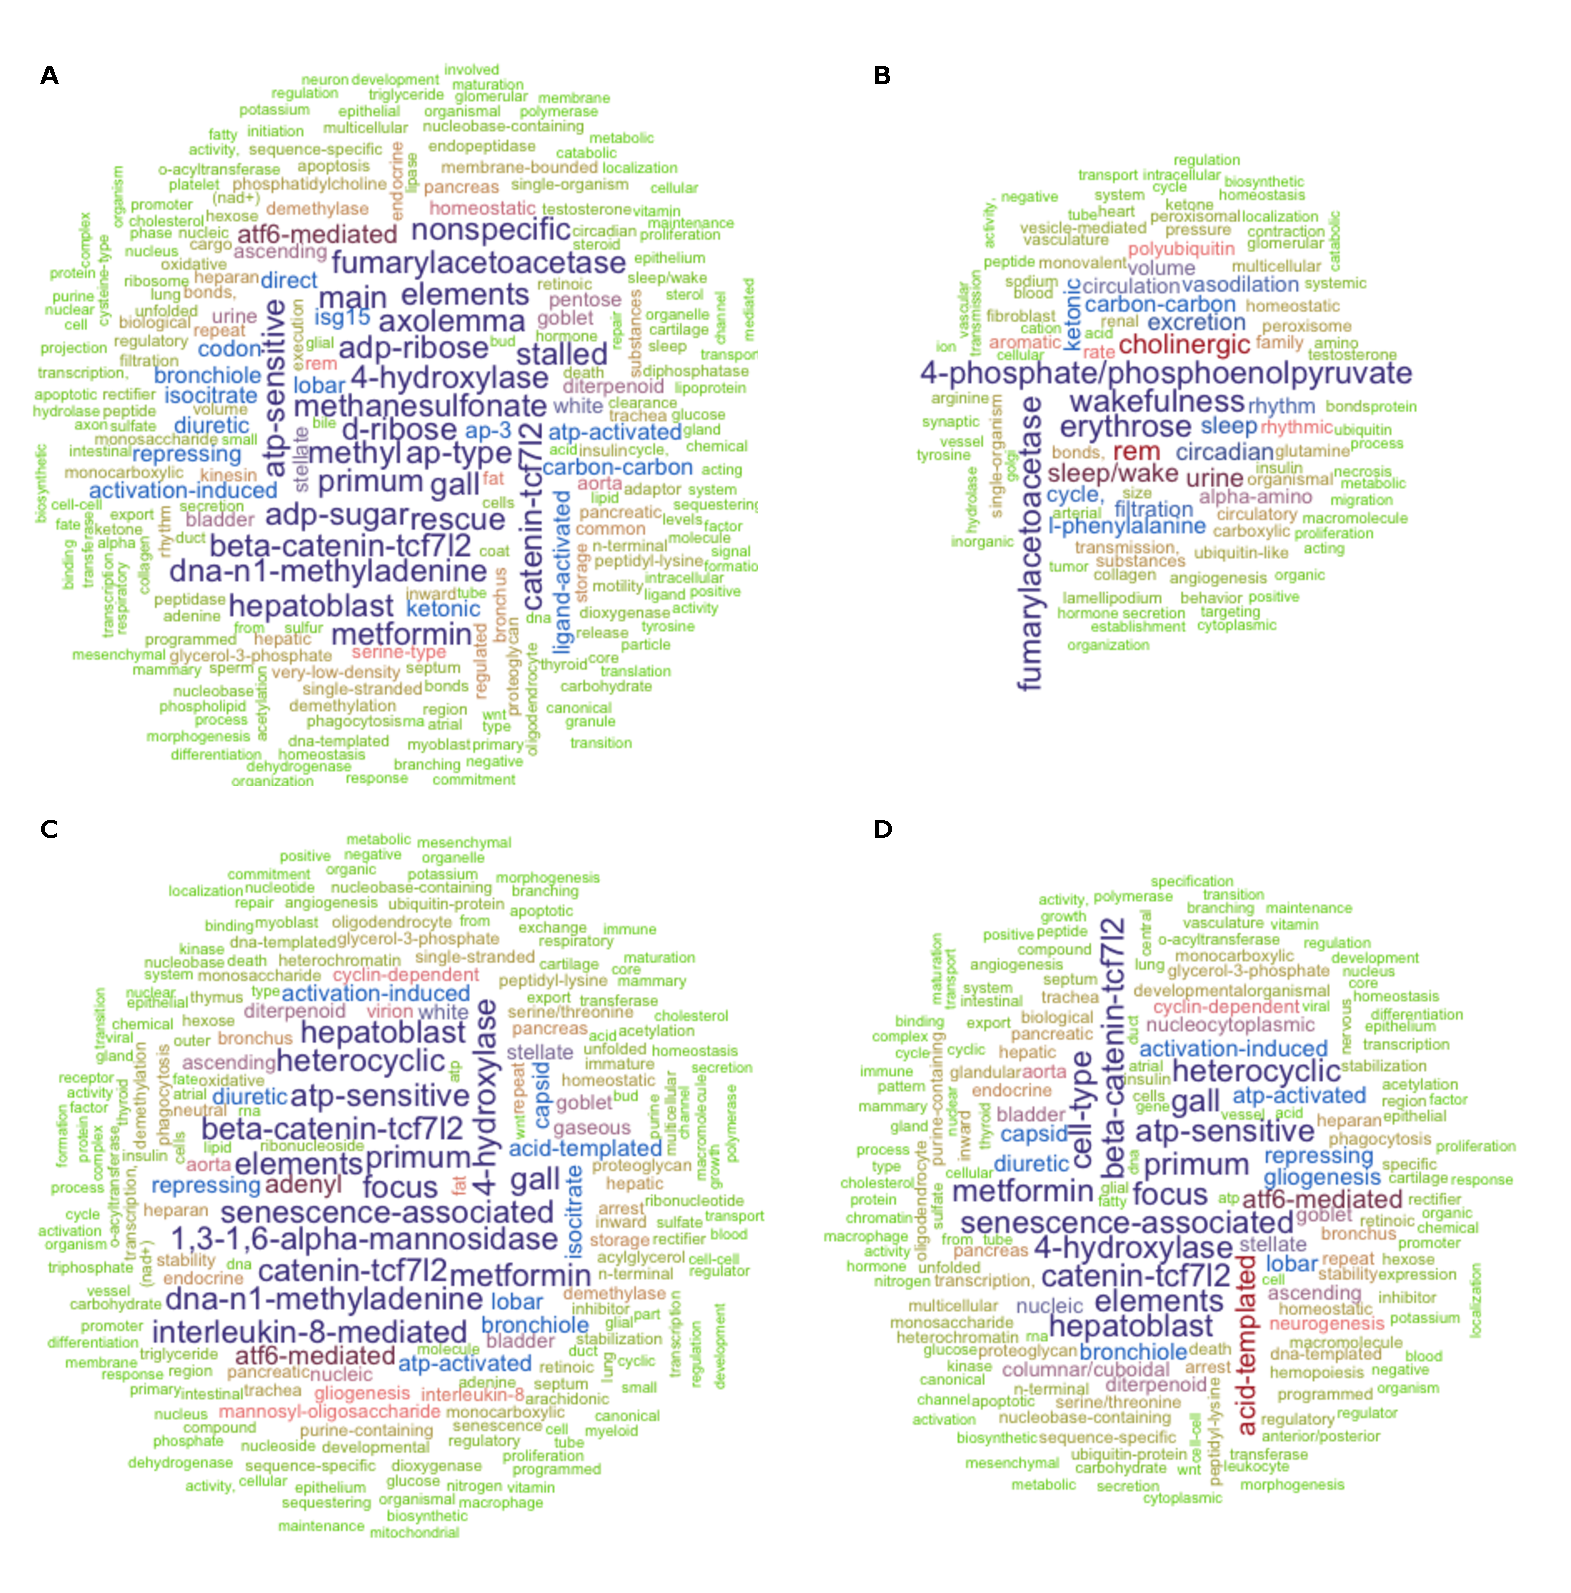
\includegraphics[width=\textwidth]{wordplots.pdf}
	\caption{\textbf{Text-mining analysis of frequently occurring terms among enriched pathways from MetaXcan-significant gene sets.} We text-mined the set of Gene Ontology Biological Process (GO:BP) pathways that were enriched (overrepresented p-value $\leq 0.05$) among sets of genes meeting genome-wide significance in at least on tissue from our MetaXcan analyses. Wordlcouds show the most frequently occurring terms (larger font and centrally located) - limited to no more than the top $200$ terms. Results are shown for: (A) all genes meeting genome-wide significance in at least one tissue from the DIAGRAM analyses; (B) the subset of genes in A that are not located within $1$ Mb of T2D-associated SNPs; (C) genome-wide significant genes from the meta-analysis of MetaXcan results from the DIAGRAM and GERA analyses; (D) all genes meeting genome-wide significance in at least one tissue discovered in the DIAGRAM analysis that replicate in the GERA analysis.} 
    \label{fig:supp_fig2_wordplots}
\end{figure}


% Supplementary Table 1 (FDR < 5%) 
\begin{table}
	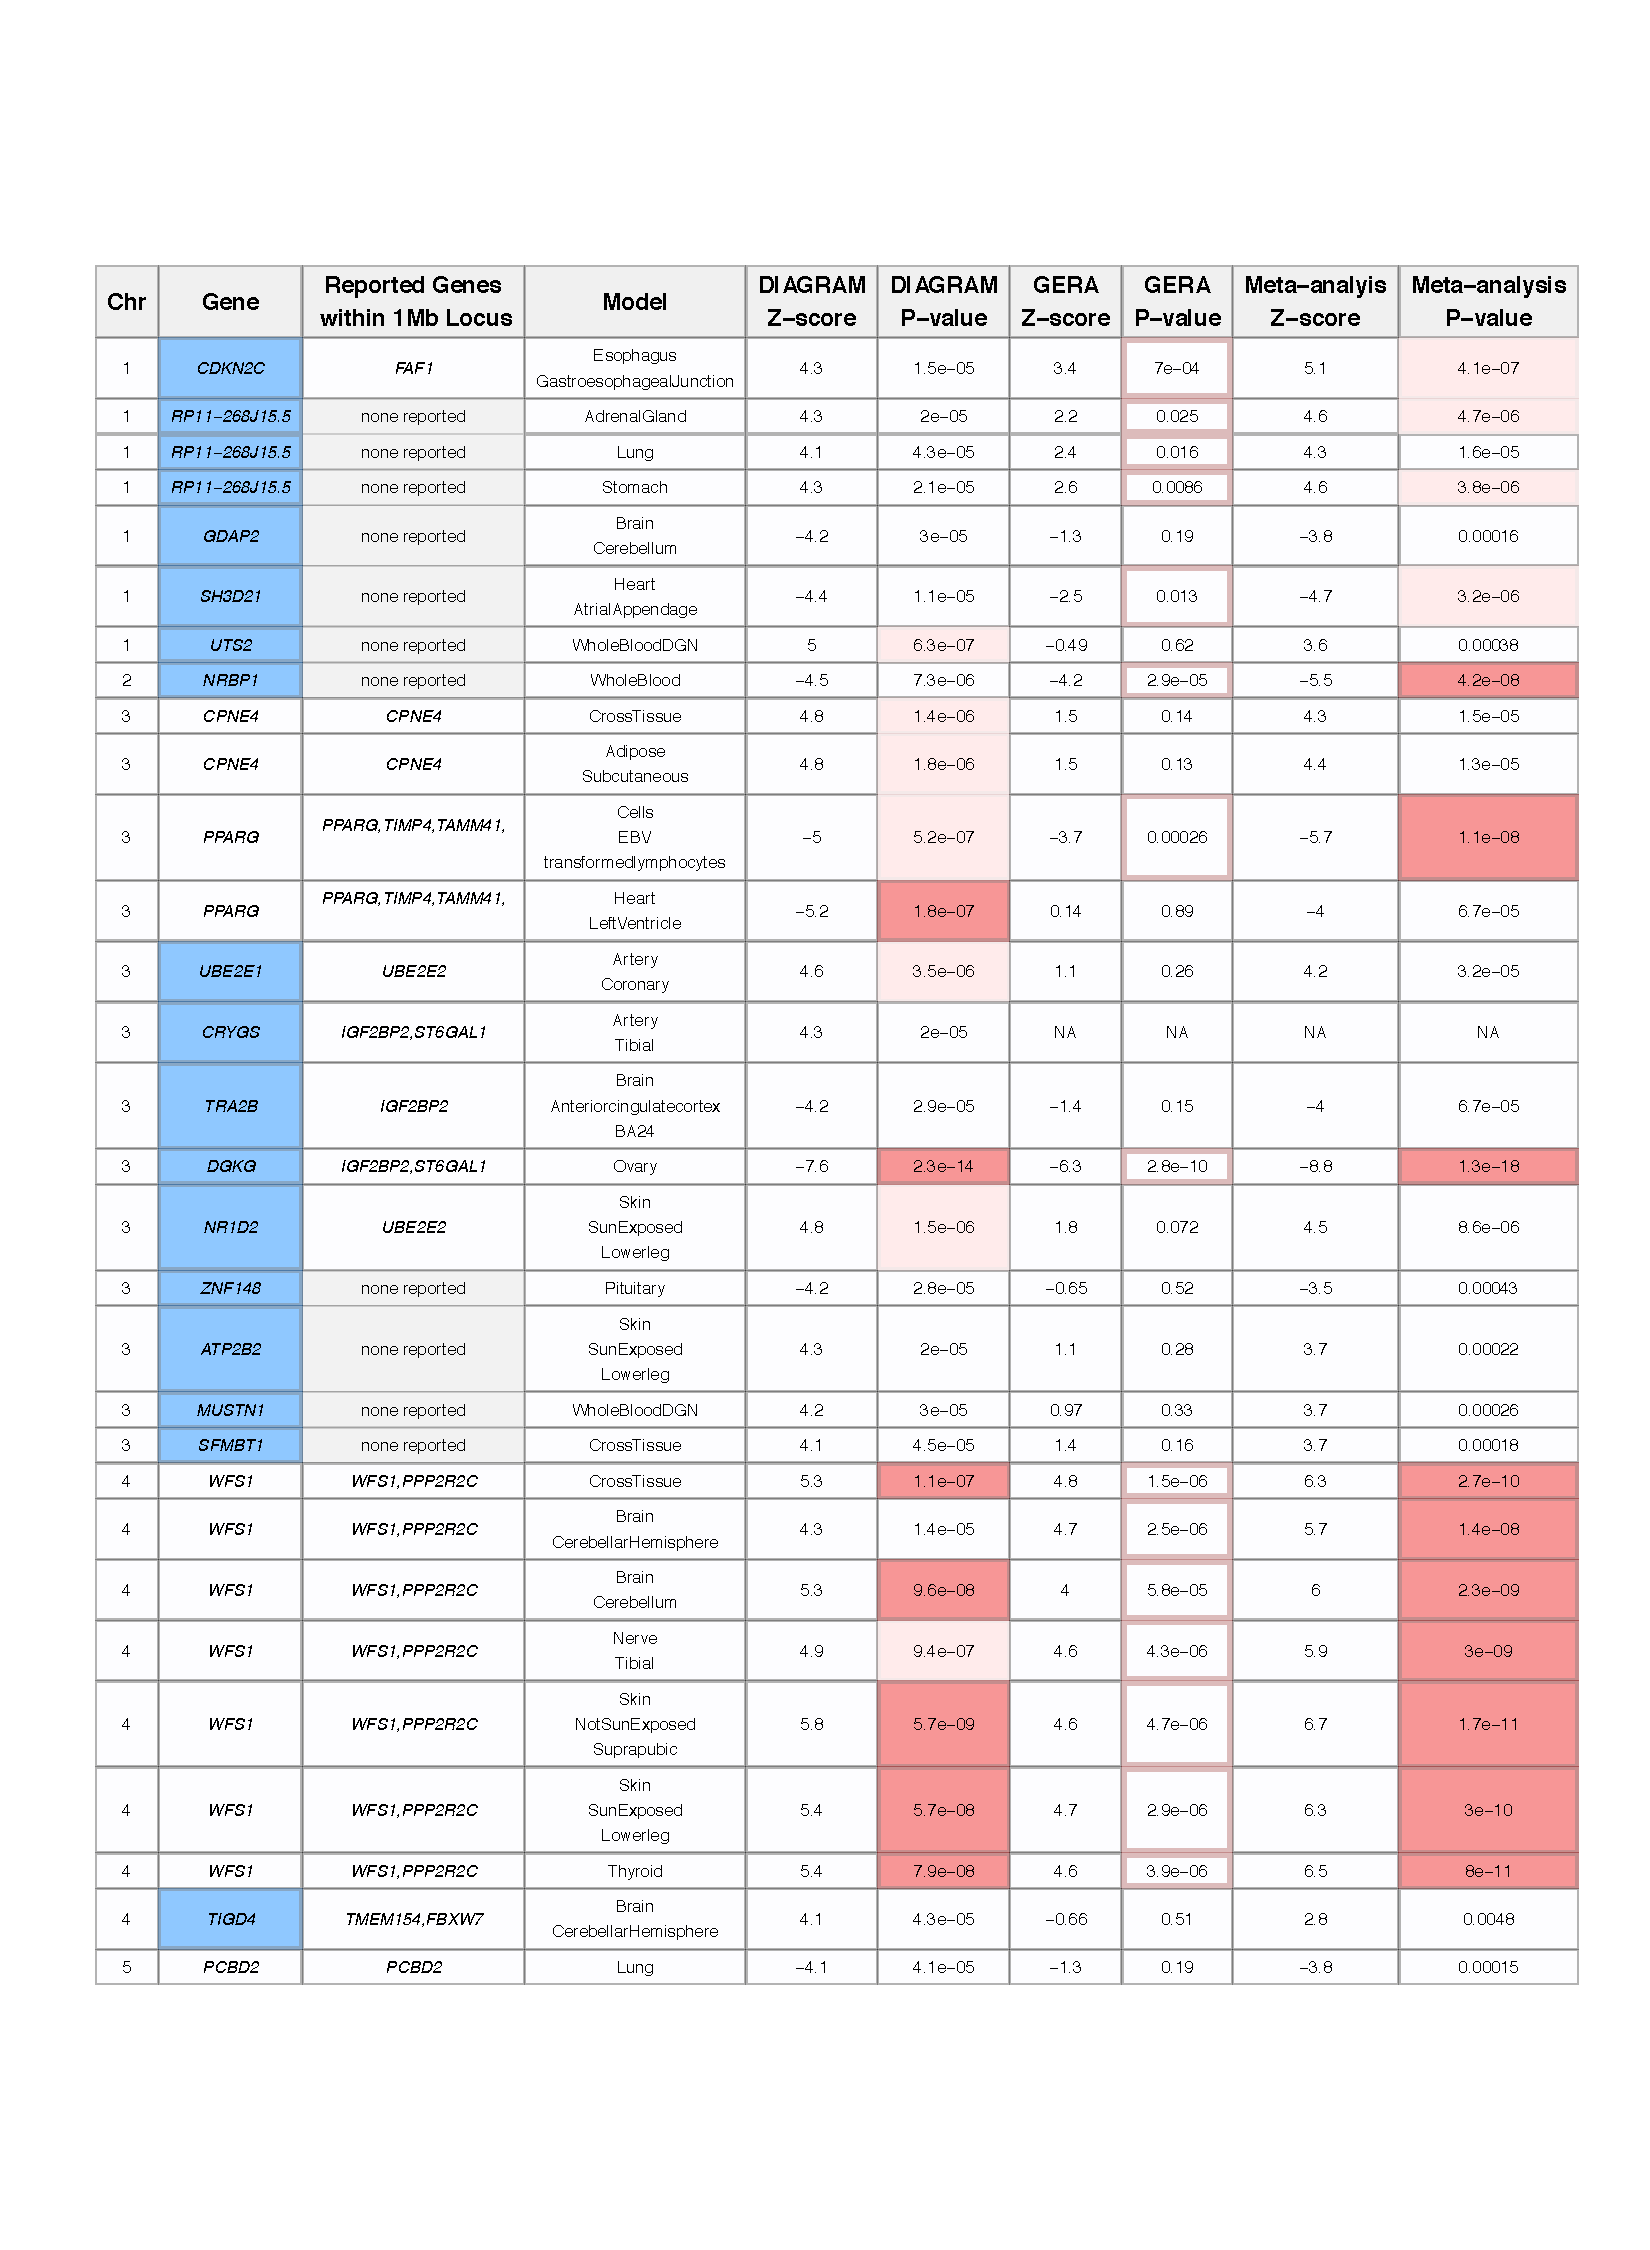
\includegraphics[width=0.95\textwidth]{supp_tab1_part1.pdf}
	\caption{\textbf{MetaXcan associations with T2D.} Results for genes and corresponding models that meet genome-wide significance \textit{in at least one model} from the DIAGRAM analysis are shown with nearby genes and results from the GERA replication study and meta-analysis of DIAGRAM and GERA Metaxcan associations. Blue shading denotes genes not implicated by the top $1,000$ SNPs from the DIAGRAM trans-ethnic meta-analysis of GWASs. Pink and red shading denote genome-wide significance in one model and across all models, respectively, for the DIAGRAM and meta-analysis. Replication in the GERA study is denoted by a pink outline.} 
	\label{tab:supp.table1.part1}
\end{table}

\begin{table}
	\ContinuedFloat
	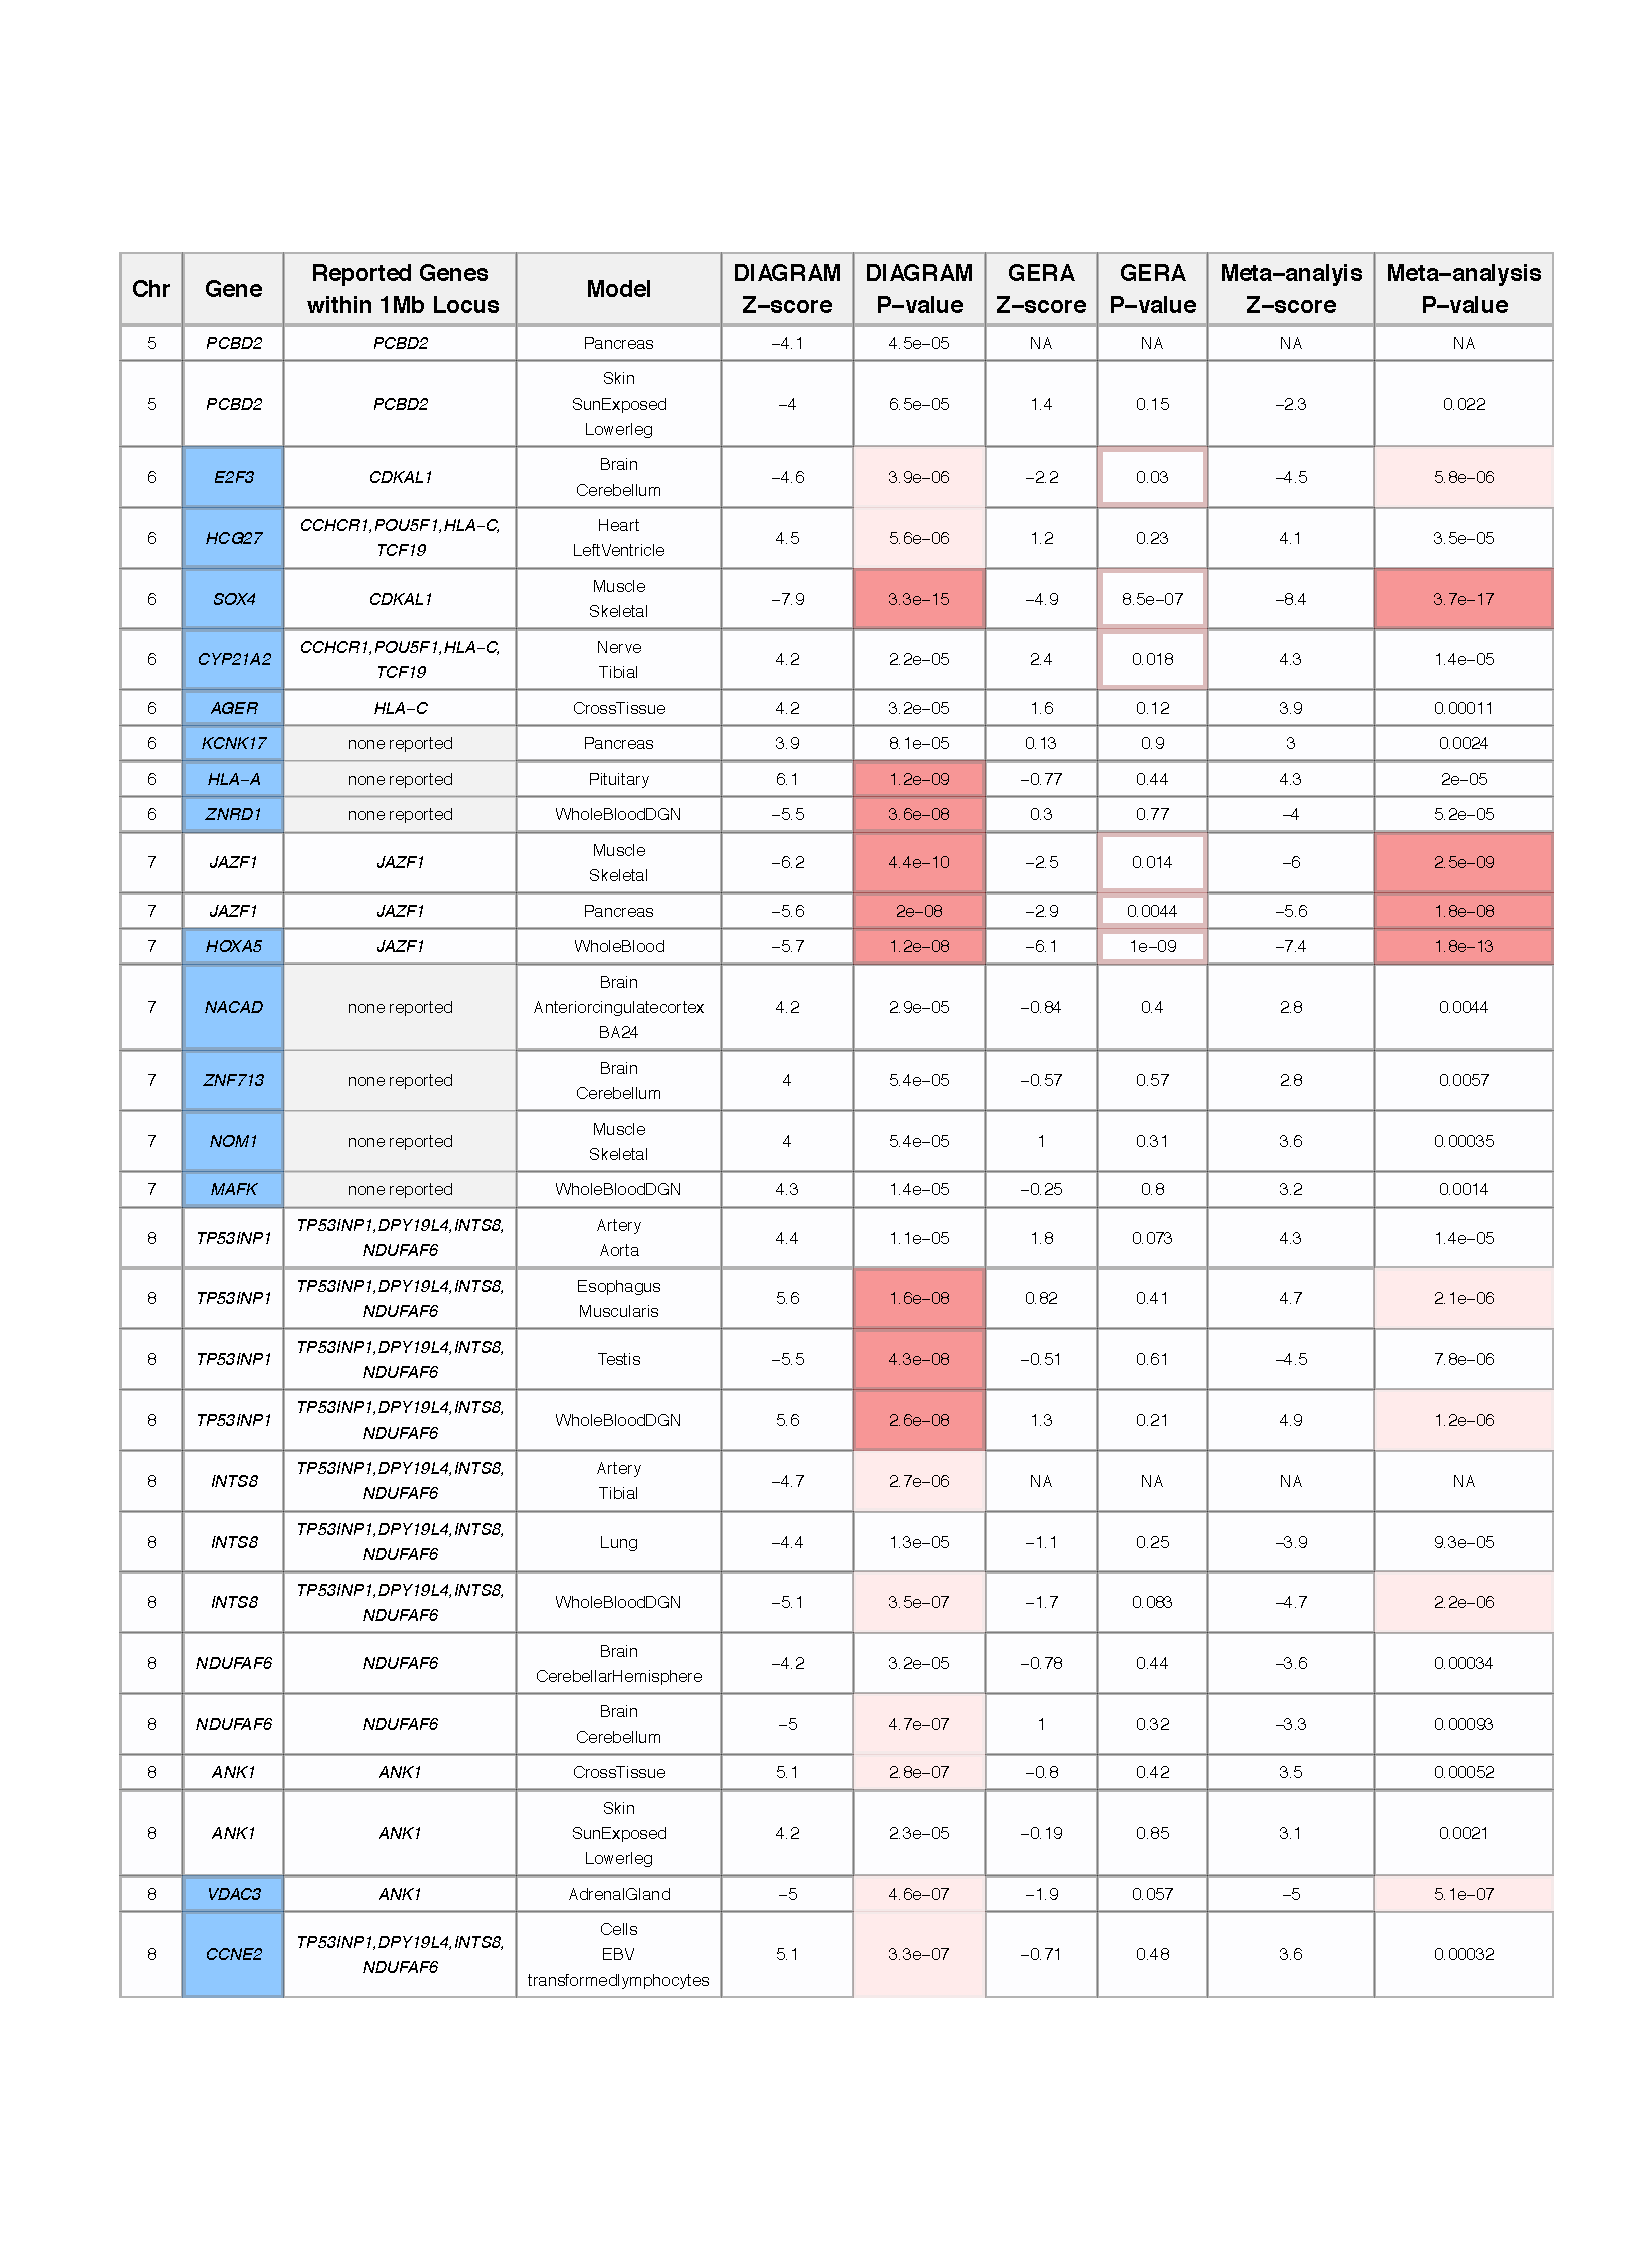
\includegraphics[width=0.9\textwidth]{supp_tab1_part2.pdf}
	\caption{\textbf{MetaXcan associations with T2D.} Results for genes and corresponding models that meet genome-wide significance \textit{in at least one model} from the DIAGRAM analysis are shown with nearby genes and results from the GERA replication study and meta-analysis of DIAGRAM and GERA Metaxcan associations. Blue shading denotes genes not implicated by the top $1,000$ SNPs from the DIAGRAM trans-ethnic meta-analysis of GWASs. Pink and red shading denote genome-wide significance in one model and across all models, respectively, for the DIAGRAM and meta-analysis. Replication in the GERA study is denoted by a pink outline.} 
	\label{tab:supp.table1.part2}
\end{table}

\clearpage
\begin{table}
	\ContinuedFloat
	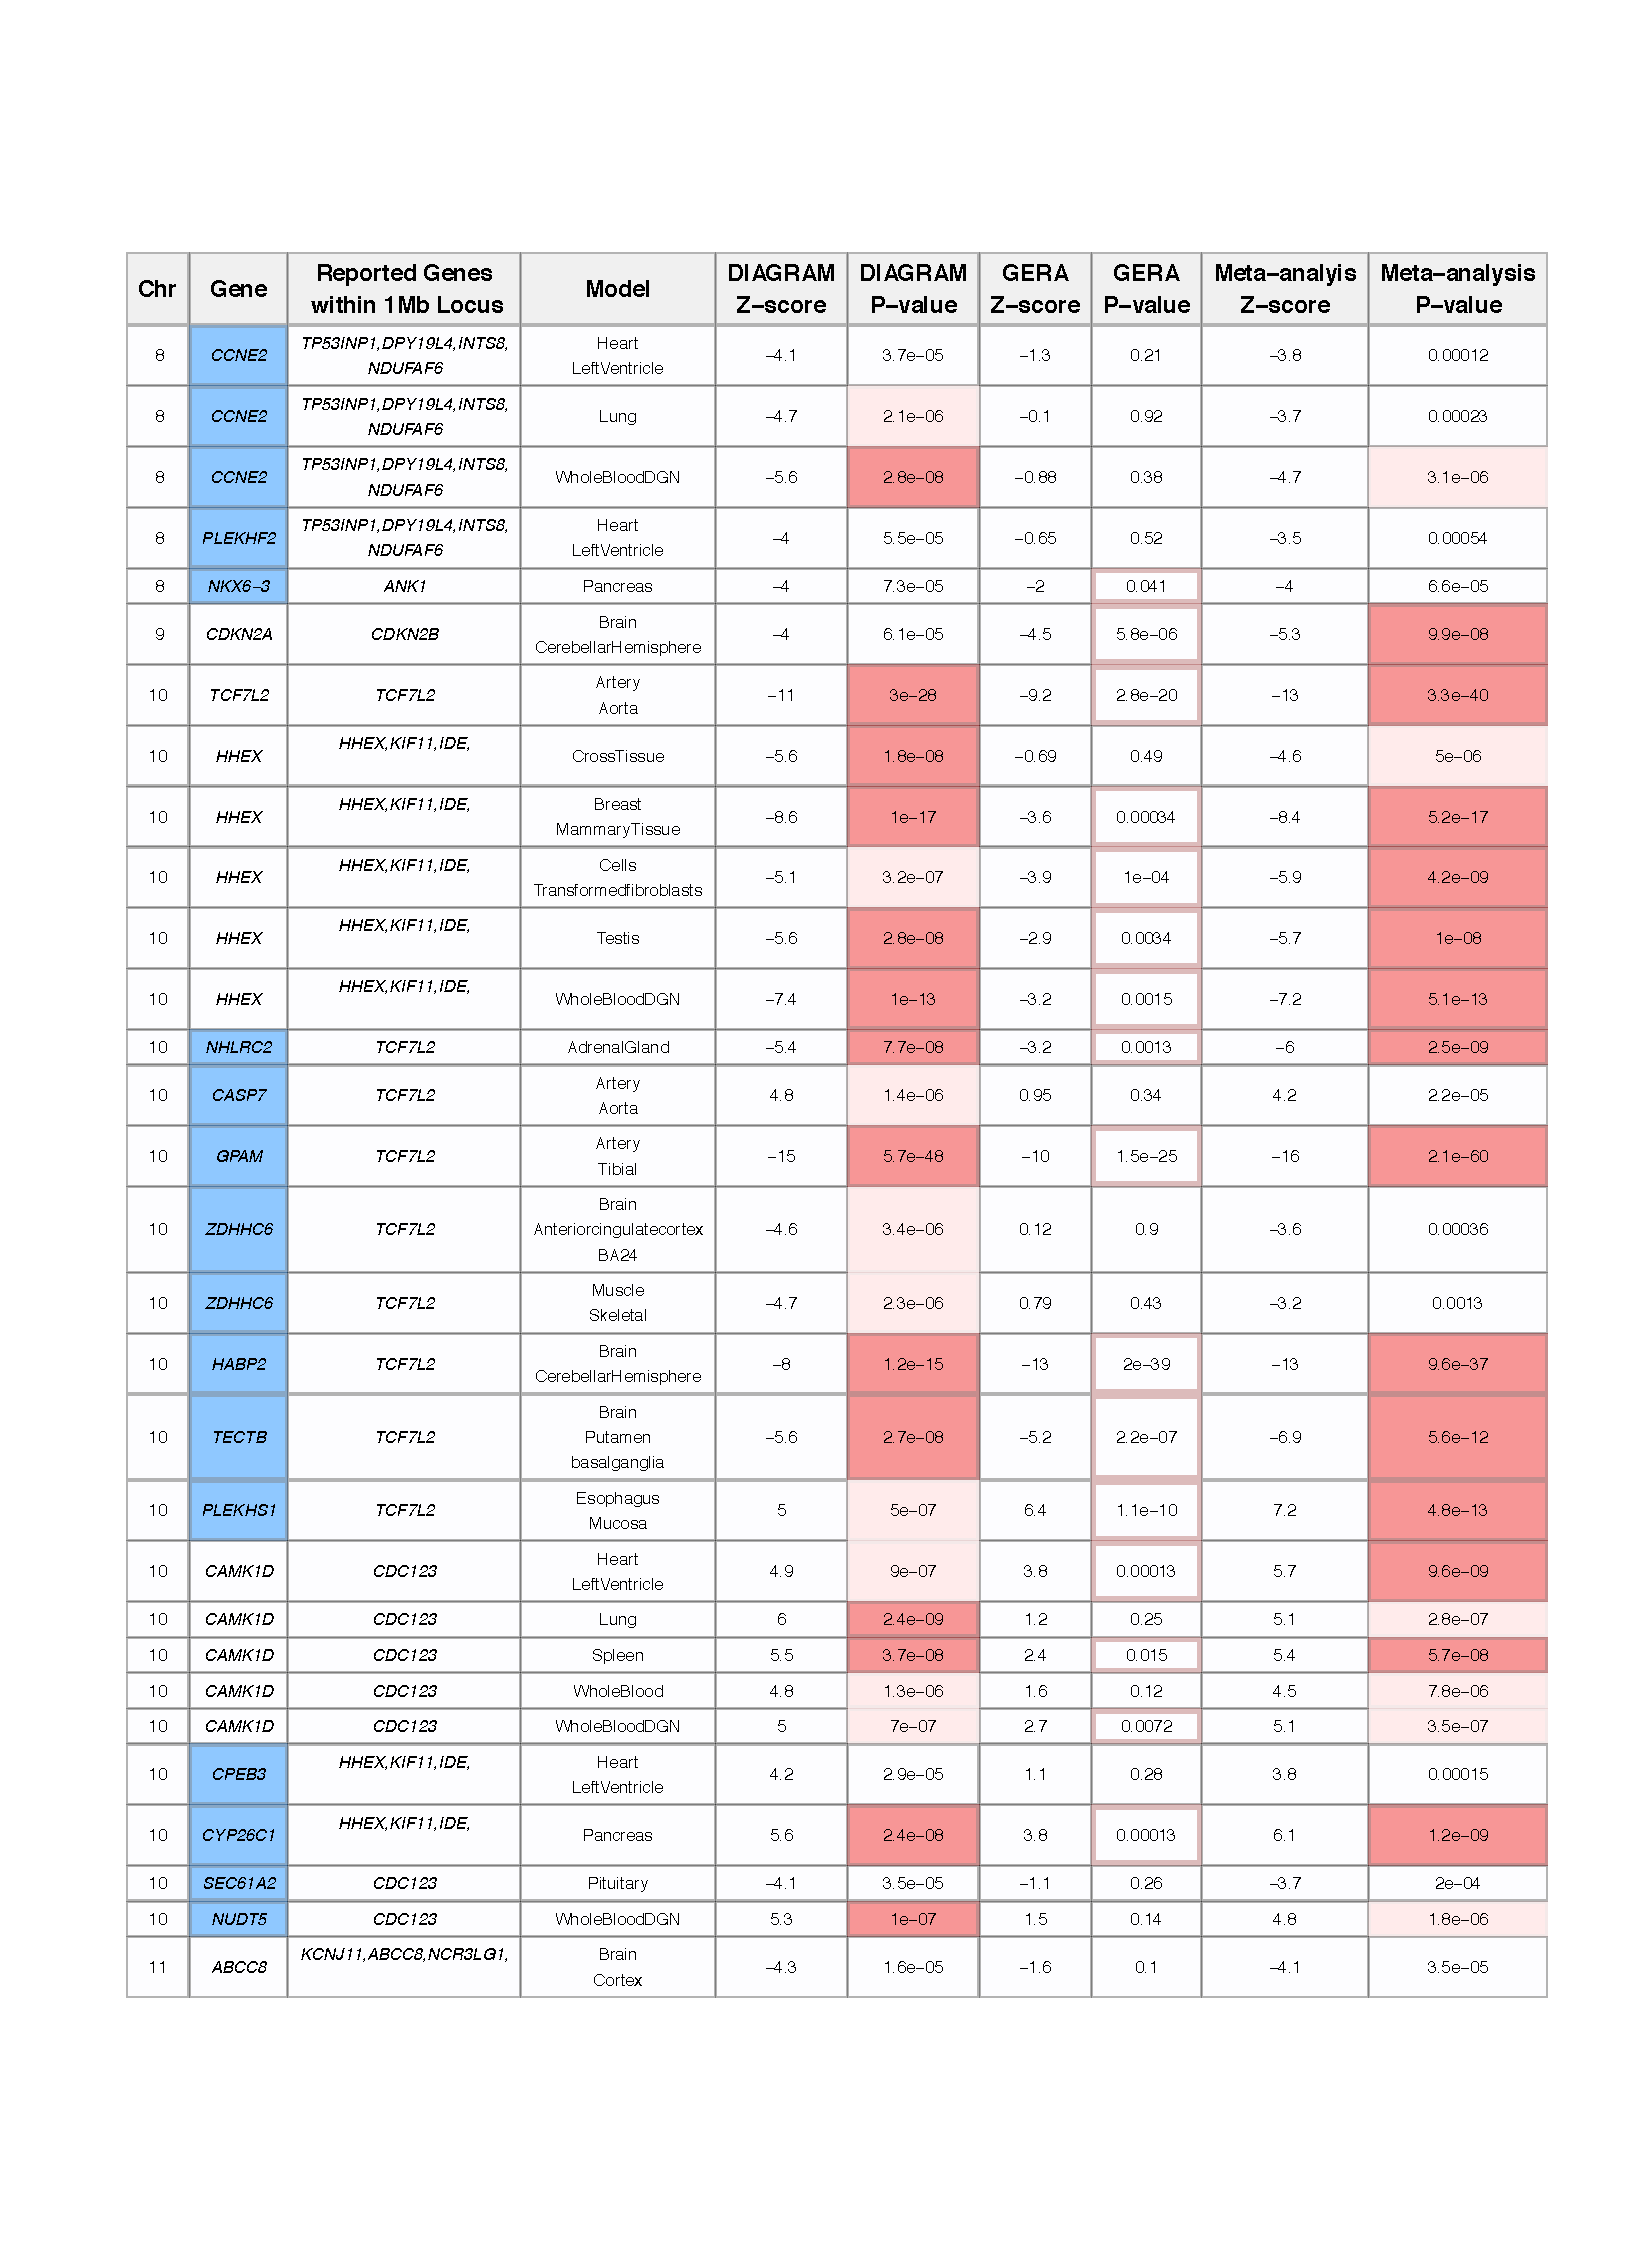
\includegraphics[width=0.90\textwidth]{supp_tab1_part3.pdf}
	\caption{\textbf{MetaXcan associations with T2D.} Results for genes and corresponding models that meet genome-wide significance \textit{in at least one model} from the DIAGRAM analysis are shown with nearby genes and results from the GERA replication study and meta-analysis of DIAGRAM and GERA Metaxcan associations. Blue shading denotes genes not implicated by the top $1,000$ SNPs from the DIAGRAM trans-ethnic meta-analysis of GWASs. Pink and red shading denote genome-wide significance in one model and across all models, respectively, for the DIAGRAM and meta-analysis. Replication in the GERA study is denoted by a pink outline.} 
	\label{tab:supp.table1.part3}
\end{table}

\clearpage
\begin{table}
\ContinuedFloat
	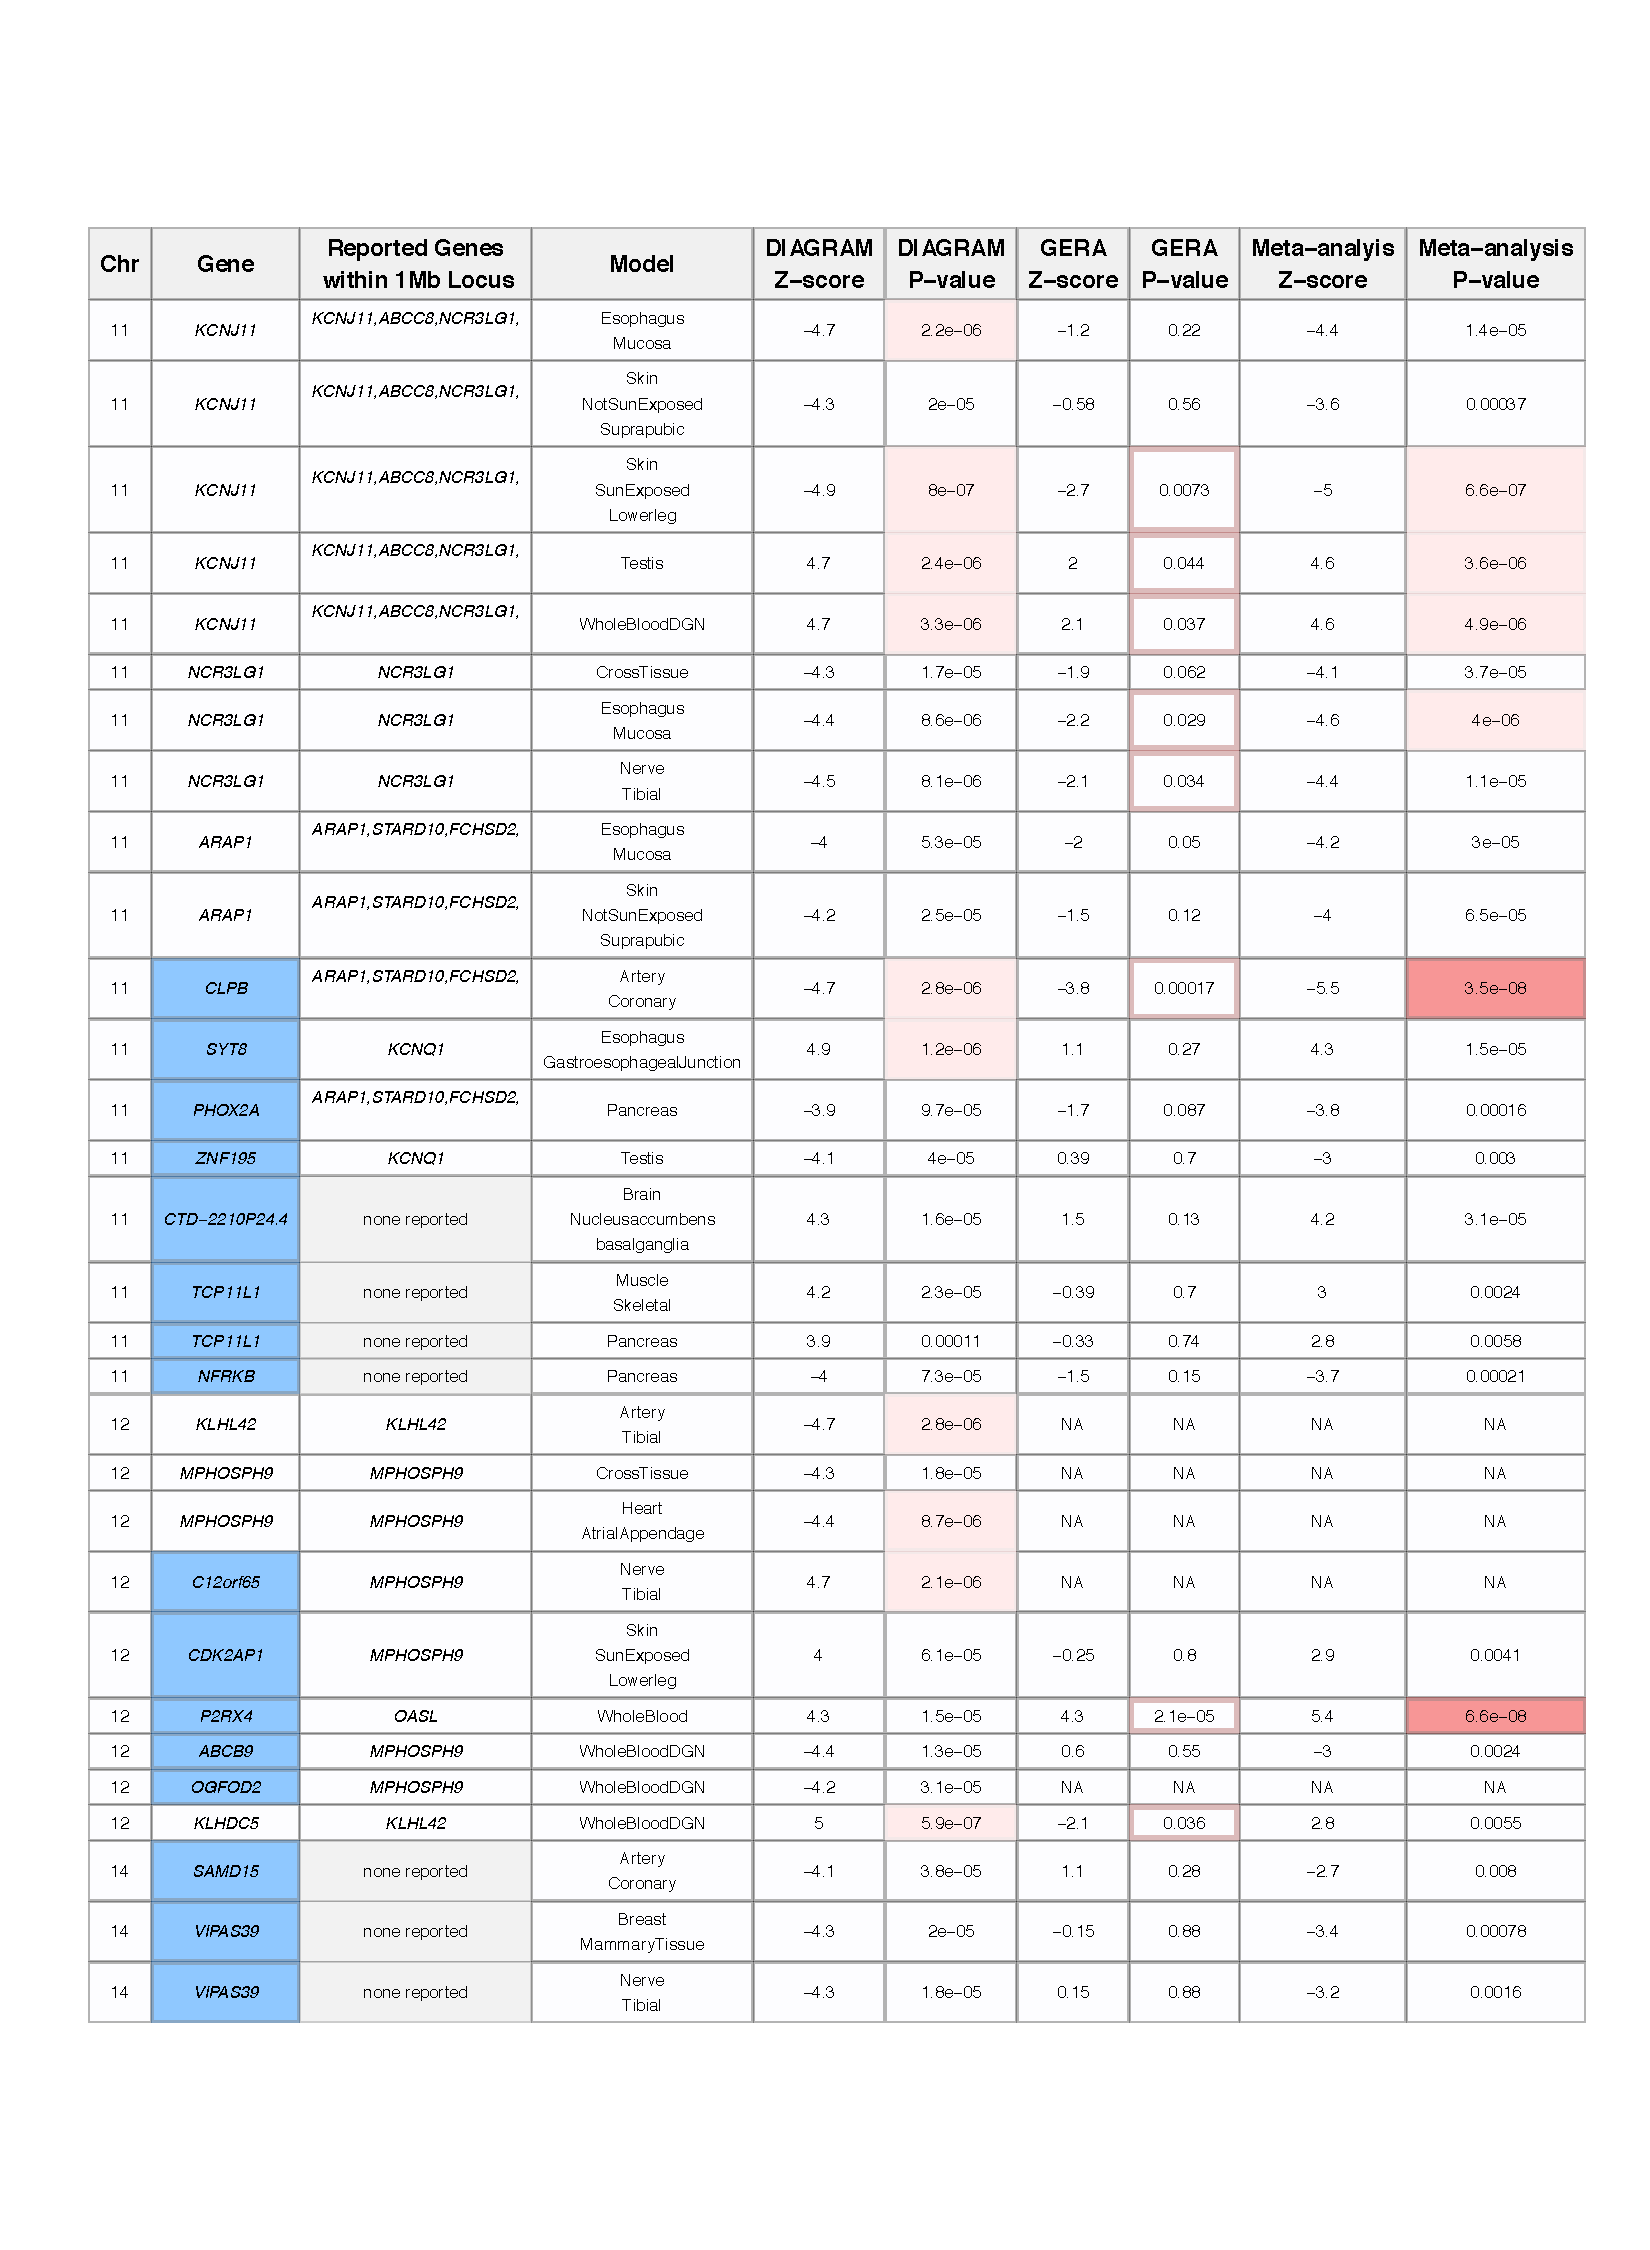
\includegraphics[width=0.90\textwidth]{supp_tab1_part4.pdf}
	\caption{\textbf{MetaXcan associations with T2D.} Results for genes and corresponding models that meet genome-wide significance \textit{in at least one model} from the DIAGRAM analysis are shown with nearby genes and results from the GERA replication study and meta-analysis of DIAGRAM and GERA Metaxcan associations. Blue shading denotes genes not implicated by the top $1,000$ SNPs from the DIAGRAM trans-ethnic meta-analysis of GWASs. Pink and red shading denote genome-wide significance in one model and across all models, respectively, for the DIAGRAM and meta-analysis. Replication in the GERA study is denoted by a pink outline.} 
	\label{tab:supp.table1.part4}
\end{table}

\begin{table}
\ContinuedFloat
	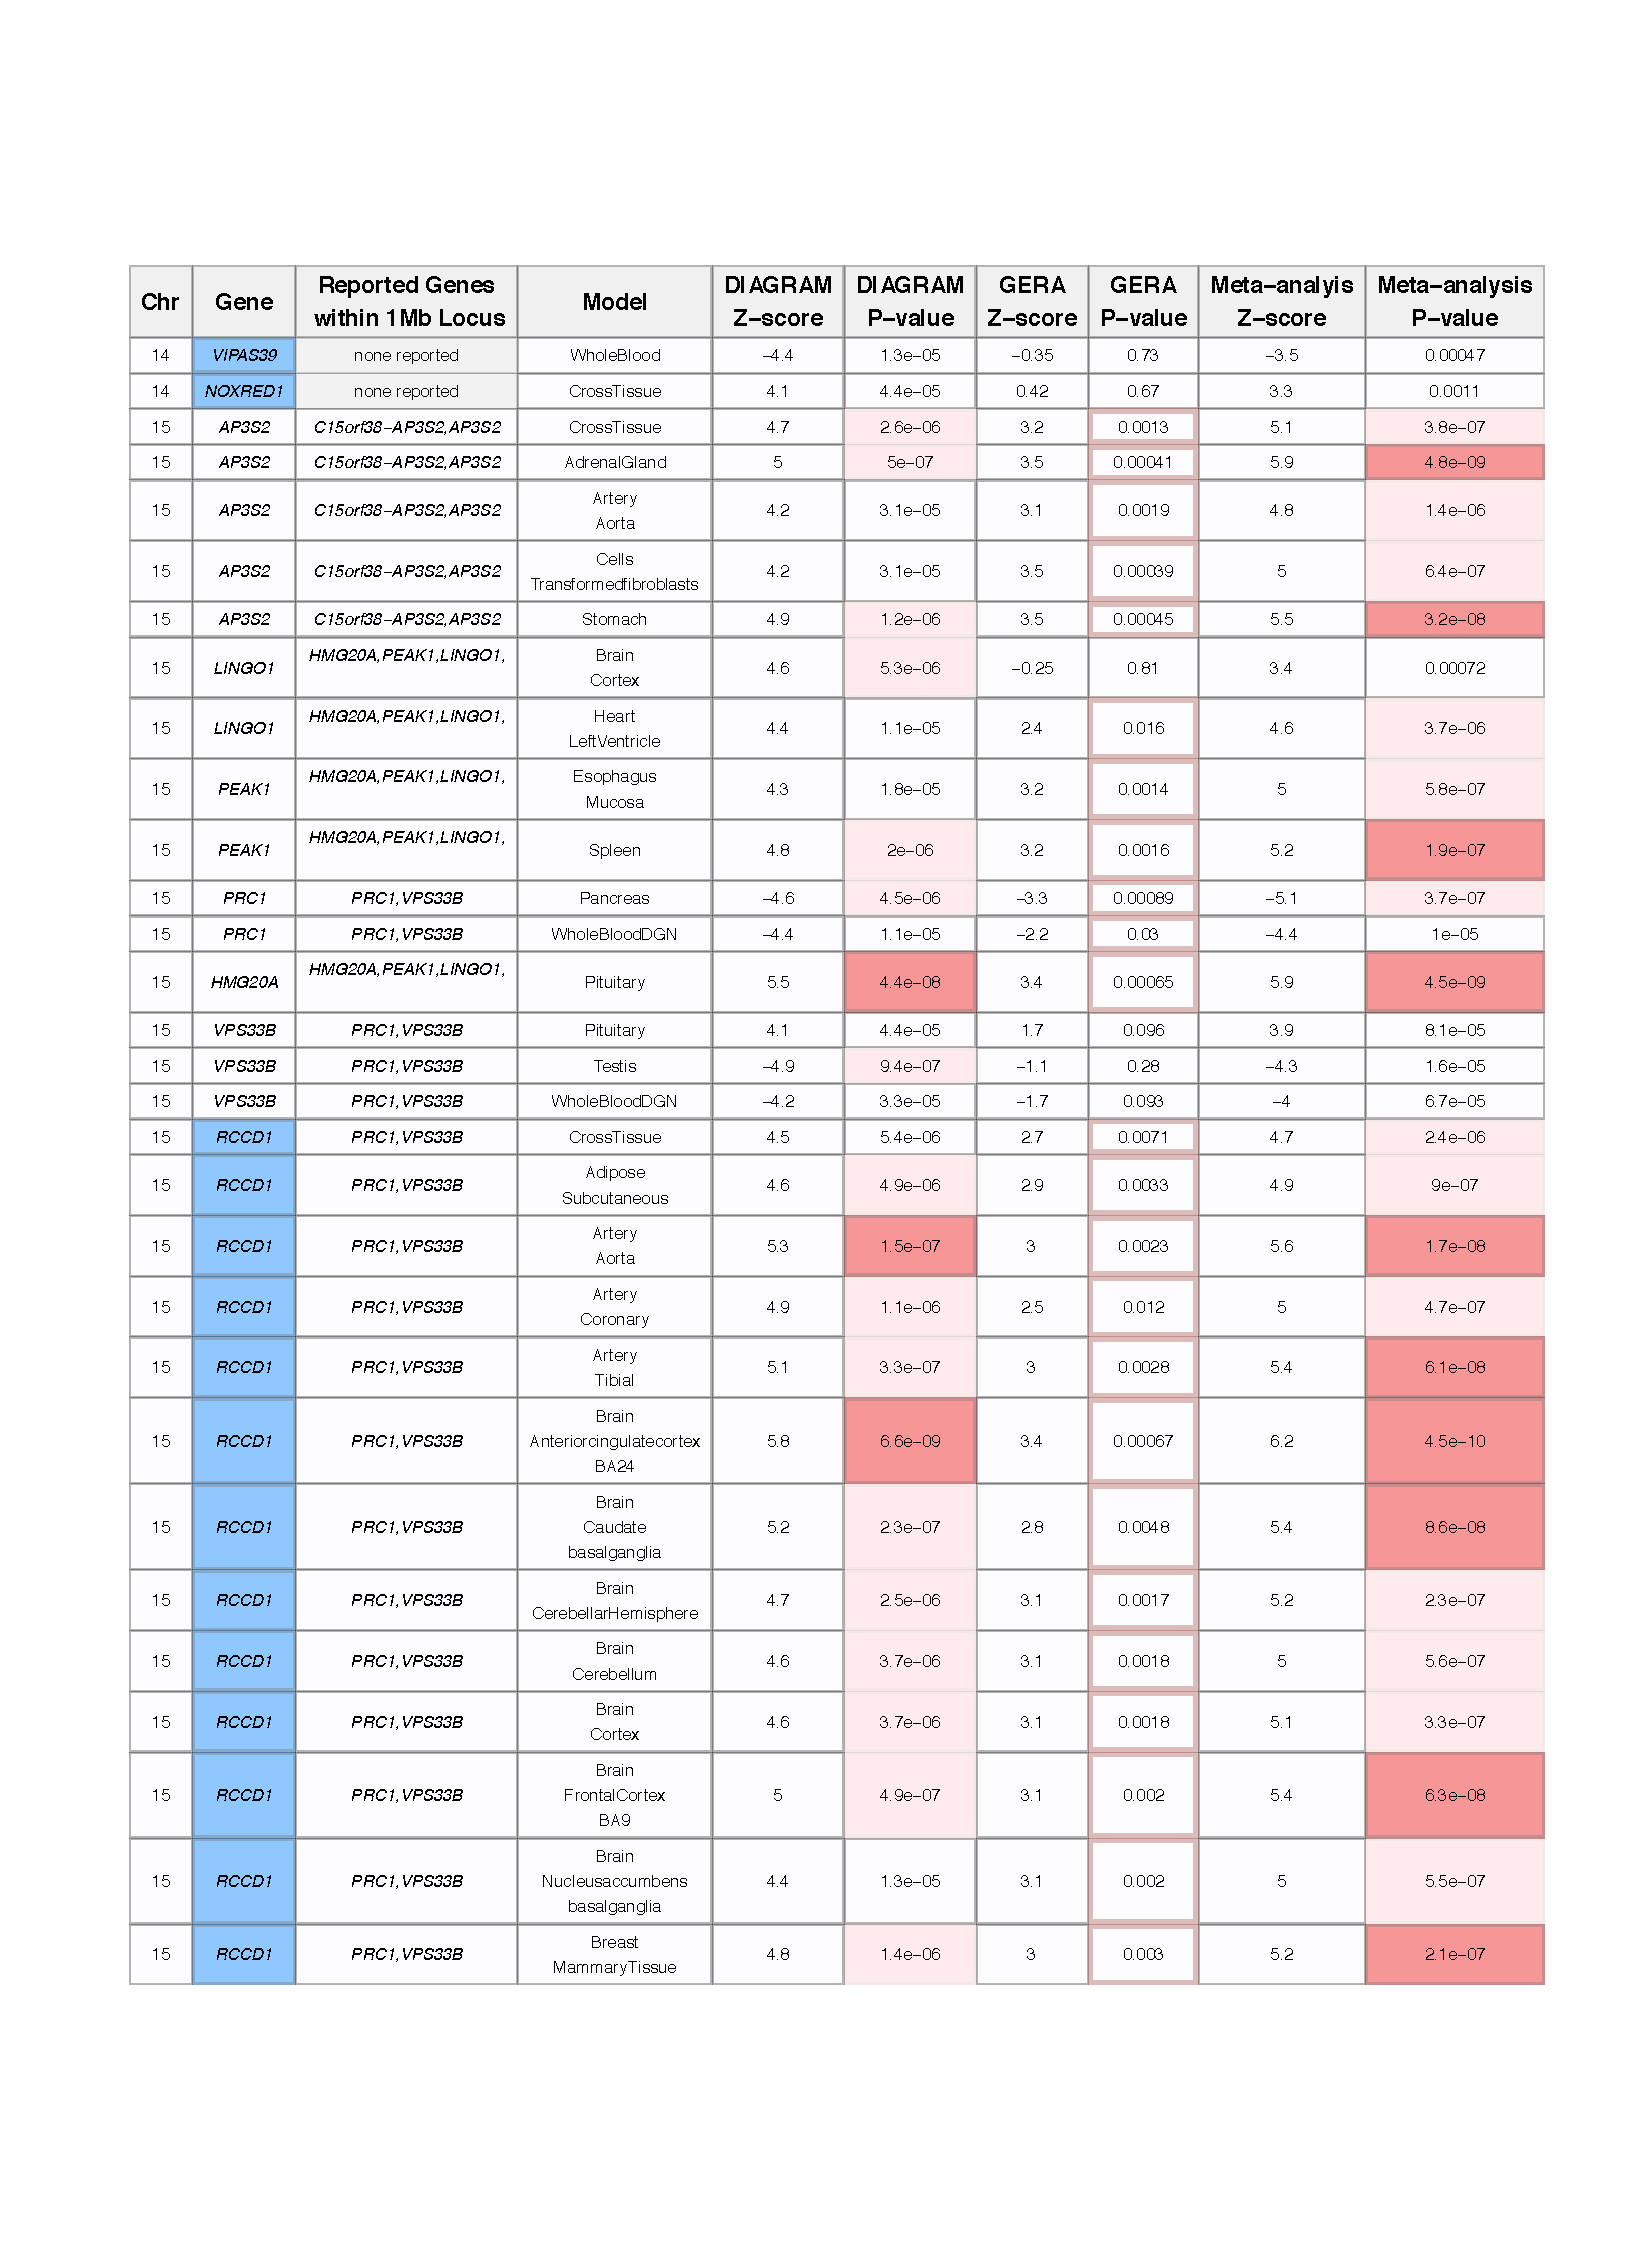
\includegraphics[width=0.90\textwidth]{supp_tab1_part5.pdf}
	\caption{\textbf{MetaXcan associations with T2D.} Results for genes and corresponding models that meet genome-wide significance \textit{in at least one model} from the DIAGRAM analysis are shown with nearby genes and results from the GERA replication study and meta-analysis of DIAGRAM and GERA Metaxcan associations. Blue shading denotes genes not implicated by the top $1,000$ SNPs from the DIAGRAM trans-ethnic meta-analysis of GWASs. Pink and red shading denote genome-wide significance in one model and across all models, respectively, for the DIAGRAM and meta-analysis. Replication in the GERA study is denoted by a pink outline.} 
	\label{tab:supp.table1.part5}
\end{table}

\clearpage
\begin{table}
\ContinuedFloat
	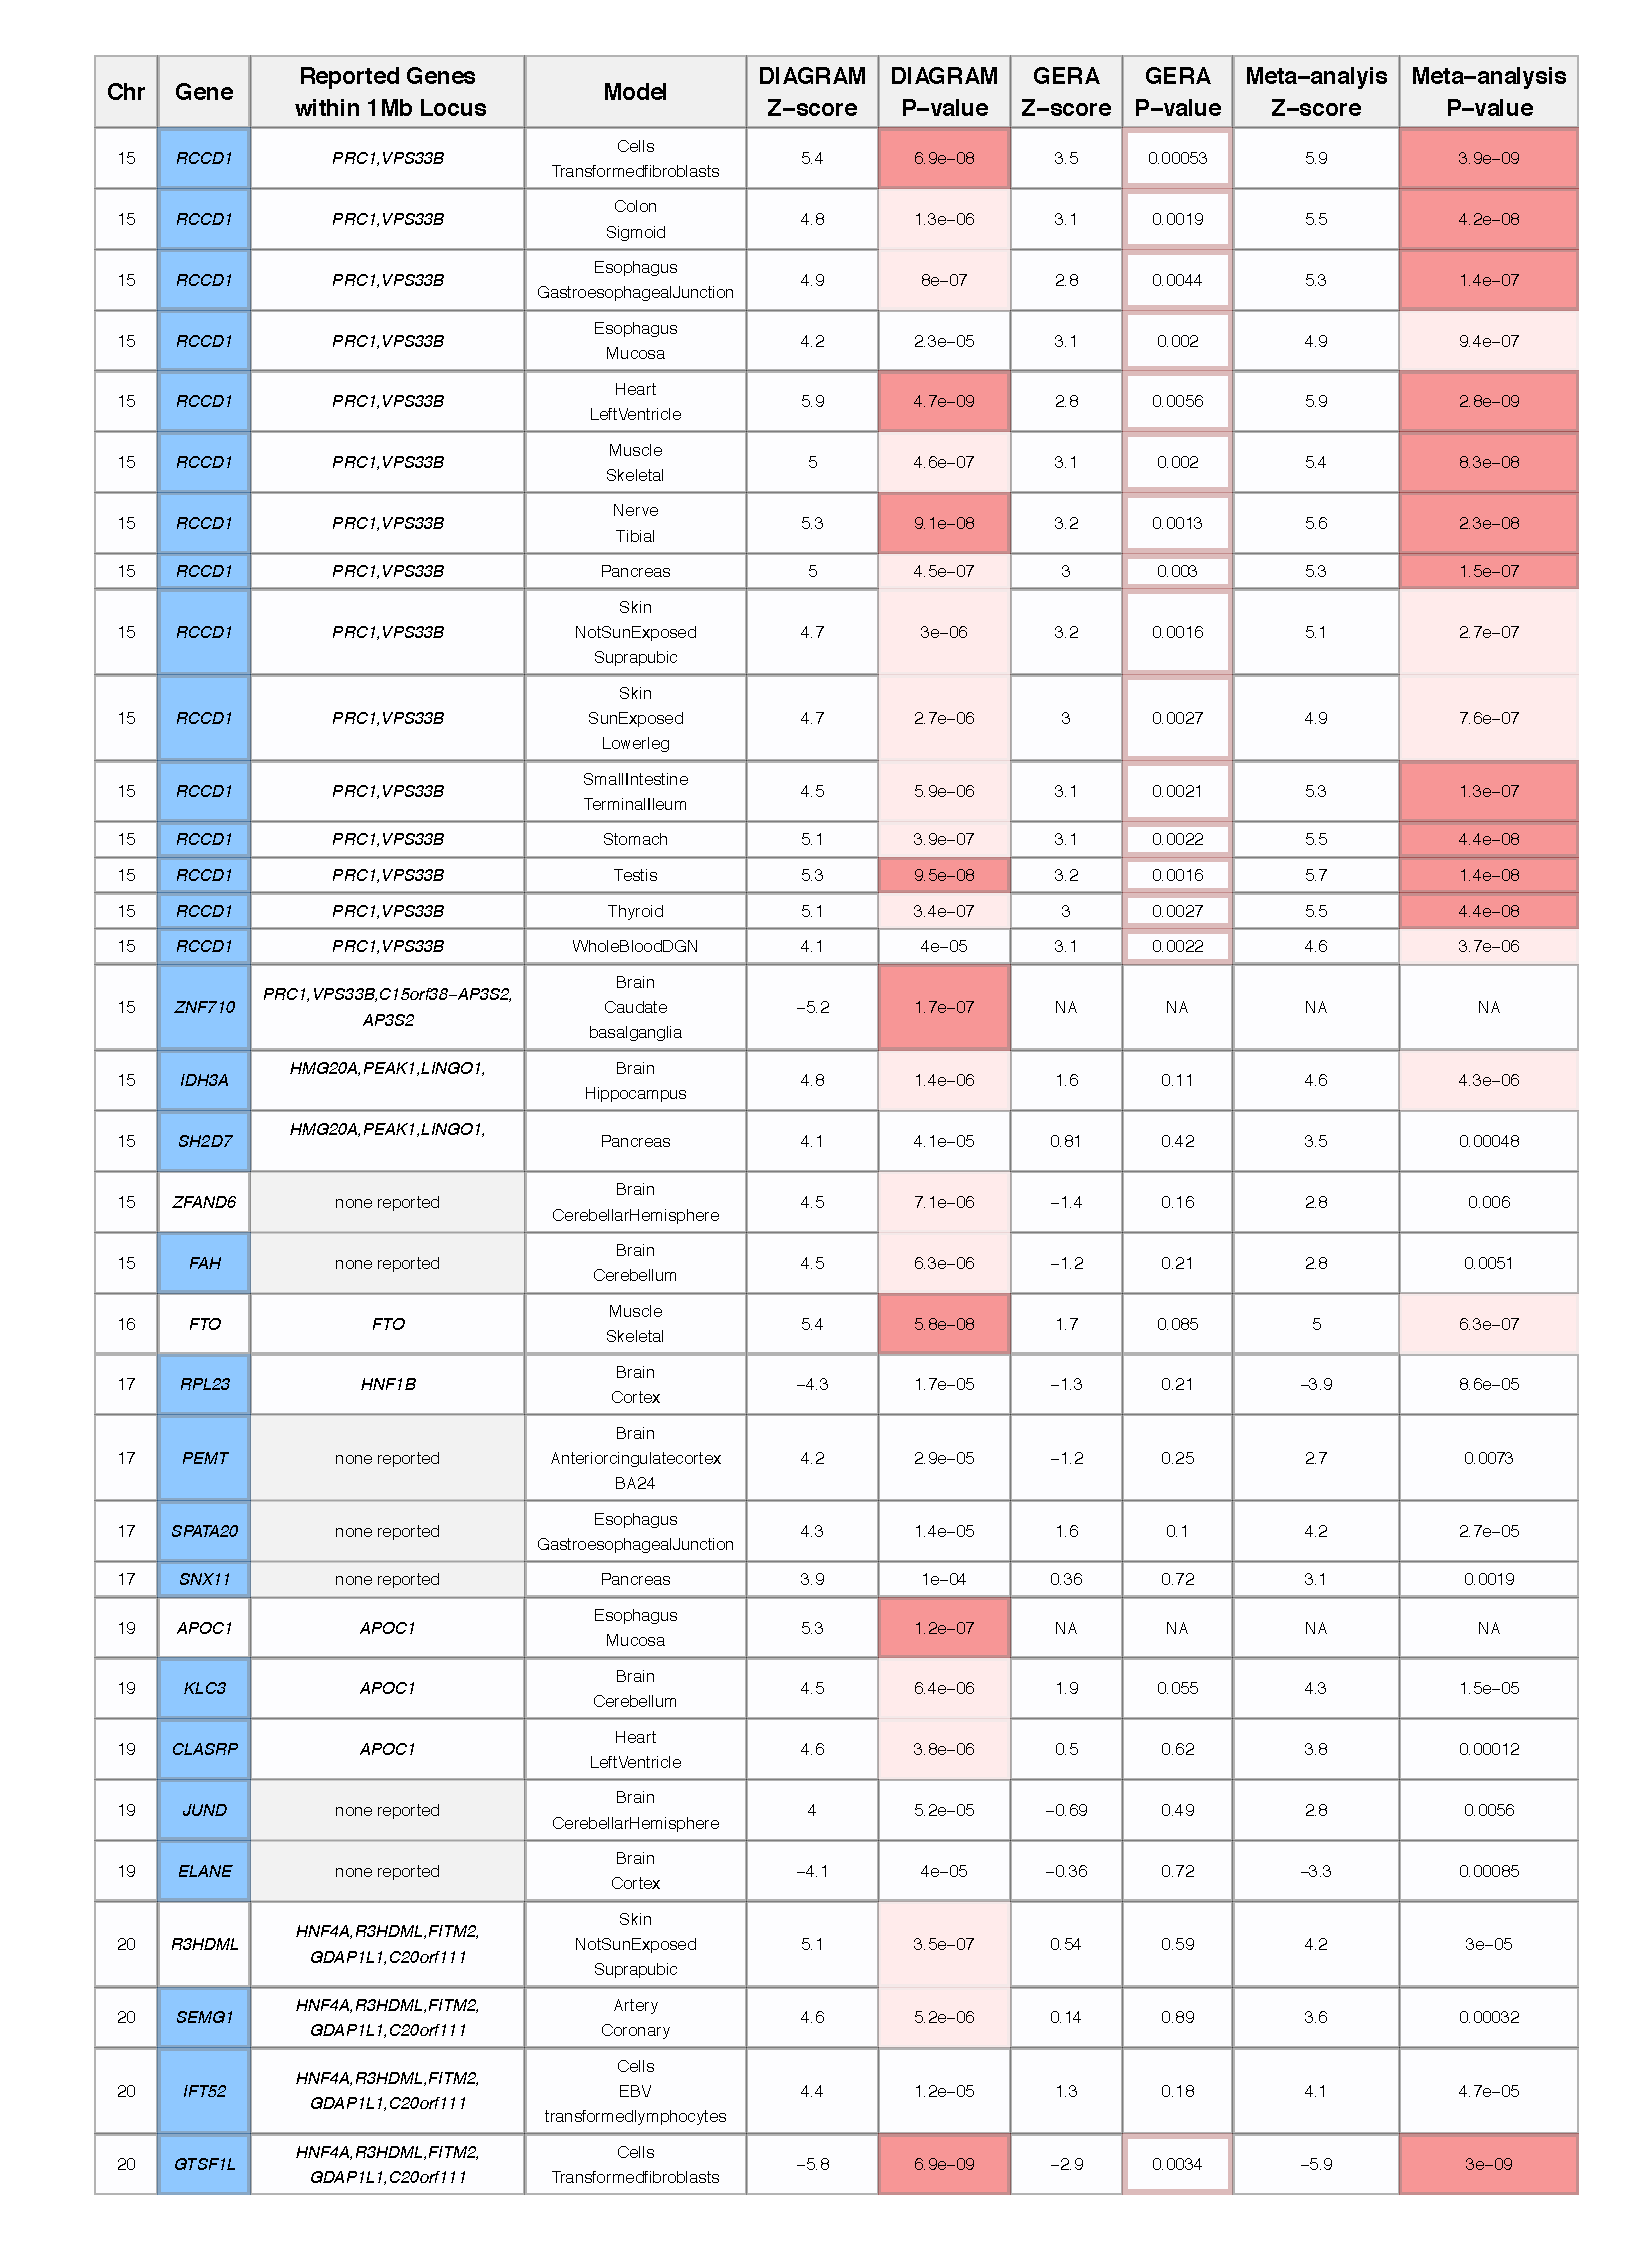
\includegraphics[width=0.76\textwidth]{supp_tab1_part6.pdf}
	\caption{\textbf{MetaXcan associations with T2D.} Results for genes and corresponding models that meet genome-wide significance \textit{in at least one model} from the DIAGRAM analysis are shown with nearby genes and results from the GERA replication study and meta-analysis of DIAGRAM and GERA Metaxcan associations. Blue shading denotes genes not implicated by the top $1,000$ SNPs from the DIAGRAM trans-ethnic meta-analysis of GWASs. Pink and red shading denote genome-wide significance in one model and across all models, respectively, for the DIAGRAM and meta-analysis. Replication in the GERA study is denoted by a pink outline.} 
	\label{tab:supp.table1.part6}
\end{table}

% Supplementary Table 2 

\begin{table}[!htbp] \centering 
\label{tab:supp.table2} 
\scalebox{0.85}{
\begin{tabular}{@{\extracolsep{5pt}} ccc} 
\\[-1.8ex]\hline 
\hline \\[-1.8ex] 
Rank & GO:BP Pathway & P-value \\ 
\hline \\[-1.8ex] 
$1$ & negative regulation of type B pancreatic cell apoptotic process & $0.0001$ \\ 
$2$ & AP-3 adaptor complex & $0.0002$ \\ 
$3$ & carbohydrate homeostasis & $0.0003$ \\ 
$4$ & glucose homeostasis & $0.0003$ \\ 
$5$ & regulation of type B pancreatic cell apoptotic process & $0.0004$ \\ 
$6$ & fat cell proliferation & $0.0004$ \\ 
$7$ & regulation of fat cell proliferation & $0.0004$ \\ 
$8$ & type B pancreatic cell apoptotic process & $0.0004$ \\ 
$9$ & monocarboxylic acid binding & $0.001$ \\ 
$10$ & core promoter binding & $0.001$ \\ 
$11$ & axolemma & $0.001$ \\ 
$12$ & multicellular organism growth & $0.001$ \\ 
$13$ & thyroid gland development & $0.001$ \\ 
$14$ & response to glucose & $0.002$ \\ 
$15$ & regulation of receptor biosynthetic process & $0.002$ \\ 
$16$ & response to hexose & $0.002$ \\ 
$17$ & negative regulation of cellular process & $0.002$ \\ 
$18$ & response to monosaccharide & $0.002$ \\ 
$19$ & receptor biosynthetic process & $0.002$ \\ 
$20$ & core promoter sequence-specific DNA binding & $0.002$ \\ 
$21$ & regulation of insulin secretion & $0.002$ \\ 
$22$ & response to carbohydrate & $0.003$ \\ 
$23$ & regulation of circadian rhythm & $0.003$ \\ 
$24$ & pancreas development & $0.003$ \\ 
$25$ & response to methyl methanesulfonate & $0.003$ \\ 
$26$ & cellular response to methyl methanesulfonate & $0.003$ \\ 
$27$ & regulation of N-terminal peptidyl-lysine acetylation & $0.003$ \\ 
$28$ & positive regulation of N-terminal peptidyl-lysine acetylation & $0.003$ \\ 
$29$ & negative regulation of ATF6-mediated unfolded protein response & $0.003$ \\ 
$30$ & response to metformin & $0.003$ \\ 
$31$ & negative regulation of pancreatic stellate cell proliferation & $0.003$ \\ 
$32$ & fumarylacetoacetase activity & $0.003$ \\ 
$33$ & hepatic duct development & $0.003$ \\ 
$34$ & hepatoblast differentiation & $0.003$ \\ 
$35$ & oxidative DNA demethylase activity & $0.003$ \\ 
$36$ & negative regulation of phosphatidylcholine catabolic process & $0.003$ \\ 
$37$ & respiratory system process & $0.003$ \\ 
$38$ & regulation of oligodendrocyte differentiation & $0.003$ \\ 
$39$ & fatty acid binding & $0.003$ \\ 
$40$ & epithelial tube branching involved in lung morphogenesis & $0.004$ \\ 
$41$ & regulation of collagen biosynthetic process & $0.004$ \\ 
$42$ & regulation of protein export from nucleus & $0.004$ \\ 
$43$ & regulation of cell proliferation & $0.004$ \\ 
$44$ & regulation of peptide hormone secretion & $0.004$ \\ 
$45$ & negative regulation of epithelial cell apoptotic process & $0.004$ \\ 
$46$ & response to testosterone & $0.004$ \\ 
$47$ & regulation of peptide secretion & $0.004$ \\ 
$48$ & insulin secretion & $0.004$ \\ 
$49$ & regulation of collagen metabolic process & $0.005$ \\ 
$50$ & regulation of multicellular organismal metabolic process & $0.005$ \\ 
\hline \\[-1.8ex] 
\end{tabular} 
}
\caption{\textbf{Biological pathways enriched among genes associated with T2D from MetaXcan analysis of DIAGRAM dataset.} The top 50 Gene Ontology Biological Process (GO:BP) pathways enriched among the set of MetaXcan-significant genes are shown with overrepresented p-value.} 
\end{table} 

% Supplementary Table 3 

\begin{table}[!htbp] \centering 
  \label{tab:supp.table3} 
\scalebox{0.85}{
\begin{tabular}{@{\extracolsep{5pt}} ccc} 
\\[-1.8ex]\hline 
\hline \\[-1.8ex] 
Rank & GO:BP Pathway & P-value \\ 
\hline \\[-1.8ex] 
$1$ & regulation of protein export from nucleus & $0.0001$ \\ 
$2$ & negative regulation of type B pancreatic cell apoptotic process & $0.0001$ \\ 
$3$ & carbohydrate homeostasis & $0.0001$ \\ 
$4$ & glucose homeostasis & $0.0001$ \\ 
$5$ & regulation of cell proliferation & $0.0002$ \\ 
$6$ & regulation of type B pancreatic cell apoptotic process & $0.0002$ \\ 
$7$ & fat cell proliferation & $0.0002$ \\ 
$8$ & regulation of fat cell proliferation & $0.0002$ \\ 
$9$ & type B pancreatic cell apoptotic process & $0.0003$ \\ 
$10$ & protein export from nucleus & $0.0004$ \\ 
$11$ & cyclin-dependent protein serine/threonine kinase inhibitor activity & $0.0005$ \\ 
$12$ & nuclear export & $0.0005$ \\ 
$13$ & multicellular organism growth & $0.001$ \\ 
$14$ & response to glucose & $0.001$ \\ 
$15$ & glial cell differentiation & $0.001$ \\ 
$16$ & oligodendrocyte differentiation & $0.001$ \\ 
$17$ & response to hexose & $0.001$ \\ 
$18$ & small molecule binding & $0.001$ \\ 
$19$ & thyroid gland development & $0.001$ \\ 
$20$ & response to monosaccharide & $0.001$ \\ 
$21$ & regulation of receptor biosynthetic process & $0.001$ \\ 
$22$ & regulation of cyclin-dependent protein serine/threonine kinase activity & $0.002$ \\ 
$23$ & response to carbohydrate & $0.002$ \\ 
$24$ & receptor biosynthetic process & $0.002$ \\ 
$25$ & pancreas development & $0.002$ \\ 
$26$ & heterocyclic compound binding & $0.002$ \\ 
$27$ & cell proliferation & $0.002$ \\ 
$28$ & regulation of sequence-specific DNA binding transcription factor activity & $0.002$ \\ 
$29$ & gliogenesis & $0.002$ \\ 
$30$ & negative regulation of transcription from RNA polymerase II promoter & $0.002$ \\ 
$31$ & growth & $0.002$ \\ 
$32$ & cyclin-dependent protein serine/threonine kinase regulator activity & $0.002$ \\ 
$33$ & organic cyclic compound binding & $0.002$ \\ 
$34$ & regulation of oligodendrocyte differentiation & $0.002$ \\ 
$35$ & respiratory system process & $0.002$ \\ 
$36$ & transcription from RNA polymerase II promoter & $0.002$ \\ 
$37$ & epithelial tube branching involved in lung morphogenesis & $0.003$ \\ 
$38$ & protein serine/threonine kinase inhibitor activity & $0.003$ \\ 
$39$ & viral capsid & $0.003$ \\ 
$40$ & regulation of N-terminal peptidyl-lysine acetylation & $0.003$ \\ 
$41$ & positive regulation of N-terminal peptidyl-lysine acetylation & $0.003$ \\ 
$42$ & negative regulation of ATF6-mediated unfolded protein response & $0.003$ \\ 
$43$ & oxidative DNA demethylase activity & $0.003$ \\ 
$44$ & hepatic duct development & $0.003$ \\ 
$45$ & hepatoblast differentiation & $0.003$ \\ 
$46$ & response to metformin & $0.003$ \\ 
$47$ & negative regulation of pancreatic stellate cell proliferation & $0.003$ \\ 
$48$ & protein stabilization & $0.003$ \\ 
$49$ & nucleotide binding & $0.003$ \\ 
$50$ & nucleoside phosphate binding & $0.003$ \\ 
\hline \\[-1.8ex] 
\end{tabular} 
}
\caption{\textbf{Biological pathways enriched among genes associated with T2D from meta-analysis of results from MetaXcan analyses of DIAGRAM and GERA datasets.} The top 50 Gene Ontology Biological Process (GO:BP) pathways enriched among the set of MetaXcan-significant genes are shown with overrepresented p-value.}  
\end{table} 

%Supplementary Table 4 
\begin{table}[!htbp] \centering 
  \label{tab:supp.table4} 
\scalebox{0.80}{
\begin{tabular}{@{\extracolsep{5pt}} ccc} 
\\[-1.8ex]\hline 
\hline \\[-1.8ex] 
Rank & GO:BP Pathway & P-value \\ 
\hline \\[-1.8ex] 
$1$ & fumarylacetoacetase activity & $0.0003$ \\ 
$2$ & hydrolase activity, acting on acid carbon-carbon bonds & $0.001$ \\ 
$3$ & hydrolase activity, acting on acid carbon-carbon bonds, in ketonic substances & $0.001$ \\ 
$4$ & positive regulation of circadian sleep/wake cycle, REM sleep & $0.001$ \\ 
$5$ & negative regulation of glomerular filtration & $0.001$ \\ 
$6$ & negative regulation of urine volume & $0.001$ \\ 
$7$ & negative regulation of renal sodium excretion & $0.001$ \\ 
$8$ & tyrosine catabolic process & $0.001$ \\ 
$9$ & regulation of circadian sleep/wake cycle, wakefulness & $0.001$ \\ 
$10$ & positive regulation of circadian sleep/wake cycle, wakefulness & $0.001$ \\ 
$11$ & circadian sleep/wake cycle, wakefulness & $0.001$ \\ 
$12$ & regulation of circadian sleep/wake cycle, REM sleep & $0.001$ \\ 
$13$ & positive regulation of circadian sleep/wake cycle, sleep & $0.002$ \\ 
$14$ & positive regulation of synaptic transmission, cholinergic & $0.002$ \\ 
$15$ & circadian sleep/wake cycle, REM sleep & $0.002$ \\ 
$16$ & arginine catabolic process & $0.002$ \\ 
$17$ & negative regulation of heart rate & $0.002$ \\ 
$18$ & tyrosine metabolic process & $0.002$ \\ 
$19$ & L-phenylalanine catabolic process & $0.003$ \\ 
$20$ & erythrose 4-phosphate/phosphoenolpyruvate family amino acid catabolic process & $0.003$ \\ 
$21$ & regulation of synaptic transmission, cholinergic & $0.003$ \\ 
$22$ & positive regulation of fibroblast migration & $0.003$ \\ 
$23$ & regulation of glomerular filtration & $0.003$ \\ 
$24$ & L-phenylalanine metabolic process & $0.003$ \\ 
$25$ & erythrose 4-phosphate/phosphoenolpyruvate family amino acid metabolic process & $0.003$ \\ 
$26$ & glomerular filtration & $0.004$ \\ 
$27$ & protein targeting to peroxisome & $0.004$ \\ 
$28$ & peroxisomal transport & $0.004$ \\ 
$29$ & protein localization to peroxisome & $0.004$ \\ 
$30$ & establishment of protein localization to peroxisome & $0.004$ \\ 
$31$ & positive regulation of circadian rhythm & $0.004$ \\ 
$32$ & renal system process involved in regulation of blood volume & $0.004$ \\ 
$33$ & renal filtration & $0.004$ \\ 
$34$ & arginine metabolic process & $0.004$ \\ 
$35$ & regulation of circadian sleep/wake cycle, sleep & $0.004$ \\ 
$36$ & regulation of urine volume & $0.005$ \\ 
$37$ & negative regulation of heart contraction & $0.005$ \\ 
$38$ & renal sodium excretion & $0.005$ \\ 
$39$ & regulation of renal sodium excretion & $0.005$ \\ 
$40$ & regulation of circadian sleep/wake cycle & $0.005$ \\ 
$41$ & positive regulation of collagen metabolic process & $0.005$ \\ 
$42$ & positive regulation of collagen biosynthetic process & $0.005$ \\ 
$43$ & positive regulation of multicellular organismal metabolic process & $0.005$ \\ 
$44$ & aromatic amino acid family catabolic process & $0.005$ \\ 
$45$ & circadian sleep/wake cycle, sleep & $0.005$ \\ 
$46$ & positive regulation of heart rate & $0.005$ \\ 
$47$ & positive regulation of vasodilation & $0.006$ \\ 
$48$ & renal system process involved in regulation of systemic arterial blood pressure & $0.006$ \\ 
$49$ & circadian sleep/wake cycle process & $0.006$ \\ 
$50$ & glutamine family amino acid catabolic process & $0.006$ \\ 
\hline \\[-1.8ex] 
\end{tabular} 
}
\caption{\textbf{Biological pathways enriched among ``unknown'' loci genes associated with T2D from MetaXcan analysis of DIAGRAM dataset.} The top 50 Gene Ontology Biological Process (GO:BP) pathways enriched among the set of MetaXcan-significant genes located beyond 1 Mb of the top 89 putative T2D genes reported from the DIAGRAM meta-analysis of GWASs are shown with overrepresented p-value.} 
\end{table} 


\begin{table}[!htbp] \centering 
  \label{} 
\scalebox{0.68}{
\begin{tabular}{@{\extracolsep{5pt}} cccc} 
\\[-1.8ex]\hline 
\hline \\[-1.8ex] 
Trait & P-value & Reported T2D Genes & Novel Genes \\ 
\hline \\[-1.8ex] 
Type 2 diabetes & $0.00001$ & \textit{TCF7L2, HHEX, FTO} &  \\ 
 &  & \textit{JAZF1, HMG20A, WFS1} &  \\
 &  & \textit{PPARG, TP53INP1, R3HDML} &  \\ 
 &  & \textit{PRC1, AP3S2, INTS8} &  \\ 
 &  & \textit{MPHOSPH9, KLHDC5, CAMK1D} &  \\ 
 &  & \textit{KCNJ11, ANK1, AP3S2, ZFAND6} &  \\ 
Type 2 diabetes and other traits & $0.0002$ & \textit{TCF7L2, WFS1} &  \\ 
Body mass index & $0.0004$ & \textit{TCF7L2, FTO, KCNJ11} & \textit{DGKG} \\ 
 &  & \textit{PPARG, CPNE4} &  \\ 
HIV-1 control & $0.001$ &  & \textit{ZNRD1, HLA-A} \\ 
IgE levels & $0.001$ &  & \textit{HCG27, HLA-A} \\ 
Fasting insulin-related traits (interaction with BMI) & $0.002$ & \textit{TCF7L2, PPARG} &  \\ 
Weight & $0.002$ & \textit{FTO}  & \textit{DGKG} \\ 
Glycated hemoglobin levels & $0.002$ & \textit{TCF7L2, ANK1} &  \\ 
Sasang constitutional medicine type (So-Eum) & $0.003$ & \textit{FTO} &  \\ 
Body mass in chronic obstructive pulmonary disease & $0.003$ & \textit{FTO} &  \\ 
Drug-induced liver injury (amoxicillin-clavulanate) & $0.003$ & \textit{HLA-A} &  \\ 
Drug-induced liver injury & $0.003$ & \textit{PPARG} &  \\ 
Breast cancer & $0.005$ & \textit{TCF7L2, FTO, PRC1} &  \\ 
Free thyroxine concentration & $0.006$ & \textit{JAZF1} &  \\ 
Height adjusted BMI & $0.006$ & \textit{FTO} & \\ 
Essential tremor & $0.006$ & \textit{LINGO1} &  \\ 
Metabolic syndrome & $0.006$ & \textit{TCF7L2, FTO} &  \\ 
Breast Cancer in BRCA1 mutation carriers & $0.007$ & \textit{TCF7L2} &  \\ 
Change in intraocular pressure in response to  & $0.009$ &  & \textit{HLA-A} \\ 
steroid treatment (triamcinolone acetonide) &  &  &  \\ 
Apolipoprotein Levels & $0.009$ & \textit{APOC1} &  \\ 
Vitiligo & $0.012$ &  & \textit{CASP7, HLA-A} \\ 
Biomedical quantitative traits & $0.012$ & \textit{FTO} &  \\ 
Vincristine-induced peripheral neuropathy  & $0.015$ & \textit{NDUFAF6} &  \\ 
in acute lymphoblastic leukemia &  &  &  \\
Educational attainment & $0.015$ & \textit{MPHOSPH9} & \textit{C12orf65} \\ 
Two-hour glucose challenge & $0.016$ & \textit{TCF7L2} &  \\ 
Beta-2 microglubulin plasma levels & $0.021$ &  & \textit{HLA-A} \\ 
Triglycerides & $0.021$ & \textit{FTO, APOC1} &  \\ 
Dietary macronutrient intake & $0.021$ & \textit{FTO} &  \\ 
Complement C3 and C4 levels & $0.022$ &  & \textit{HLA-A}  \\ 
Adiposity & $0.023$ & \textit{FTO} &  \\ 
Nasopharyngeal carcinoma & $0.025$ &  & \textit{HLA-A} \\ 
Bone mineral density & $0.026$ & \textit{KLHDC5} & \textit{SOX4} \\ 
Osteoarthritis & $0.026$ & \textit{FTO} &  \\ 
Bone mineral density (paediatric, lower limb) & $0.027$ & \textit{KLHDC5} &  \\ 
Bipolar disorder (body mass index interaction) & $0.027$ & \textit{TCF7L2} &  \\ 
Plasminogen activator inhibitor type 1 levels (PAI-1) & $0.028$ & \textit{PPARG} &  \\ 
Dehydroepiandrosterone sulphate levels & $0.028$ & \textit{HHEX} &  \\ 
LDL cholesterol & $0.030$ & \textit{APOC1}  & \textit{GPAM} \\ 
Retinopathy in non-diabetics & $0.031$ & \textit{KLHDC5} &  \\ 
Cholesterol, total & $0.034$ & \textit{APOC1} & \textit{GPAM} \\ 
QT interval (interaction) & $0.034$ & \textit{CAMK1D}   & \\ 
Proinsulin levels & $0.034$ & \textit{TCF7L2} &  \\ 
Bone mineral density (paediatric, total body less head) & $0.039$ & \textit{KLHDC5} &  \\ 
Obesity (extreme) & $0.040$ & \textit{FTO} &  \\ 
Pulmonary function decline & $0.042$ & \textit{ANK1} &  \\ 
AIDS progression & $0.042$ &  & \textit{ZNRD1} \\ 
Alzheimer's disease (age of onset) & $0.046$ & \textit{APOC1} &  \\ 
Fasting glucose-related traits & $0.050$ & \textit{TCF7L2} &  \\ 
\hline \\[-1.8ex] 
\end{tabular}
}
	\caption{\textbf{MetaXcan-significant genes overlap with putative trait genes implicated by GWAS across multiple complex traits.} We performed a sampling study to to test for enrichment of putative trait genes among the set of T2D genes implicated by our MetaXcan analysis of the DIAGRAM trans-ethnic study. The enrichment p-value is shown for each trait that significantly shares putative genes (implicated by GWAS) in common with the set of MetaXcan-signficant T2D genes. Moreover, the table shows the shared genes for each trait and indicates whether the gene is a putative T2D gene (i.e. either in the set of $89$ genes implicated by the top $1,000$ SNPs from the DIAGRAM trans-ethnic study or reported in the NHGRI-EBI catalogue for “Type 2 diabetes”) or is a novel candidate T2D gene implicated by MetaXcan. } 
\end{table}  





\end{document} 